%! TEX root = ms.tex
%! TEX program = pdflatex
\documentclass{elsarticle}
\usepackage{geometry}
\geometry{left=3cm, right=3cm, top=2.5cm, bottom=2.5cm} 
\usepackage{lineno,hyperref}
\usepackage{amsmath, amsthm}
\usepackage{relsize}
\usepackage{booktabs}
\usepackage{makecell}
\usepackage{lscape}
\usepackage{xcolor}
\usepackage{subfig}
\modulolinenumbers[5]
\bibliographystyle{elsarticle-num}


\begin{document}

\begin{frontmatter}

	\title{Analyzing Performance Bottleneck in Graph Neural Network Training: An Experimental View}
	\author{Zhaokang Wang, Yunpan Wang, Chunfeng Yuan, Yihua Huang\corref{correspondingauthor}}
	\cortext[correspondingauthor]{Corresponding author}
	\ead{\{wangzhaokang, wangyp\}@smail.nju.edu.cn, \{cfyuan, yhuang\}@nju.edu.cn}
	\address{State Key Laboratory for Novel Software Technology, Department of Computer Science and Technology, Nanjing University, Nanjing 210023, China}

	\begin{abstract}
		Graph neural network has become a research hotspot in the field of artificial intelligence due to state-of-the-art of performance
		achieved in many grpah-related tasks. At the same time, various of graph neural network system has emrged one after another.
		These systems have used their own skills in implementation, but there are very few works to study the performance bottleneck
		on graph neural network training. In contrast to prior works that present characterization of GCNs and select GNNs cover GNN workloads,
		we select typical algorithms by complexity of edge/vertex calculation. We analyze the performance bottleneck by breaking down training
		time, study the affects of hyper-parameters and sampling technologies and find factors of memory usage. We finally put forward some key
		findings for GNN training and hope our work can help GNN system researchers.
	\end{abstract}

	\begin{keyword}
		graph neural network, performance bottleneck, deep learning, characterization
	\end{keyword}

\end{frontmatter}

\linenumbers

\section{Introduction}

In recent years, the graph neural network (GNN) becomes a hot research topic in the field of artificial intelligence.
%
Many GNNs~\cite{kipf2017_gcn, defferrad2016_chebnet, li2018_agcn,li2015_ggnn, hamilton2017_graphsage, huang2018_gat, zhang2018_gaan} are proposed.
%
They can learn the representation of vertices/edges in a graph from its topology and the original feature vectors in an \emph{end-to-end} manner.
%
The powerful expression capability makes GNNs achieve good accuracy in not only graph analytical tasks \cite{zhou2018_gnn_review, zhang2018_gnn_survey, comprehensive-survey-wu-2020} (like node classification and link prediction) but also computer vision tasks (like human-object interaction \cite{qi2018_learning_humanobject}, human parsing \cite{wang2020_hierarchical_human_parsing}, and video object segmentation \cite{wang2019_zeroshot_video}).

To train GNNs easily, a series of GNN libraries/systems \cite{PyG, DGL, ma2019_neugraph, zhu2019_aligraph, PGL} are proposed.
%
PyTorch Geometric (PyG) \cite{PyG}, NeuGraph \cite{ma2019_neugraph}, PGL \cite{PGL} and Deep Graph Library (DGL) \cite{DGL} build upon the existing deep learning frameworks (PyG on PyTorch, NeuGraph on TensorFlow, PGL on PaddlePaddle, DGL on multiple backends).
%
They provide users with a high-level programming model (the message-passing framework for PyG/PGL/DGL and the SAGA-NN model for NeuGraph) to describe the structure of a GNN.
%
They take advantage of the common tools provided by the underlying frameworks like the automatic differentiation to simplify the development.
%
They utilize specially optimized CUDA kernels (like kernel fusion \cite{DGL, ma2019_neugraph}) and other implementation techniques (like 2D graph partitioning \cite{ma2019_neugraph}) to improve the speed of GNN training on GPUs.

However, what is the real performance bottleneck in GNN training and inference is still in doubt.
%
Yan et al. \cite{yan2020_characterizing_gcn} and Zhang et al. \cite{zhang2020_analysis_neugraph} experimentally analyze the architectural characteristics of GNN \emph{inference}.
%
They find that the GNN inference is more cache-friendly than the traditional graph analysis tasks (like PageRank) and is suitable for GPUs.
%
They verify the effectiveness of the kernel fusion optimization in reducing the time of inference.
%
Nevertheless, they only analyze the inference stage, ignoring the effects of the backpropagation during training.

To explore essential performance bottlenecks in both GNN training and inference, we conduct a range of experimental analysis in this work.
%
We focus on the efficiency bottlenecks of GNN training and inference.
%
We model the GNNs with the message-passing framework that decomposes a GNN layer into two parts: the vertex calculation and the edge calculation.
%
According to the time complexity of the two parts, we classify the typical GNNs into four quadrants (\{high, low\} complexity $\times$ \{vertex, edge\} calculation).
%
We choose GCN \cite{kipf2017_gcn}, GGNN \cite{li2015_ggnn}, GAT \cite{huang2018_gat}, and GaAN \cite{zhang2018_gaan} as representative GNNs of the four quadrants.

We implement them with PyG and evaluate their efficiency and accuracy with six real-world datasets on a GPU card.
%
We identify the most time-consuming stage in GNN training and inference by decomposing the training and inference time per epoch from the layer level to the operator level.
%
We also analyze the memory usage during training and inference to discover the main factor that limits the data scalability of GNN training and inference on GPUs. 
%
Finally, we evaluate whether or not the sampling techniques affect the performance bottlenecks and accuracy.
%
The key findings and insights are summarized below.

\begin{itemize}
    \item \emph{The training and inference time and the memory usage of a GNN layer are mainly affected by the dimensions of the input/output hidden vectors.}
    %
    Fixing other hyper-parameters, the training and inference time and the memory usage of a GNN layer increase linearly with the dimensions.
    
    \item \emph{The edge-related calculation is the performance bottleneck for most GNNs.}
    For GNNs with high edge calculation complexity, most of the training and inference time is spent on conducting the messaging function for every edge.
    %
    For GNNs with low edge calculation complexity, the collection and aggregation of message vectors of all edges consume most of the training and inference time.
    
    \item \emph{The high memory usage of the edge calculation stage is the main factor limiting the data scalability of GNN training and inference.}
    %
    The edge calculation generates (and caches) many intermediate results.
    %
    They are an order of magnitude larger than the dataset itself.
    %
    As GPUs have limited on-chip memory, high memory consumption prevents us from performing training and inference on big graphs.
    
    \item \emph{The sampling techniques can significantly reduce the memory usage of training and inference.}
    %
    The sampling techniques are essential for performing GNN training and inference on big graphs with GPUs.
    %
    The accuracy of the GNN models trained with the sampling techniques is close to the accuracy of full-batch training.
    %
    However, the existing implementation of sampling is still inefficient.
    % 
    The time spent on sampling may exceed the time spent on training and inference.
    Under small batch sizes, the sampled graphs are also small, wasting the computing power of GPUs.
\end{itemize}

Based on the insights, we provide several potential optimization directions:

\begin{itemize}
      \item To reduce training and inference time, \emph{optimizations should focus on improving the efficiency of the edge calculation}.
      % 
      One may consider developing optimized operators for the messaging step that is the major source of computing costs in the edge calculation.
      %
       Fusing operators of the collection step, messaging function and the aggregation step together is another way to reduce the overheads in the edge calculation.
       
      \item To reduce memory usage, \emph{optimizations should focus on reducing the intermediate results in the edge calculation}.
      %
      One may consider adopting the checkpoint mechanism to cache less intermediate results during the forward phase and re-calculate the needed data on the fly during the backpropagation.
      %
      \item To improve the efficiency of the sampling techniques, \emph{one may consider overlapping the sampling on the CPU side with the training/inference on the GPU side.}
      %
      Choosing a proper batch size automatically is another potential optimization.
\end{itemize}

We hope that our analysis can help the developers of the GNN libraries/systems have a better understanding of the characteristics of GNN training/inference and propose more targeted optimizations.

\paragraph{Outline}
We briefly survey the typical GNNs in Section~\ref{sec:review_of_gnns}.
%
We introduce our experimental setting and targets in Section~\ref{sec:experimental_design}.
%
The experimental results are presented and analyzed in Section~\ref{sec:experiment_results}.
%
We summarize the key findings and give out potential optimization directions in Section~\ref{sec:insights}.
%
We introduce the related work in Section~\ref{sec:related_work} and conclude our work in Section~\ref{sec:conclusion}.

\section{Review of Graph Neural Networks}

In this section, we formally define the graph neural network (GNN, for short) and breifly survey typical graph neural networks.
We denote a simple graph $\mathcal{G}$ as $\mathcal{G}=(\mathcal{V}, \mathcal{E})$, where $\mathcal{V}$ and $\mathcal{E}$ are the vertex set and the edge set of $\mathcal{G}$, respectively.
Let $n=|\mathcal{V}|$ and $m=|\mathcal{E}|$ as the number of vertices/edges.
We use $v_i$ $(0 \leq i < n)$ to denote a vertex and $e_{i,j}=(v_i, v_j)$ to denote the edge pointing from $v_i$ to $v_j$.
The adjacency set of $v_i$ is $\mathcal{N}(v_i)=\{v|(v_i, v) \in \mathcal{E}\}$.
We denote a \emph{vector} with a bold lower case letter like $\boldsymbol{x}$ and a \emph{matri}x with a bold upper case letter like $\boldsymbol{X}$.

\subsection{General Structure of Graph Neural Networks}

As illustracted in \figurename~\ref{fig:general_structure_of_gnn}, a typical GNN can be decomposed into three parts: an input layer + several GNN layers + a prediction layer.

\begin{figure}
	\centering
	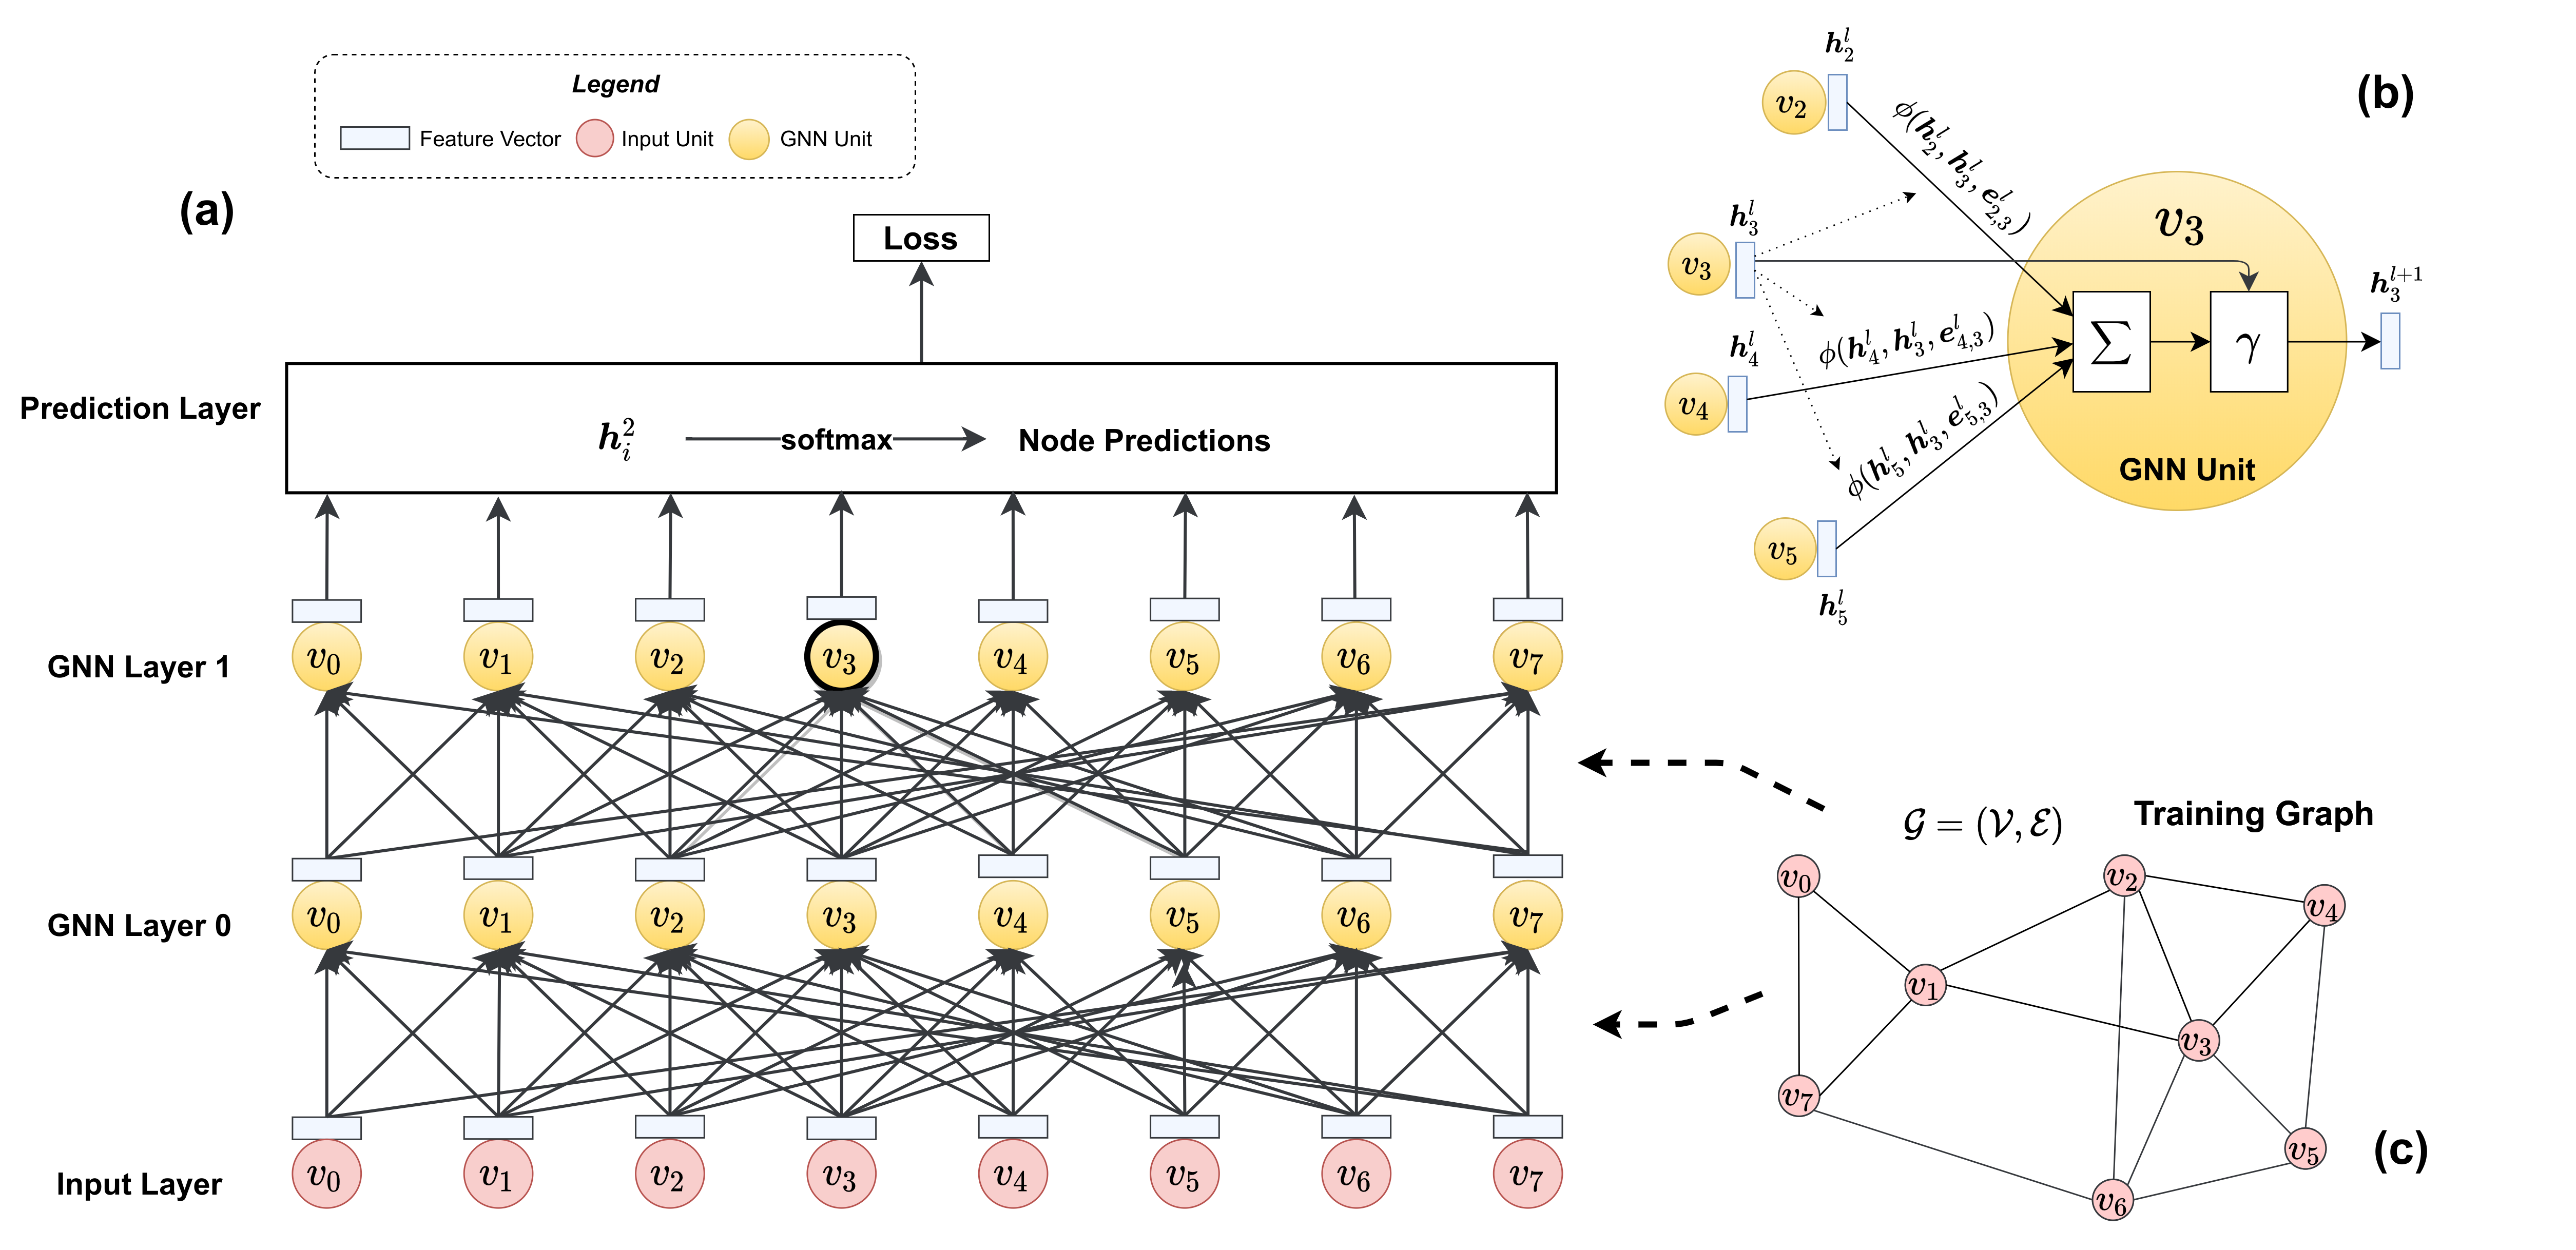
\includegraphics[width=1\columnwidth]{figs/illustration/GNN_common_architecture.png}
	\caption{Structure of a typical graph neural network. (a) Demo GNN, (b) Demo graph. The target application is the node classification. The demo GNN has two GNN layers.}
	\label{fig:general_structure_of_gnn}
\end{figure}

A GNN receives a graph $\mathcal{G}$ as the input.
Every vertex $v_i$ in $\mathcal{G}$ is attached with a feature vector $\boldsymbol{x}_i$ to describe the properties of the vertex.
The edges of $\mathcal{G}$ may also be attached with feature vectors $\boldsymbol{e}_{i,j}$
The input layer of a GNN receives feature vectors from all vertices and passes them to GNN layers.

A GNN layer consists of $n$ graph neurons, where $n$ is the number of vertices in $\mathcal{G}$.
Each graph neuron corresponds to a vertex in $\mathcal{G}$.
In the first GNN layer (Layer 0), the graph neuron of the vertex $v_i$ collects input feature vectors of itself and the vertices $\boldsymbol{x}_j$ that are adjacent to $v_i$ in $\mathcal{G}$ (i.e., $v_j \in \mathcal{N}(v_i)$) from the input layer.
After aggregating input feature vectors and applying non-linear transformation, the graph neuron outputs a hidden feature vector $\boldsymbol{h}^1_i$ for $v_i$.
Take the demo DNN in \figurename~\ref{fig:general_structure_of_gnn}(a) as the example.
Since $\mathcal{N}(v_3) = \{v_1, v_2, v_4, v_5, v_6\}$, the graph neuron of $v_1$ at layer 0 collects the feature vectors \{$\boldsymbol{x}_1$, $\boldsymbol{x}_2$, $\boldsymbol{x}_3$, $\boldsymbol{x}_4$, $\boldsymbol{x}_5$, $\boldsymbol{x}_6$\} from the input layer and outputs $\boldsymbol{h}^1_1$.
Different GNNs mainly differ in the graph neurons that they use.
We elaborate on their details later.

The connection between the input layer and the first GNN layer is determined by the topology of $\mathcal{G}$.
In the traditional neural networks, neurons of neighboring layers are fully connected.
In GNNs, two graph neurons are connected only if their corresponding vertices have an edge between them in $\mathcal{G}$.
Most real-world graphs are very \emph{sparse}, i.e. $|\mathcal{E}| \ll |\mathcal{V}|^2$.


In the next GNN layer (Layer 1), the graph neuron of $v_i$ collects the hidden feature vectors of itself $\boldsymbol{h}^1_i$ and its neighbors ($\boldsymbol{h}^1_j$ with $v_j \in \mathcal{N}(v_i)$) from the \emph{previous} GNN layer.
Based on the collected hidden vectors, the graph neuron in Layer 1 outputs a new hidden feature vector $\boldsymbol{h}^2_i$ for $v_i$.
Though there are only two GNN layers in \figurename~\ref{fig:general_structure_of_gnn}, a GNN allows to stack more GNN layers to support deeper graph analysis.
%In \figurename~\ref{fig:general_structure_of_gnn}, we shows a GNN with two layers.

Assume there are $L$ GNN layers.
The last GNN layer (Layer $L-1$) outputs a hidden feature vector $\boldsymbol{h}^{L}_i$ for every vertex $v_i$.
As an embedding vector, $\boldsymbol{h}^L_i$ encodoes the knowledge learned from the input layer and all the previous GNN layers.
Since $\boldsymbol{h}^L_i$ is affected by $v_i$ and the vertices in the $L$-hop neighborhood of $v_i$, analyzing a graph with a \emph{deeper} GNN means analyzing each vertex with a \emph{wider} scope.

The hidden feature vectors $\boldsymbol{h}^L_i$ of the last GNN layer are fed to the prediction layer to generate the output of the whole GNN.
The prediction layer is a standard nerual network.
The structure of the prediction layer depends on the prediction task of the GNN.
Take the node classification task as the example, as shown in \figurename~\ref{fig:general_structure_of_gnn}.
The node classification predicts a label for every vertex in $\mathcal{G}$.
In this case, the prediction layer can be a simple softmax layer with $\boldsymbol{h}^L_i$ as the input and a vector of probabilities as the output.
If the prediction task is edge prediction, the hidden feature vectors of two vertices are concatenated and fed into a softmax layer.
If we need to predict a label for the whole graph, a pooling (max/mean/...) layer is added to generate an embedding vector for the whole graph and the embedding vector is used to produce the final prediction.

Supporting end-to-end training is a prominent advantage of GNN, compared with other graph-based machine learning methods.
We can calculate the gradients of the loss function on the model parameters from the prediction layer directly.
With the help of the back proporgation technique, the gradient is propogated from the prediction layer back to the previous GNN layers layer by layer.
The model parameters are updated with a gradient descent optimizer like Adam.
Except for the input feature vector, there is no need to conduct handworked feature extraction.
In a fully parameterized way, the GNN automatically extracts an embedding vector for each vertex from its $L$-hop neighborhood.
The parameters are tuned according to the specific prediction task, leading to high prediction accuracy.

\subsection{Graph Neuron and Message-passing Model}

Graph neurons are building blocks of a GNN.
A GNN layer consists of $|\mathcal{V}|$ graph neurons.
Each vertex corresponds to a graph neuron.
A graph neuron as shown in \figurename~\ref{fig:graph_neuron_structure} is a small neural network.
The graph neuron of $v_i$ at layer $l$ receives hidden feature vectors $\boldsymbol{h}^l_j$ from the graph neurons of $v_i$ and its neighbors ($v_j \in \{v_i\} \cup \mathcal{N}(v_i)$) at the previous GNN layer \footnote{For the GNN layer 0, graph neurons receive input feature vectors, i.e., $\boldsymbol{h}^0_i=\boldsymbol{x}_i$}.
The graph neuron aggregates the received hidden feature vectors, applies non-linear transformations, and outputs a new hidden feature vector $\boldsymbol{h}_i^{l+1}$.

\begin{figure}
	\centering
	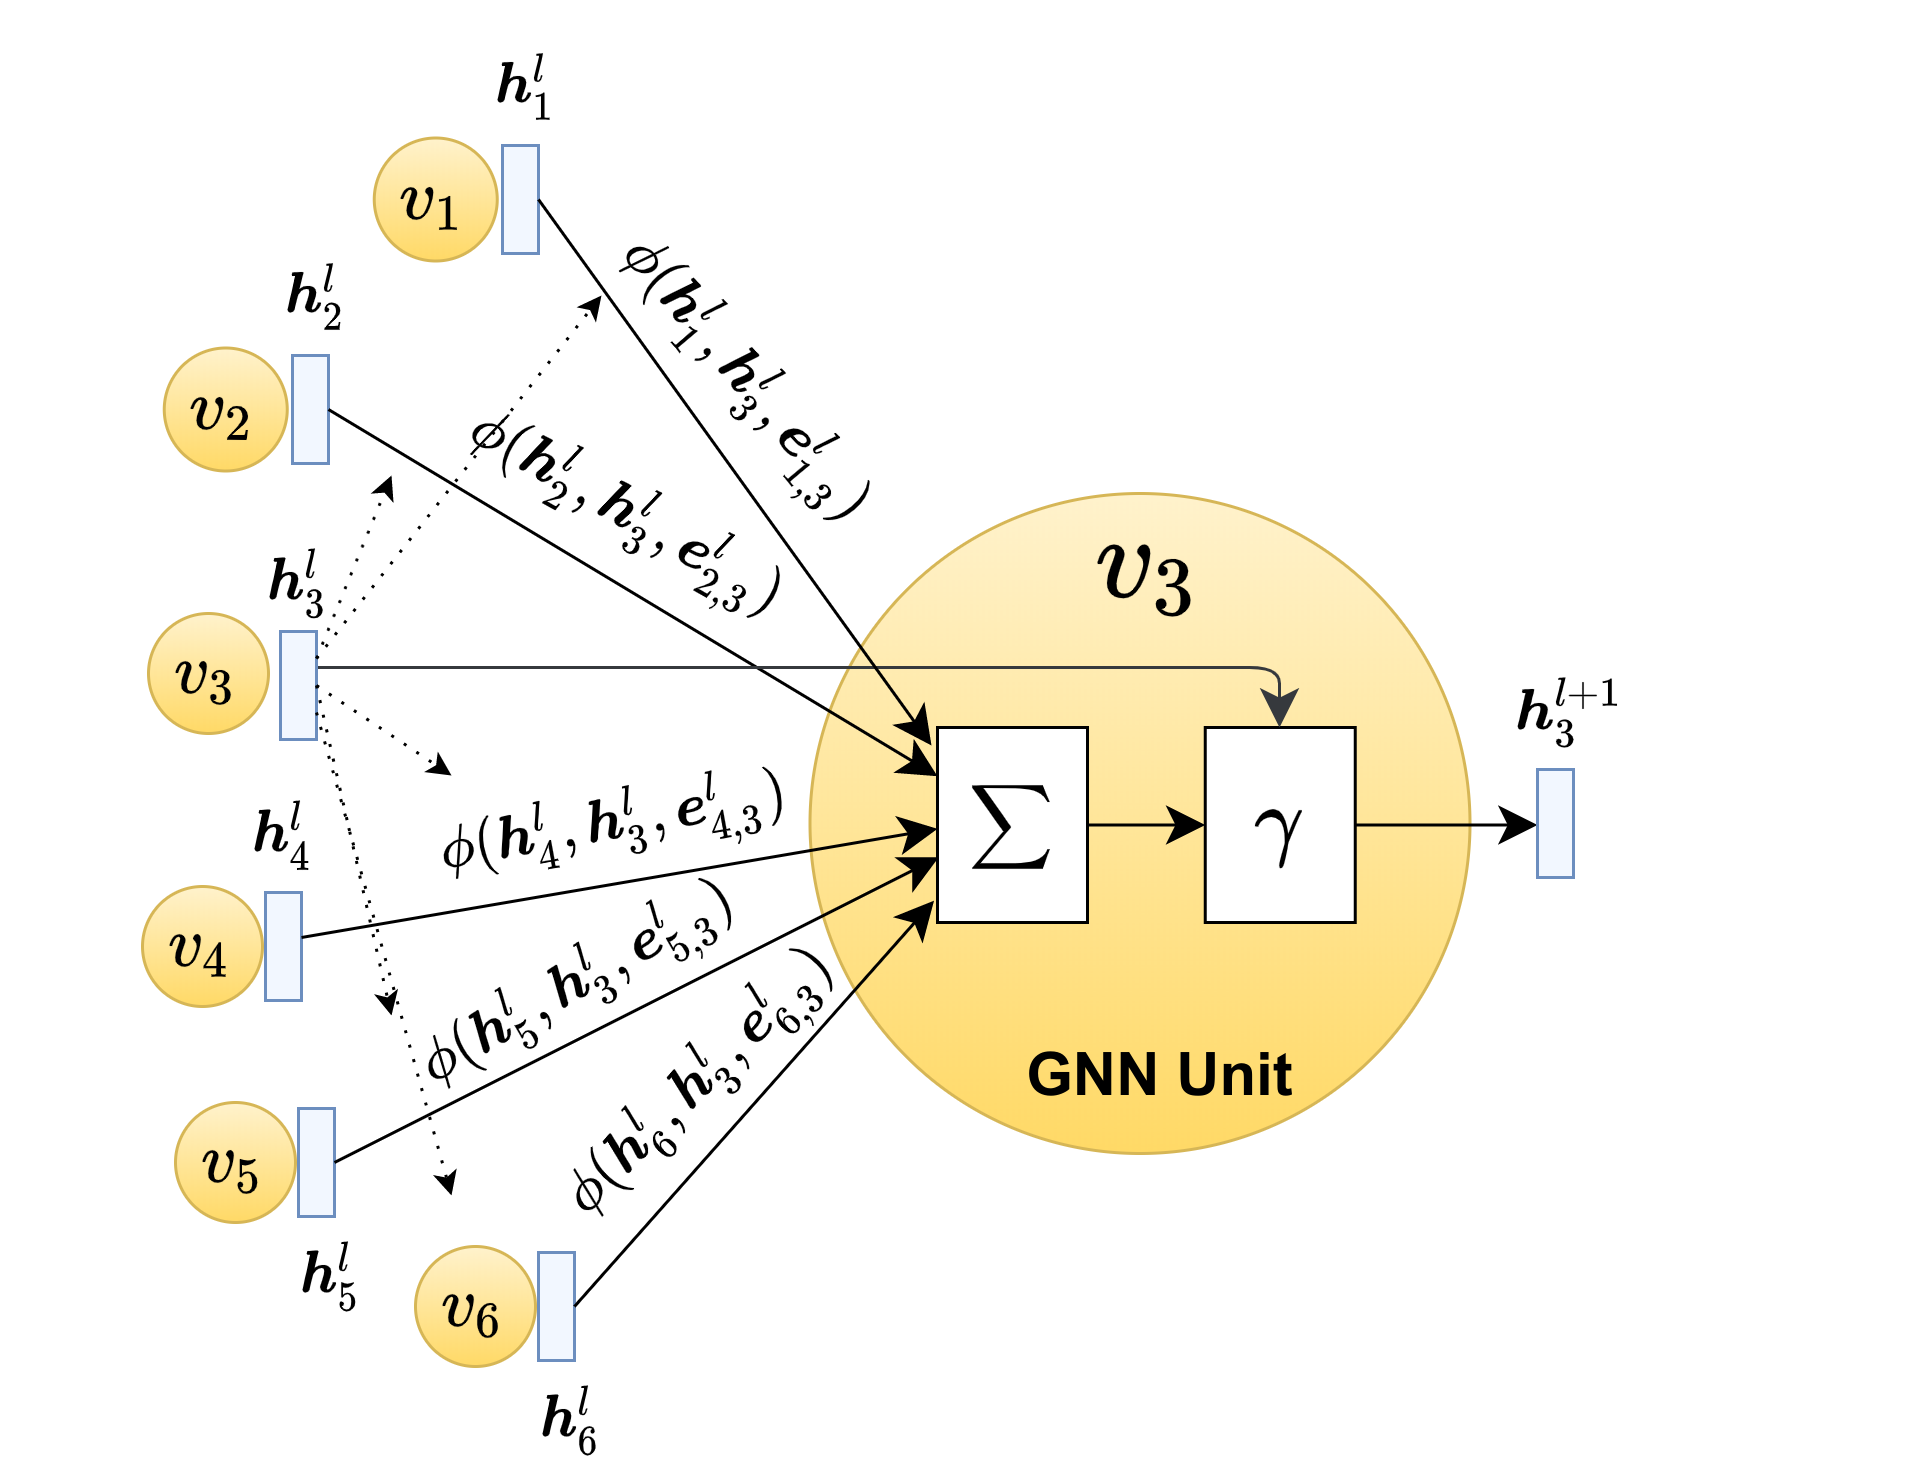
\includegraphics[width=0.5\columnwidth]{figs/illustration/GNN_Unit.png}
	\caption{Graph neuron of $v_3$ at the GNN layer $l$ with the graph $\mathcal{G}$ in \figurename~\ref{fig:general_structure_of_gnn}(b). $\phi$/$\Sigma$/$\gamma$ are the message/aggregation/vertex update functions in the message-passing model, respecitvely.}
	\label{fig:graph_neuron_structure}
\end{figure}

We follow the message-passing model \cite{gilmer_messgae_passing} to formally define a graph neuron.
The message-passing model is widely used in the cutting-edge GNN training systems like PyTorch Geometric (PyG) \cite{PyG} and Deep Graph Library (DGL) \cite{DGL}.
\figurename~\ref{fig:graph_neuron_structure} shows the structure of a graph neuron in the message-passing model.
A graph neuron collects messages from its neighbor graph neurons and outputs a hidden feature vector according to the aggregated messages.
Graph neurons at layer $l$ are made of three \emph{differentiable} functions: $\phi^l$, $\Sigma^l$ and $\gamma^l$.
The graph neuron calculates the output hidden vector $\boldsymbol{h}^{l+1}_i$ by
$$
	\boldsymbol{h}^{l+1}_i = \gamma^l(\boldsymbol{h}^l_i, \mathlarger{\Sigma}^l_{v_j \in \mathcal{N}(v_i)}{\phi^l(\boldsymbol{h}^l_i, \boldsymbol{h}^l_j,	\boldsymbol{e}_{j,i})}).
$$

$\phi^l$ is the \emph{message} function.
For every incident edge $(v_j, v_i)$ of $v_i$, $\phi$ receives the output hidden feature vectors $\boldsymbol{h}^l_i$ and $\boldsymbol{h}^l_j$ of the previous GNN layer and the edge feature vector $\boldsymbol{e}_{j,i}$ as the input.
$\phi^l$ emits a message vector $\boldsymbol{m}^l_{j,i}$ for every edge $(v_j, v_i)$ at layer $l$, i.e., $\boldsymbol{m}^l_{j,i}=\phi^l(\boldsymbol{h}^l_i, \boldsymbol{h}^l_j, \boldsymbol{e}_{j,i})$.
For $v_i$, the message vectors $\boldsymbol{m}^l_{x,j}$ of its adjacent edges ($v_x \in \mathcal{N}(v_i)$) are aggregated by the \emph{aggregation} function $\Sigma^l$ to produce an aggregated vector $\boldsymbol{s}^l_i$, i.e., $\boldsymbol{s}^l_i=\mathlarger{\Sigma}^l_{v_j \in \mathcal{N}(v_i)}\boldsymbol{m}^l_{j,i}$.
$v_i$'s aggregated vector $\boldsymbol{s}^l_i$ and its hidden vector $\boldsymbol{h}^l_i$ from the previous GNN layer are fed into the \emph{vertex update} function $\gamma^l$ to calculate the output hidden vector $\boldsymbol{h}^{l+1}_i$ of the current layer $l$, i.e., $\boldsymbol{h}^{l+1}_i = \gamma^l(\boldsymbol{h}^l_i, \boldsymbol{s}^l_i)$
The end-to-end training requires $\phi^l$ and $\gamma^l$ (like multi-layer perceptrons and GRU) and $\Sigma_l$ (like mean, sum, element-wise min/max) are \emph{differentiable} to make the whole GNN differentialble.

Different GNNs adopt different kinds of graph neurons and have different definitions of the three functions.
$\phi$ and $\Sigma$ are the \emph{edge calculation} functions.
They are conducted over every edge in $\mathcal{G}$.
$\gamma$ is the \emph{vertex calculation} function.
It is conducted over every vertex in $\mathcal{G}$.
\tablename~\ref{tab:gnn_overview_edge} and \tablename~\ref{tab:gnn_overview_vertex} list the edge functions and the vertex functions of typical GNNs, respectively.
For ChebNet, we report its GNN sub-layer in the tables. 
A ChebNet layer consists of $K$ GNN sub-layers and a summation layer:
$\boldsymbol{H}^{l+1} = \sum_{k=1}^K{\boldsymbol{Z}^{(k)} \textcolor{blue}{\boldsymbol{W}^{(k)}}}$ with the GNN sub-layers $\boldsymbol{Z}^{(1)}=\boldsymbol{H}^l$, $\boldsymbol{Z}^{(2)}=\hat{\boldsymbol{L}}\boldsymbol{H}^l$, and $\boldsymbol{Z}^{(k)}=2\hat{\boldsymbol{L}}\boldsymbol{Z}^{(k-1)} - \boldsymbol{Z}^{(k-2)}$, where $\boldsymbol{H}^l$ is the matrix of output hidden feature vectors of the layer $l-1$.
For GAT, a GAT layer consists of two sub-layers and it conducts part of the vertex calculation before the two sub-layers.
For GaAN, a GaAN layer consists of four sub-layers: the first sub-layer calculates the summation $\boldsymbol{m}_{j, i, (k)}^{l,0}  = \exp(\textcolor{blue}{FC_{\theta^{l, k}_{xa}}} (\boldsymbol{h}_j^l) \odot \textcolor{blue}{\boldsymbol{FC}_{\theta^{l,k}_{ya}}} (\boldsymbol{h}_i^l))$, and the other three layers calculate $\boldsymbol{m}^l_{j,i,1}$/$\boldsymbol{m}^l_{j,i,2}$/$\boldsymbol{m}^l_{j,i,3}$.

\begin{table}
	\hspace{-5em}
	\begin{footnotesize}
		\begin{tabular}{ccp{8em}p{22em}r}
			\toprule
			GNN                                                                                                                       &
			Type                                                                                                                      &
			$\Sigma$                                                                                                                  &
			$\phi$                                                                                                                    &
			Complexity                                                                                                                  \\ \midrule
			ChebNet \cite{defferrad2016_chebnet}                                                                                      &
			Spectral                                                                                                                  &
			sum                                                                                                                       &
			$\boldsymbol{m}_{j, i}^{(k)} = e_{j, i}\boldsymbol{z}_j^{(k-1)}$                                                          &
			$O(d_{in})$                                                                                                                 \\
			\textbf{GCN} \cite{kipf2017_gcn}                                                                                          &
			Spectral                                                                                                                  &
			sum                                                                                                                       &
			$\boldsymbol{m}_{j, i}^l = e_{j, i} \boldsymbol{h}_j^l$                                                                   &
			$O(d_{in})$                                                                                                                 \\
			AGCN                                                                                                                      &
			Spectral                                                                                                                  &
			sum                                                                                                                       &
			$\boldsymbol{m}_{j, i}^l = \tilde{e}_{j, i}^l \boldsymbol{h}_j^l$                                                         &
			$O(d_{in})$                                                                                                                 \\
			GraphSAGE                                                                                                                 &
			Non-spectral                                                                                                              &
			mean/LSTM                                                                                                                 &
			$\boldsymbol{m}_{j, i}^l =  \boldsymbol{h}_j^l$                                                                           &
			$O(1)$                                                                                                                      \\
			GraphSAGE-pool                                                                                                            &
			Non-spectral                                                                                                              &
			max                                                                                                                       &
			$\boldsymbol{m}_{j, i}^l =  \delta(\textcolor{blue}{\boldsymbol{W}^l_{pool}} \boldsymbol{h}_j^l + \textcolor{blue}{b}^l)$ &
			$O(d_{in} * d_{out})$                                                                                                       \\
			Neural FPs                                                                                                                &
			Non-spectral                                                                                                              &
			sum                                                                                                                       &
			$\boldsymbol{m}_{j, i}^l = \boldsymbol{h}_j^l$                                                                            &
			$O(1)$                                                                                                                      \\
			SSE                                                                                                                       &
			Recurrent                                                                                                                 &
			sum                                                                                                                       &
			$\boldsymbol{m}_{j, i}^l = [\boldsymbol{x}_j \parallel \boldsymbol{h}_j^l]$                                               &
			$O(f+d_{in})$                                                                                                               \\
			\textbf{GGNN}                                                                                                             &
			Gated                                                                                                                     &
			sum                                                                                                                       &
			$\boldsymbol{m}_{j, i} = \textcolor{blue}{\boldsymbol{W}^l} \boldsymbol{h}_j^l$                                           &
			$O(d_{in} * d_{out})$                                                                                                       \\
			\textbf{GAT}                                                                                                              &
			Attention                                                                                                                 &
			sum                                                                                                                       &
			\begin{scriptsize}
				$\begin{aligned}[t]
                         & \text{Sub-layer 0:}\\
                         & \boldsymbol{m}^{l,0}_{j,i,(k)} = \exp(LeakyReLU(\textcolor{blue}{\boldsymbol{a}^T} [\hat{\boldsymbol{h}}^{l}_{i,(k)} \parallel \hat{\boldsymbol{h}}^{l}_{j, (k)}]))\\
                         & \text{Sub-layer 1:}\\
						 & \alpha^l_{j, i, (k)} = \frac {\exp(LeakyReLU(\textcolor{blue}{\boldsymbol{a}^T} [\hat{\boldsymbol{h}}^{l}_{i,(k)} \parallel \hat{\boldsymbol{h}}^{l}_{j,(k)}] ))} {\hat{\boldsymbol{a}}^{l,0}_{i,(k)}} \\
						 & \text{Multi-head concatenation}: \boldsymbol{m}_{j, i}^{l,1} = \parallel_{k=1}^K \delta(\alpha^l_{j, i, (k)} \hat{\boldsymbol{h}}^{l}_{j,(k)})                                                                                                                                             \\
						 & \text{Multi-head average}: \boldsymbol{m}_{j, i}^{l,1} = \frac{1}{K} \sum_{k=1}^K \delta(\alpha^l_{j, i, (k)} \hat{\boldsymbol{h}}^{l}_{j,(k)})
					\end{aligned}$
			\end{scriptsize}
             &
             $
             \begin{aligned}[t]
                \text{concat: } O(d_{out}) &\\
                \text{average: } O(K * d_{out}) &\\
                \text{Two sub-layers} &
             \end{aligned}
             $ 
             \\
			\textbf{GaAN}                                                                                                             &
			Attention                                                                                                                 &
			sum,max,mean                                                                                                              &
			\begin{scriptsize}
				$\begin{aligned}[t]
						 & \text{Sub-layer 0:} \\
						 & \boldsymbol{m}_{j, i, (k)}^{l,0}  = \exp(\textcolor{blue}{FC_{\theta^{l, k}_{xa}}} (\boldsymbol{h}_j^l) \odot \textcolor{blue}{\boldsymbol{FC}_{\theta^{l,k}_{ya}}} (\boldsymbol{h}_i^l)) \\
						 & \text{Sub-layer 1:} \\
						 & \alpha^l_{j, i, (k)} = \frac {\exp(\textcolor{blue}{FC_{\theta^{l, k}_{xa}}} (\boldsymbol{h}_j^l) \odot \textcolor{blue}{\boldsymbol{FC}_{\theta^{l,k}_{ya}}} (\boldsymbol{h}_i^l))} {\hat{\boldsymbol{a}}^{l, 0}_{i, (k)}}\\
						 & \boldsymbol{m}_{j, i}^{l, 1} = \parallel_{k=1}^K \alpha_{j, i, (k)} \textcolor{blue}{\boldsymbol{FC}^h_{\theta^l_v}} \hat{\boldsymbol{h}}_{j, (k)}^l \\                                                                                                                                                                                                                                                                                           
						 & \text{Sub-layer 2:} \\
						 & \boldsymbol{m}_{j, i}^{l, 2} = \textcolor{blue}{\boldsymbol{FC}_{\theta^l_m}} \boldsymbol{h}_j^{l}  \\
						 & \text{Sub-layer 3:} \\
						 & \boldsymbol{m}_{j, i}^{l, 3} = \boldsymbol{h}_j^l
					\end{aligned}$
			\end{scriptsize}                                                                                            &
			\makecell[r]{$O(max(d_a, d_m, d_v) * K * d_{in})$ \\
                        Four sub-layers}\\
			\bottomrule
		\end{tabular}
	\end{footnotesize}
	\caption{Typical graph neural networks and their edge calculation functions.
		$d_{in}$ and $d_{out}$ are dimensions of the input and output hidden feature vectors, respectively.
		Blue variables are model parameters to learn. In GaAN, $FC^{\alpha}_{\theta}(x) = \alpha(\boldsymbol{W}\boldsymbol{x} + \boldsymbol{b})$, 
		where $\theta=\{\boldsymbol{W}, \boldsymbol{b}\}$, $\theta$ with different subscripts mean different transformation parameters, we denote $h(\cdot)$
		to be the $LeakyReLU$ for activation functions and $FC_{\theta}(x)$ means applying no activation function after the linear transform.
	}
	\label{tab:gnn_overview_edge}
\end{table}

\begin{table}
	\begin{footnotesize}
		\begin{tabular}{cp{20em}r}
			\toprule
			GNN                                                                                                                                                                                                              &
			$\gamma$                                                                                                                                                                                                         &
			Complexity                                                                                                                                                                                                         \\ \midrule
			ChebNet \cite{defferrad2016_chebnet}                                                                                                                                                                             &
			$\boldsymbol{z}_i^{(k)} = 2\boldsymbol{s}^{(k)}_{i} - \boldsymbol{z}_i^{(k-2)}$                                                                                                                                  &
			$O(d_{out})$                                                                                                                                                                                                       \\
			\textbf{GCN} \cite{kipf2017_gcn}                                                                                                                                                                                 &
			$\boldsymbol{h}_i^{l+1} = \textcolor{blue}{\boldsymbol{W}}^l  \boldsymbol{s}_i^{l}$                                                                                                                              &
			$O(d_{in} * d_{out})$                                                                                                                                                                                              \\
			AGCN                                                                                                                                                                                                             &
			$\boldsymbol{h}_i^{l+1} = \textcolor{blue}{\boldsymbol{W}}^l  \boldsymbol{s}_i^{l}$                                                                                                                              &
			$O(d_{in} * d_{out})$                                                                                                                                                                                              \\
			GraphSAGE                                                                                                                                                                                                        &
			$\boldsymbol{h}_i^{l+1} =   \delta(\textcolor{blue}{\boldsymbol{W}}^l  [\boldsymbol{s}_i^{l} \parallel \boldsymbol{h}_i^l])$                                                                                     &
			$O(d_{in} * d_{out})$                                                                                                                                                                                              \\
			GraphSAGE-pool                                                                                                                                                                                                   &
			$\boldsymbol{h}_i^{l+1} = \boldsymbol{s}_i^l$                                                                                                                                                                    &
			$O(1)$                                                                                                                                                                                                             \\
			Neural FPs                                                                                                                                                                                                       &
			$\boldsymbol{h}_i^{l+1} = \delta(\textcolor{blue}{\boldsymbol{W}}^{l, |\mathcal{N}(i)|}  (\boldsymbol{h}_i^l + \boldsymbol{s}_i^{l}))$                                                                           &
			$O(d_{in} * d_{out})$                                                                                                                                                                                              \\
			SSE                                                                                                                                                                                                              &
			$\boldsymbol{h}_i^{l+1} = (1 - \alpha)  \boldsymbol{h}_i^l +\alpha    \delta(\textcolor{blue}{\boldsymbol{W}}^l_1 \delta(\textcolor{blue}{\boldsymbol{W}}^l_2 [\boldsymbol{x}_i \parallel \boldsymbol{s}_i^l]))$ &
			$O((f + d_{in}) * d_{out})$                                                                                                                                                                                        \\
			\textbf{GGNN}                                                                                                                                                                                                    &
			\begin{scriptsize}
				$\begin{aligned}[t]
						 & {\boldsymbol{z}}_i^l = \delta ( \textcolor{blue}{\boldsymbol{W}}^z \boldsymbol{s}_i^l + \textcolor{blue}{\boldsymbol{b}}^{sz} + \textcolor{blue}{\boldsymbol{U}}^z \boldsymbol{h}_i^{l} + \textcolor{blue}{\boldsymbol{b}}^{hz})                    \\
						 & \boldsymbol{r}_i^l = \delta ( \textcolor{blue}{\boldsymbol{W}}^r \boldsymbol{s}_i^l+ \textcolor{blue}{\boldsymbol{b}}^{sr} +\textcolor{blue}{\boldsymbol{U}}^r \boldsymbol{h}_i^{l} + \textcolor{blue}{\boldsymbol{b}}^{hr})                        \\
						 & \boldsymbol{h}_i^{l+1} = tanh ( \textcolor{blue}{\boldsymbol{W}} \boldsymbol{s}_i^l + \textcolor{blue}{\boldsymbol{b}}^s + \textcolor{blue}{\boldsymbol{U}} ( \boldsymbol{r}_i^l \odot \boldsymbol{h}_i^{l}) + \textcolor{blue}{\boldsymbol{b}}^h)) \\
						 & \boldsymbol{h}_i^{l+1} = (1 - {\boldsymbol{z}}_i^l) \odot \boldsymbol{h}_i^l + {\boldsymbol{z}}_i^l \odot \boldsymbol{h}_i^{l+1}
					\end{aligned}$
			\end{scriptsize}
			                                                                                                                                                                                                                 &
			$O(d_{in} * d_{out})$                                                                                                                                                                                              \\
			\textbf{GAT} &
            \begin{scriptsize}
                $\begin{aligned}[t]
                & \text{Preprocessing:}\\
                & \hat{\boldsymbol{h}}^{l}_{i,(k)} = \textcolor{blue}{\boldsymbol{W}^{l,k}} \boldsymbol{h}_i^{l}\\
                & \text{Sub-layer 0:}\\
                & \hat{\boldsymbol{a}}^{l,0}_{i,(k)} = \boldsymbol{s}^{l,0}_{i,(k)}\\
                & \text{Sub-layer 1:}\\
                & \boldsymbol{h}_i^{l+1} = \boldsymbol{s}_i^{l,1}
                \end{aligned}
                $
            \end{scriptsize} &
             $
             \begin{aligned}[t]
             \text{concat:} O(d_{in}*d_{out}) &\\
             \text{average:} O(K*d_{in}*d_{out}) &\\
             \text{Two sub-layers}&
            \end{aligned}
             $
           \\
			\textbf{GaAN}                                                                                                                                                                                                    &
			\begin{scriptsize}
				$\begin{aligned}[t]
						& \text{Sub-layer 0:}\\
						& \hat{\boldsymbol{a}}^{l,0}_{i,(k)} = \boldsymbol{s}^{l,0}_{i,(k)}\\
						& \text{Sub-layer 1,2,3:}\\
						& \boldsymbol{g}_i^l = \textcolor{blue}{\boldsymbol{FC}_{\theta^l_g}}(\boldsymbol{h}_i^{l} \parallel \boldsymbol{s}_{i}^{l, 2} \parallel \boldsymbol{s}_{i}^{l, 3}) \\
						& \boldsymbol{h}_i^{l+1} = \textcolor{blue}{\boldsymbol{FC}_{\theta^l_o}} (\boldsymbol{h}_i^l \parallel (\boldsymbol{g}_{i}^l \odot \boldsymbol{s}_{i}^{l, 1}))
					\end{aligned}$
			\end{scriptsize}                                                                                                                                                                                   &
			\makecell[r]{$O(max(K * d_v + d_{in}, 2 * d_{in} + d_m) * d_{out})$\\
                         Four sub-layers}
            \\ \bottomrule
		\end{tabular}
	\end{footnotesize}
	\caption{Typical graph neural networks and their vertex calculation functions.
		$d_{in}$ and $d_{out}$ are dimensions of the input and output hidden feature vectors, respectively.
		Blue variables are model parameters to learn.
		In Neural FPs, $\textcolor{blue}{\boldsymbol{W}}^{l, |\mathcal{N}(i)|}$ is the weight matrix for vertices with degree $|\mathcal{N}(i)|$ at layer $l$. 
		In GaAN, $FC^{\alpha}_{\theta}(x) = \alpha(\boldsymbol{W}\boldsymbol{x} + \boldsymbol{b})$, 
		where $\theta=\{\boldsymbol{W}, \boldsymbol{b}\}$, $\theta$ with different subscripts mean different transformation parameters, we denote $h(\cdot)$
		to be the $LeakyReLU$ for activation functions and $FC_{\theta}(x)$ means applying no activation function after the linear transform.}
	\label{tab:gnn_overview_vertex}
\end{table}

\subsection{Classification of GNNs}

Since we focus on analyzing the performance bottleneck in training GNNs, we classify the typical GNNs from the view of time complexity.
We use $O_\phi$/$O_\Sigma$/$O_\gamma$ to denote the time complexity of the three functions in the message-passing model.
The time complexity of a GNN layer is made up of two parts: the edge calculation complexity $m * (O_\phi$ + $O_\Sigma)$ and the vertex calculation complexity $n * O_\gamma$.

In \tablename~\ref{tab:gnn_overview_edge} and \tablename~\ref{tab:gnn_overview_vertex}, we list the edge and vertex calculation complexity, respectively.
The time complexity of a graph neuron are affected by the dimensions of the input/output hidden vectors $d_{in}$ and $d_{out}$ and the dimensions of the model parameters (like the number of heads $K$ in GAT and the dimensions of the view vectors $d_a$/$d_v$ in GaAN).

We classify the typical GNNs into four quadrants based on their edge/vertex complexity as shown in \figurename~\ref{fig:gnn_complexity_quadrant}. We pick GCN, GGNN, GAT and GaAN as the \emph{representative GNNs} of the four quadrants.

\begin{figure}
	\centering
	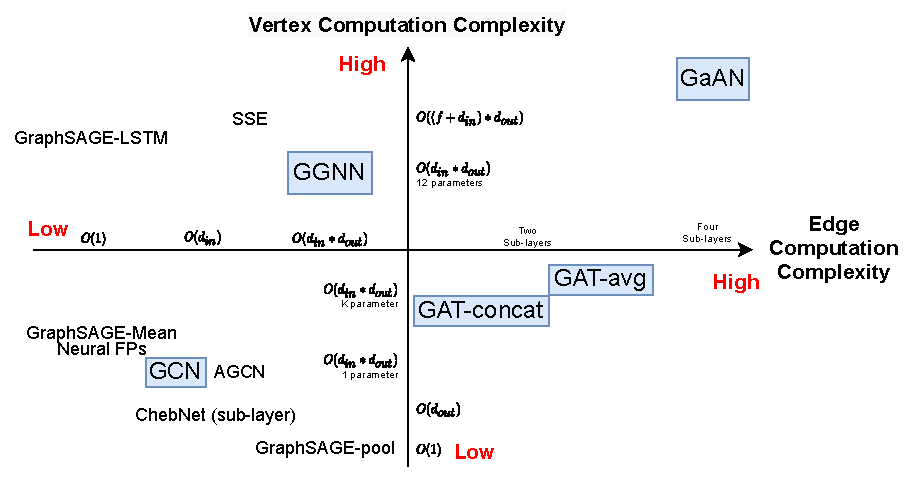
\includegraphics[width=0.7\columnwidth]{figs/illustration/GNN_complexity_quadrant.pdf}
	\caption{Complexity quadrants of typical GNNs. We compare the complexity according to the number of sub-layers, the Big-O notation and the number of parameters to train.}
	\label{fig:gnn_complexity_quadrant}
\end{figure}

\textbf{GCN} \cite{kipf2017_gcn} (low vertex \& edge calculation complexity): Graph convolution network (GCN) is the first-order approximation of the spectral-based graph convolutions.
%By combining the advantages of both the spectral-based and the spatial-based convolution, it can learn the representation of the local topological structure and vertex features efficiently.
It has only one parameter to learn at each layer, i.e. the weight matrix $\boldsymbol{W}^l$ in $\gamma$.
A GCN graph neuron can be expressed as $\boldsymbol{h}^{l+1}_i = \boldsymbol{W}^l\sum_{v_j \in \mathcal{N}(v_i)}{e_{j,i}\boldsymbol{h}^l_j}$, where $e_{j,i}$ is the normalized weight of the edge $(v_j, v_i)$.
%In the matrix view, $\boldsymbol{H}^{l+1} = (\boldsymbol{A}\boldsymbol{H}^l)\boldsymbol{W}^l$.
According to the associative law of the matrix multiplication, $\boldsymbol{h}^{l+1}_i = \sum_{v_j \in \mathcal{N}(v_i)}{e_{j,i}\boldsymbol{W}^l\boldsymbol{h}^l_j}$.
Since the dimension of $\boldsymbol{h}^{l+1}_i$ is usually smaller than $\boldsymbol{h}^l_i$ in practical GCNs, the implementation of GCN in PyTorch Geometric chooses to first conduct the vertex calculation $\hat{\boldsymbol{h}}^l_j = \boldsymbol{W}^l\boldsymbol{h}^l_j$ for each vertex $v_j$ and then conduct the edge calculation $\boldsymbol{h}^{l+1}_i=\sum_{v_j\in\mathcal{N}(v_i)}{e_{j,i}\hat{\boldsymbol{h}}^l_j}$.
As $\hat{\boldsymbol{h}}^l_j$ has the same dimension as $\boldsymbol{h}^{l+1}_i$, the implementation significantly reduces the  computation cost of the edge calculation.

\textbf{GGNN} (high vertex \& low edge calculation complexity):
GGNN introduces the gated recurrent unit (GRU) into the graph neural networks.
The vertex update function $\phi$ of GGNN is a modified GRU unit that has 12 model parameters to learn, having high computational complexity.
To lower the training cost, all GNN layers share the same group of parameters in GGNN.
GGNN further requires the dimension of $\boldsymbol{h}^{l+1}$ is equal to the dimension of $\boldsymbol{h}^l$.
Since the message function $\phi$ only uses the hidden feature vector $\boldsymbol{h}^l_j$ of the source vertex $v_j$ of an edge $(v_j, v_i)$, in the implementation, GGNN conducts the pre-processing vertex calculation $\hat{\boldsymbol{h}}^l_i=\boldsymbol{W}\boldsymbol{h}^l_i$ for every vertex $v_i$ before the message-passing.
The message function $\phi$ directly uses $\hat{\boldsymbol{h}}^l_j$ as the message vector for the edge $(v_j, v_i)$. 
By this way, GGNN further reduces the time complexity of the edge calculation to $O(1)$ without increasing the time complexity of the vertex calculation. 

\textbf{GAT} (low vertex \& high edge calculation complexity):
GAT introduces the attention and multi-head mechanism into the graph neural networks.
The $K$ heads generate $K$ independent views for an edge, where $K$ is a hyper-parameter.
The views of $K$ heads can be merged by concatenating or by averaging.
For concatenating, the dimension of the hidden feature vector of each head $d_{head}$ is $d_{out}/K$.
For averaging, $d_{head}$ is $d_{out}$, multiplying the complexity by $K$.
Each GAT layer consists of a preprocessing step and two sub-layers.
In the preprocessing step, GAT calculates the attention vectors $\hat{\boldsymbol{h}}^{l}_{i,(k)}$ for every vertex $v_i$ in every head $k$.
The first sub-layer uses the attention vectors to calculate the attention weights of every edge in every head $\boldsymbol{m}^{l,0}_{j,i,(k)}$.
After the message-passing, the first-layer gets the summation of attention weights of every vertex in every head $\hat{\boldsymbol{a}}^{l,0}_{i,(k)}$.
The second sub-layer gets the normalized attention weights $\alpha_{j, i, (k)}$ for every edge in every head and aggregates the hidden feature vectors with the normalized weights in the message-passing.
GAT uses the aggreated vector $\boldsymbol{s}^{l,1}_i$ of the second sub-layer as the output hidden vector directly.

\textbf{GaAN} (high vertex \& edge calculation complexity):
Based on the multi-head machanism, GaAN introduces a convolutional subnetwork to control the weight of each head. Different to multi-head machanism in GAT, GaAN project the center vertex feature to the query vector (dimension is $d_v$) and
the neighboring vertex features are projected to get key and value vectors. The dimension of key and values vectors are the same, we set to $d_a$.
$K$ is the number of attention heads. The weight of each head is calculated by a convolutional network, which takes the feature of each vertex and its neighbors as input to get the gated values with number of $K$. 
The convolutional network is built by combining average pooling and max pooling. Moreover, the max pooling needs to project the vertex feature to a transformed vector with dimension of $d_m$, costing an additional computational overhead.
Each GaAN layer consists of four sub-layers. The first sub-layer aims to get the summation of attention weights of every vertex in each head.
The second sub-layer uses to aggreate neighboring vertices's query vector with the normalized attention weights $\alpha_{j, i, (k)}$ for every head. 
And the third sub-layer is used in max-pooling and it gets the element-wise max vector of neighboring vertices' transformed vectors by message-passing.
The last sub-layer gets element-wise mean vector of neighboring vertices' vectors by message-passing. The gate values $\boldsymbol{g}^l_i$ is obtained by using a fully-connected layer with vector concatenating $\boldsymbol{h}^{l}_i$, $\boldsymbol{s}^{l, 2}_i$ and $\boldsymbol{s}^{l, 3}_i$.
At last, GaAN uses a fully-connected layer with concatenating $\boldsymbol{h}^{l}_i$ and the result of element-wise multiplying $\boldsymbol{g}^{l}_i$ and $\boldsymbol{s}^{l, 0}_i$ to get the output hidden vector.

\subsection{Sampling Techniques}

By default, GNNs are trained in a full-batch way, using the whole graph in each iteration.
The full-batch gradient descent has two disadvantages \cite{chiang2019_cluster_gcn}.
It has to cache intermediate results of all vertices in the forward phase, which consumes lots of memory space.
It updates the parameters only once for each epoch, slowing the convergence of gradient descent.

To train GNNs in a mini-batch way, several sampling techniques are proposed.
In each mini-batch, they sample a small subgraph from the whole graph $\mathcal{G}$ and uses the subgraph to update the model parameters.
In other words, the sampling techniques only active the graph neurons and the connections that appear in the sampled subgraph between GNN layers, as shown in \figurename~\ref{fig:gnn_sampling}.
Inactive graph neurons and connetions do not participate in the training of this mini-batch, saving lots of computation and storage costs.
Moreover, it may reduce the risk of overfitting the training graph.
Based on whether different GNN layers sample different subgraphs, the existing sampling techniques can be devided into two groups \cite{zeng2020_graphsaint}: the neighbor sampling and the graph sampling.

The neighbor sampling techniques \cite{hamilton2017_graphsage, ying2018_pinsage, chen2018_fastgcn, chen2018_sgcn, huang2018_adap} sample the subgraphs layer by layer.
They first sample several vertices from $\mathcal{V}$ in the last GNN layer.
Then they repeatedly sample the neighbors of those vertices in the previous layer until the input layer.
The sampled subgraphs of different GNN layers may be \emph{different}, as shown in \figurename~\ref{fig:gnn_sampling_neighbor_sampling}.
GraphSAGE \cite{hamilton2017_graphsage} is the representative technique.
For every sampled vertex $v_i$ in the GNN layer $l$, GraphSAGE samples at most $S^l$ neighbors of $v_i$ in the previous GNN layer.
$S^l$ is the hyperparameter that is usually much smaller than $|\mathcal{V}|$.
By this way, GraphSAGE limits the neighborhood sizes of the vertices in the sampled subgraph, especially high-degree vertices.

\begin{figure}
	\centering
	\subfloat[Neighbor sampling\label{fig:gnn_sampling_neighbor_sampling}]{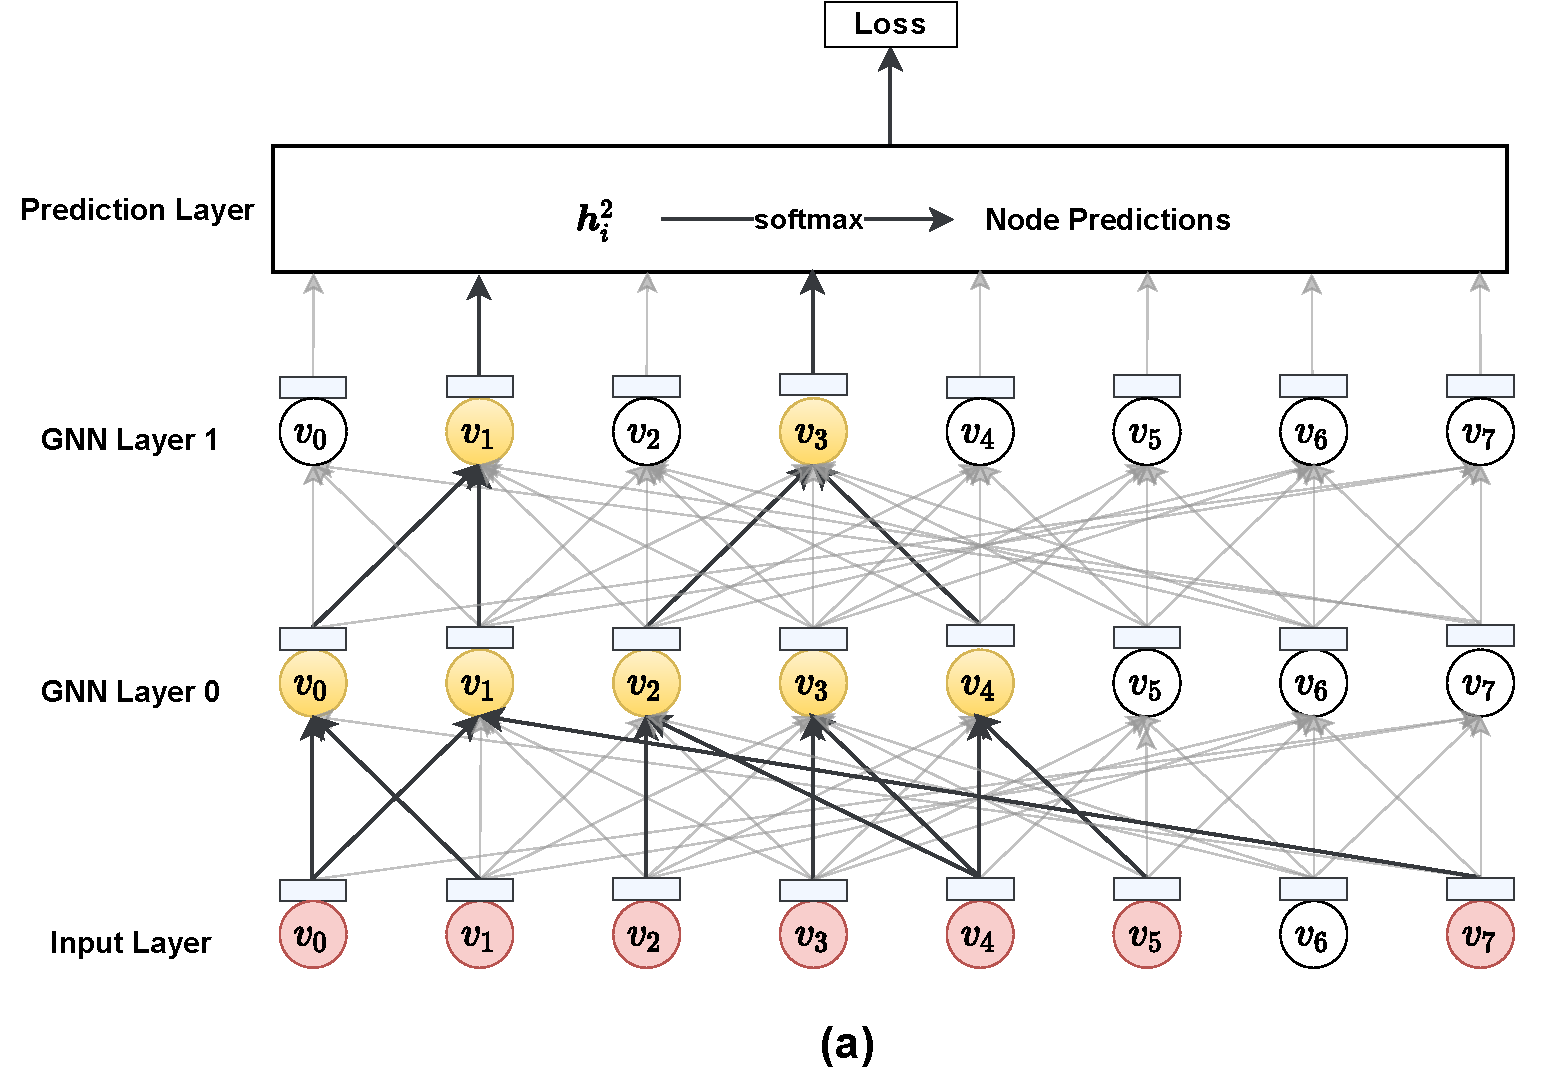
\includegraphics[height=4cm]{figs/illustration/layer_sampling.pdf}}
	%
	\subfloat[Graph sampling\label{fig:gnn_sampling_graph_sampling}]{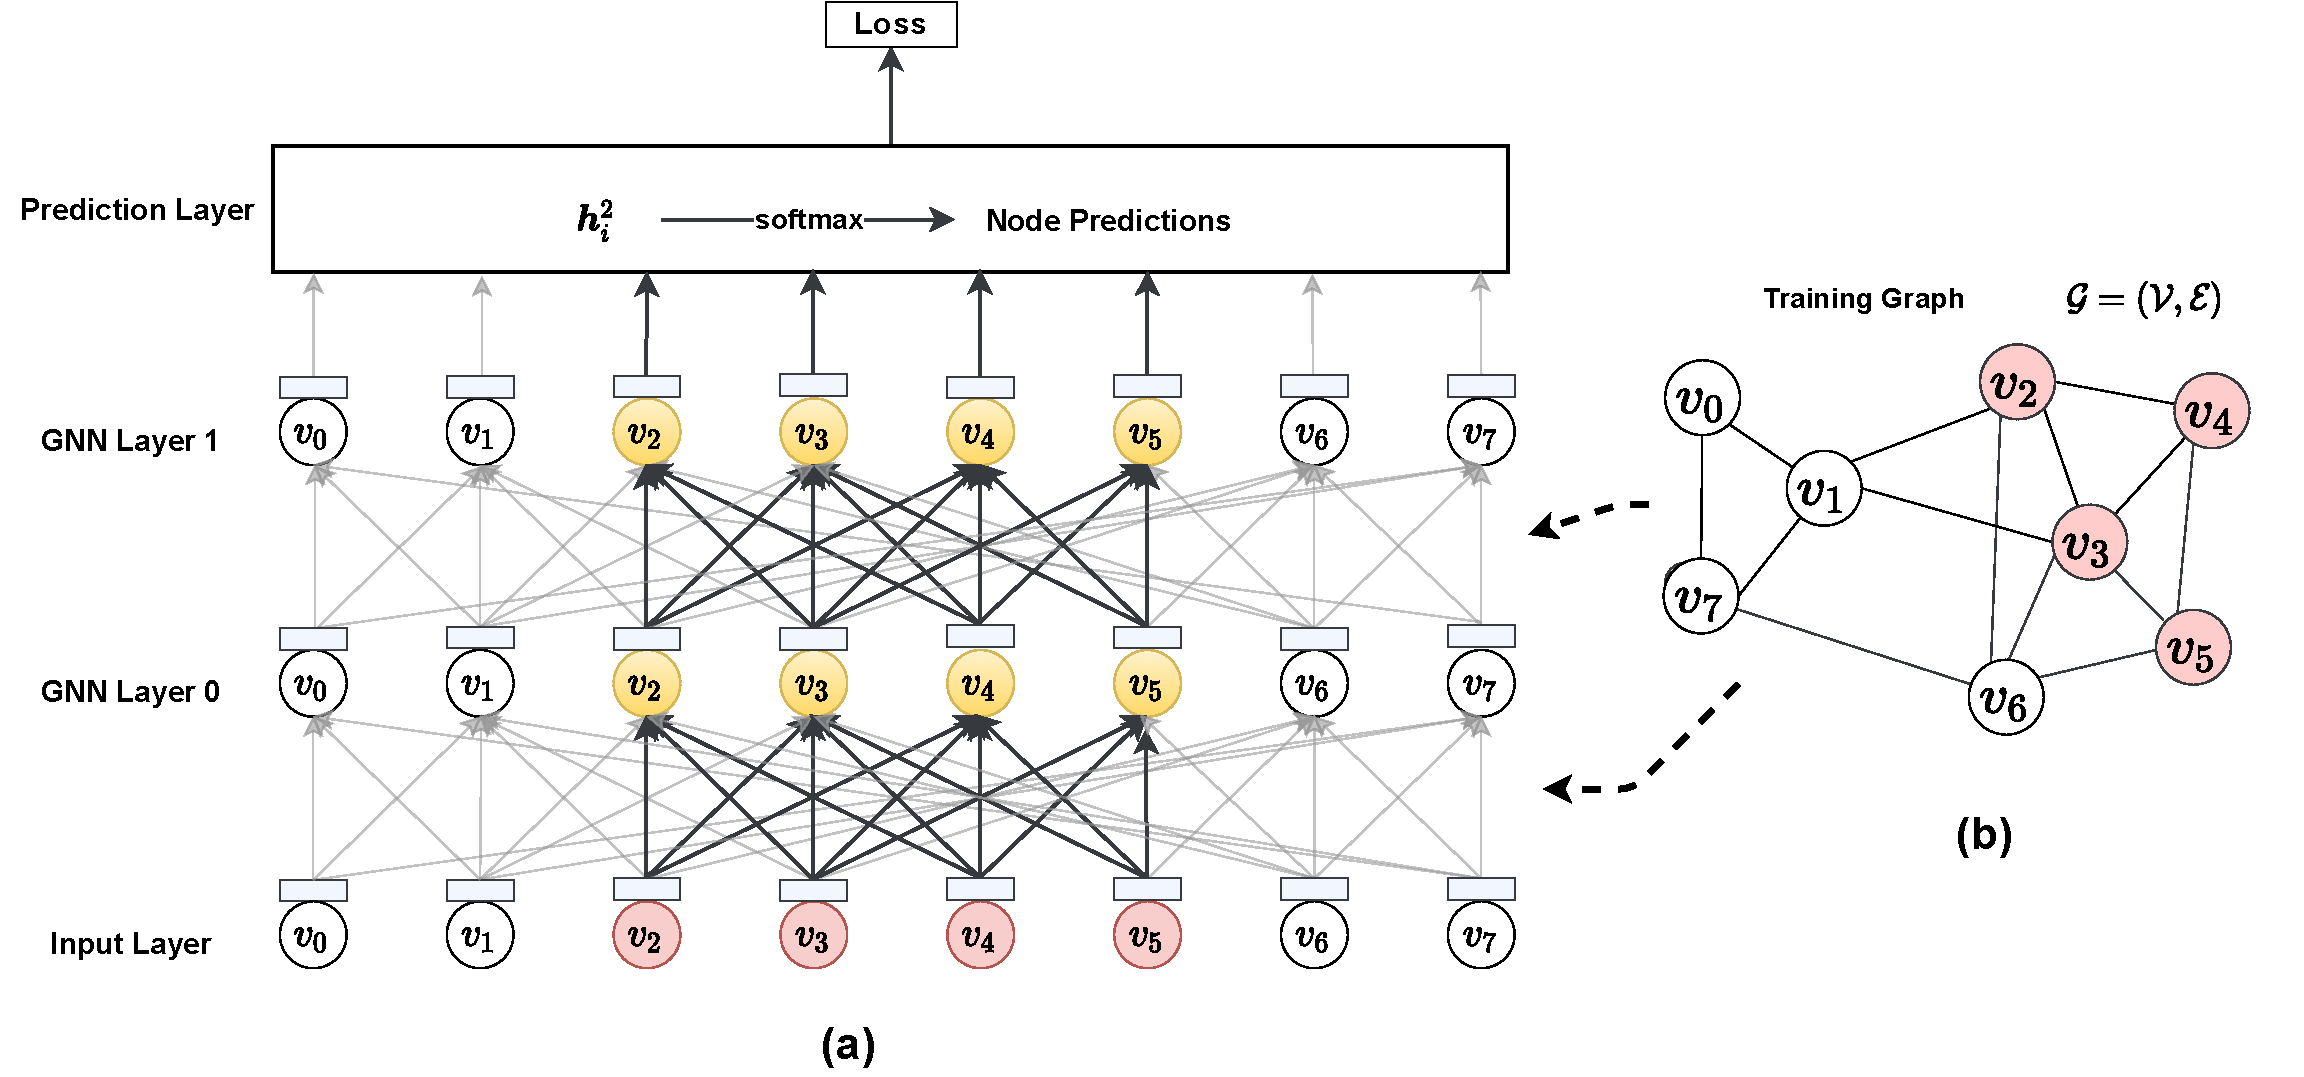
\includegraphics[height=4cm]{figs/illustration/graph_sampling.pdf}}
	\caption{Training a GNN with sampling techniques. The faded graph neurons and their connections are inactivated.}
	\label{fig:gnn_sampling}
\end{figure}

The graph sampling techniques \cite{zeng2018_aesg, chiang2019_cluster_gcn, zeng2020_graphsaint} sample a subgraph for each mini-batch and use the same sampled graph for all GNN layers, as shown in \figurename~\ref{fig:gnn_sampling_graph_sampling}.
They differ in the methods to sample subgraphs.
The cluster sampler technique \cite{chiang2019_cluster_gcn} is the representative technique.
Given a training graph $\mathcal{G}$, it partitions $\mathcal{G}$ into closely connected clusters.
For each mini-batch, it randomly picks $K$ clusters, where $K$ is the hyperparameter.
The technique ignores the inter-cluster edges and only keeps the intra-cluster edges in the subgraph.


\section{Evaluation Design}
\label{sec:experimental_design}

We design a series of experiments to explore the performance bottleneck in training graph neural networks.
We first introduce the experimental setting in Section~\ref{sec:experimental_env} and then give out our experimental scheme in Section~\ref{sec:experimental_scheme}.
The evaluation results are presented and analyzed later in Section~\ref{sec:experiment_results}.

\subsection{Experimental Setting}
\label{sec:experimental_env}

\paragraph{Experimental Environment}
All the experiments were conducted in a CentOS 7 Linux server with kernel version 3.10.0.
The server had 40 cores and 90 GB main memory.
The server was equipped with an NVIDIA Tesla T4 GPU with 16GB GDDR6 memory.
For the software environment, we adopted Python 3.7.7, PyTorch 1.5.0, and CUDA 10.1.
We implemented all the GNNs with PyTorch Geometric 1.5.0.

\paragraph{Dataset}
We used six real-world graph datasets as listed in \tablename~\ref{tab:dataset_overview} that were popular in the GNN accuracy evaluation \cite{yang2016_revisiting_semisupervised, zeng2020_graphsaint, shchur2018_pitfall_of_gnn}.
For directed graphs, PyG converts them into undirected ones during the data loading.
Thus, the average degree of a directed graph $\bar{d}=\frac{2|\mathcal{E}|}{|\mathcal{V}|}$.
For an undirected graph, $\mathcal{E}$ already contains two-direction edges and $\bar{d}=\frac{|\mathcal{E}|}{|\mathcal{V}|}$.
For the \texttt{cam} dataset, we generated random dense feature vectors.
We also used random graphs generated by the R-MAT graph generator \cite{rmat-generator} in the experiments, to explore the effects of graph topological characteristics (like the average degree) on the performance bottleneck.
Input feature vectors of random graphs were random dense vectors with a dimension of 32.
Vertices of random graphs were classified into 10 classes randomly.

\begin{table}
    \centering
    \begin{tabular}{cccccccc}
        \toprule
        Dataset                                                 & $|\mathcal{V}|$ & $|\mathcal{E}|$ & $\bar{d}$ & $dim(\boldsymbol{x})$ & \#Class & Directed \\
        \midrule
        pubmed (pub) \cite{yang2016_revisiting_semisupervised}  & 19,717          & 44,324          & 4.5       & 500                   & 3       & Yes      \\
        amazon-photo (amp) \cite{shchur2018_pitfall_of_gnn}     & 7,650           & 119,081         & 31.1      & 745                   & 8       & Yes      \\
        amazon-computers (amc) \cite{shchur2018_pitfall_of_gnn} & 13,752          & 245,861         & 35.8      & 767                   & 10      & Yes      \\
        coauthor-physics (cph) \cite{shchur2018_pitfall_of_gnn} & 34,493          & 247,962         & 14.4      & 8415                  & 5       & Yes      \\
        flickr (fli) \cite{zeng2020_graphsaint}                 & 89,250          & 899,756         & 10.1      & 500                   & 7       & No       \\
        com-amazon (cam) \cite{yang2012_defining}               & 334,863         & 925,872         & 2.8       & 32                    & 10      & No       \\
        \bottomrule
    \end{tabular}
    \caption{Dataset overview. $\bar{d}$ represents the average vertex degree. $dim(\boldsymbol{x})$ is the dimension of the input feature vector.}
    \label{tab:dataset_overview}
\end{table}

\paragraph{Learning Task}
We used the node classification as the target task in GNNs due to its popularity in real-world applications.
We trained GNNs with the semi-supervised learning setting.
All vertices and their input feature vectors were used, but only parts of the vertices were attached with labels during the training and they were used to calculate the loss and gradients.
The vertices with unseen labels were used in the evaluation phase to evaluate the accuracy of the current parameters.
%Since model parameters of GNNs were not restricted by the topological structure of $\mathcal{G}$, the model learned from the semi-supervised learning can directly extrapolate to unseen vertices.

\paragraph{GNN Implementation}
We implemented the four typical GNNs (GCN, GGNN, GAT, GaAN) with PyTorch Geometric 1.5.0.
To compare the performance characteristics of four GNNs side-by-side, we used a unified GNN structure for them: Input Layer $\rightarrow$ GNN Layer 0 $\rightarrow$ GNN Layer 1 $\rightarrow$ Softmax Layer (to prediction).
The structure was popular in the experimental evaluation of GCN \cite{kipf2017_gcn}, GAT \cite{huang2018_gat} and GaAN \cite{zhang2018_gaan}.
Since a GGNN layer requires the input and output hidden feature vectors have the same dimension, we added two multi-layer perceptron(MLP) layers to transform the dimensions of the input/output feature vectors of the whole GNN: Input Layer $\rightarrow$ MLP $\rightarrow$ GGNN Layer 0 $\rightarrow$ GGNN Layer 1 $\rightarrow$ MLP $\rightarrow$ Softmax Layer.
We stored the dataset and the model parameters on the GPU side.
All the training was conducted on the GPU.

\paragraph{Hyper-parameters}
We use $dim(\boldsymbol{v})$ to denote the dimension of a vector $\boldsymbol{v}$.
We picked the hyper-parameters of GNNs according to their popularity in the original papers.
We used the same set of hyper-parameters for all the datasets. 
Some hyper-parameters like the dimensions of hidden feature vectors were common in the four GNNs and we set them to the same values.
For GCN/GAT/GaAN, we set $\boldsymbol{h}^0_i = \boldsymbol{x}_i$, $dim(\boldsymbol{h}^1_i)=64$, and $dim(\boldsymbol{h}^2_i)=\#Classes$.
For GAT, we set the hyper-parameters according to \cite{huang2018_gat}.
The first GAT layer had 8 heads with the dimension of each head $d^0_{head}=8$. The first GAT layer merged the heads by concatenating.
The second GAT layer used a single head with the dimension $d^1_{head}=d^1_{out}=\#Classes$.
For GGNN, since it uses extra MLP layers to transform the dimensions of the input/output feature vectors, we set $dim(\boldsymbol{h}^0_i) = dim(\boldsymbol{h}^1_i) = dim(\boldsymbol{h}^2_i) = 64$.
We used 8 heads in the both GaAN layers with $d_a=d_v=8$ and $d_m=64$.

\paragraph{Sampling Techniques}

We picked the neighbor sampler from GraphSAGE \cite{hamilton2017_graphsage} and the cluster sampler from ClusterGCN \cite{chiang2019_cluster_gcn} as the typical sampling techniques respectively.
For the neighbor sampler, we set the neighborhood sample sizes as 25 for GNN Layer 1, and 10 for GNN Layer 0 and set the default batch size as 512 from \cite{hamilton2017_graphsage}.
For the cluster sampler, we partitioned every input graph into 1500 partitions and used 20 partitions per batch according to \cite{chiang2019_cluster_gcn}.

\subsection{Experimental Scheme}
\label{sec:experimental_scheme}

To find out the performance bottleneck in GNN training, we conducted the experimental analysis with four questions.
The answers to those questions will give us a more comprehensive view of the performance characteristics of GNN training.

\begin{itemize}

    \item[Q1] \emph{How do the hyper-parameters affect the training time and the memory usage of a GNN?} (Section~\ref{sec:effects_of_hyper-parameters_on_performance})

          Every GNN has a group of hyper-parameters like the number of GNN layers and the dimensions of hidden feature vectors. The hyper-parameters affect the training time per epoch and the peak memory usage during the training.
          To evaluate their effects, we measured how the training time per epoch and the peak memory usage (of the GPU) changed as we increased the values of the hyper-parameters.
          Through the experiments, we want to verify the validity of the computational complexity analysis in \tablename~\ref{tab:gnn_overview_edge} and \tablename~\ref{tab:gnn_overview_vertex}.
          If the complexity analysis is valid, we can analyze the bottleneck theoretically.

    \item[Q2] \emph{Which stage is the most time-consuming stage in GNN training?} (Section~\ref{sec:training_time_breakdown})

          We can decompose the training time on different levels: layer level, edge/vertex calculation level, and the basic operator level.
          On each level, we decomposed the training time of an epoch into several stages. The most time-consuming stage is the performance bottleneck.
          Optimizing its implementation can significantly reduce the training time.

    \item[Q3] \emph{Which consumes most of memory in GNN training?} (Section~\ref{sec:memory_usage_analysis})

          The limited memory capacity of a GPU is the main factor preventing us from training GNNs on big graphs.
          We measured the peak memory usage of GNN training under different graph scales, input feature dimensions, and average vertex degrees.
          Based on the results, we analyzed which is the most memory-consuming component in a GNN.
          Reducing its memory usage will enable us to train GNNs on bigger graphs under the same memory capacity.

    \item[Q4] \emph{Can the sampling techniques remove the performance bottleneck in GNN training?} (Section~\ref{sec:effects_of_sampling_techniques_on_performance})

          Theoretically, the sampling techniques can significantly reduce the number of graph neurons that participate in the training of a batch.
          Consequently, the training time and the memory usage should also decrease.
          To validate the effectiveness of the sampling techniques, we measured the training time and peak memory usage under different batch sizes.
          If the sampling techniques are effective, they are the keys to conduct GNN training on very big graphs.
          If they are not effective, we want to find out which impairs its efficiency.
\end{itemize}


\section{Evaluation Results and Analysis}
\label{sec:experiment_results}

We answer the four questions in Section~\ref{sec:experimental_scheme} one by one with experiments.
%
Without otherwise mentioned, the reported training time per epoch was the average wall-clock training time of 50 epochs, excluding abnormal epochs.
%
During the training of some epochs, there were extra profiling overheads from NVIDIA Nsight Systems and GC pauses from the Python interpreter that significantly increased the training time.
%
We denoted the 25\% and 75\% quantiles of the training time of 50 epochs as Q1 and Q3, respectively.
%
We regarded the epochs with the training time \emph{outside} the range of $[Q1 - 1.5 * (Q3-Q1), Q3 + 1.5 * (Q3-Q1)]$ as abnormal epochs.

\subsection{Effects of Hyper-parameters on Performance}
\label{sec:effects_of_hyper-parameters_on_performance}

The hyper-parameters of a GNN (such as the dimensions of hidden vectors and the number of heads) determined the model complexity of the GNN.
%
They affected the training/inference time, memory usage, and accuracy of the GNN at the same time.


\paragraph{Effects on Training/Inference Time}

According to \tablename~\ref{tab:gnn_overview_edge} and \tablename~\ref{tab:gnn_overview_vertex}, the time complexity of the messaging function $\phi^l$ and the updating function $\gamma^l$ are linear to each hyper-parameter separately.
%
If we increase one of the hyper-parameters and fix the others, the training/inference time should increase linearly in theory.

To verify the time complexity analysis in \tablename~\ref{tab:gnn_overview_edge} and \tablename~\ref{tab:gnn_overview_vertex}, we first compared the training time of the four GNNs in \figurename~\ref{fig:exp_absolute_training_time}.
%
The ranking of the training time was GaAN $\gg$ GAT $>$ GGNN $>$ GCN in all cases.
%
Since the real-world graphs had more edges than vertices ($|\mathcal{E}| > |\mathcal{V}|$), the time complexity of the edge calculation stage affected more than the vertex calculation stage.
%
The ranking was consistent with the time complexity analysis.

\begin{figure}[htb]
    \centering
    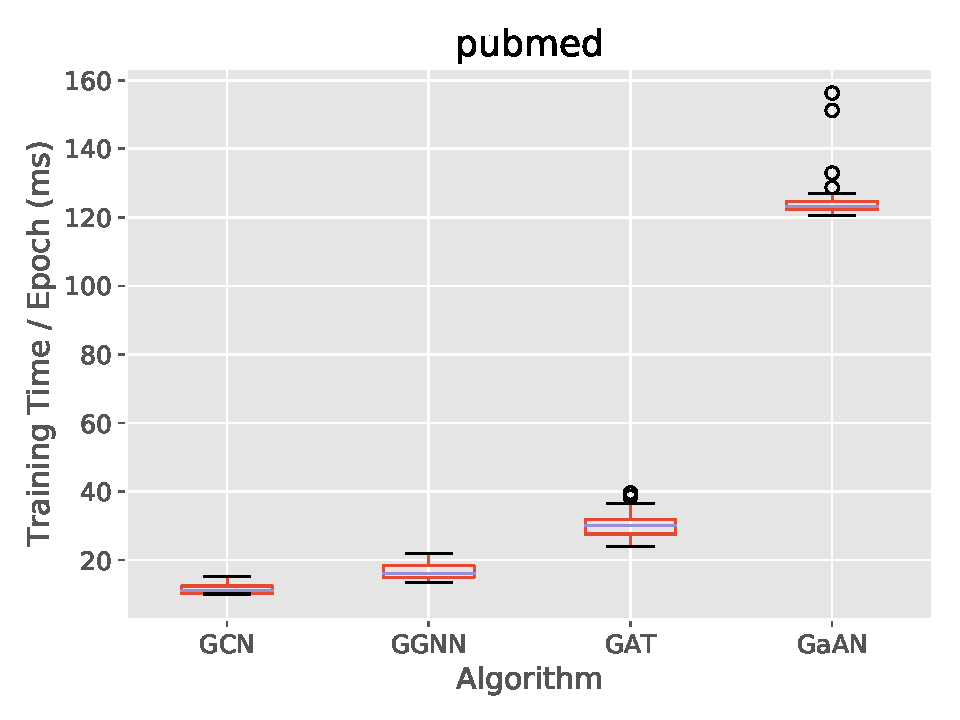
\includegraphics[width=0.3\textwidth]{figs/experiments/exp_absolute_training_time_comparison_pubmed.pdf}
    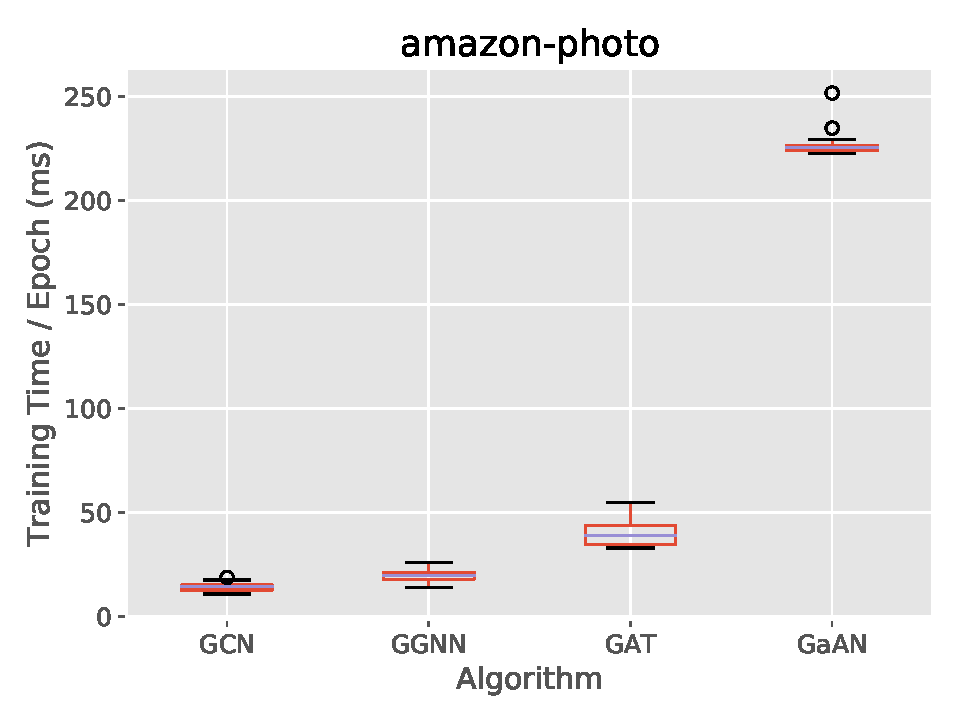
\includegraphics[width=0.3\textwidth]{figs/experiments/exp_absolute_training_time_comparison_amazon-photo.pdf}
    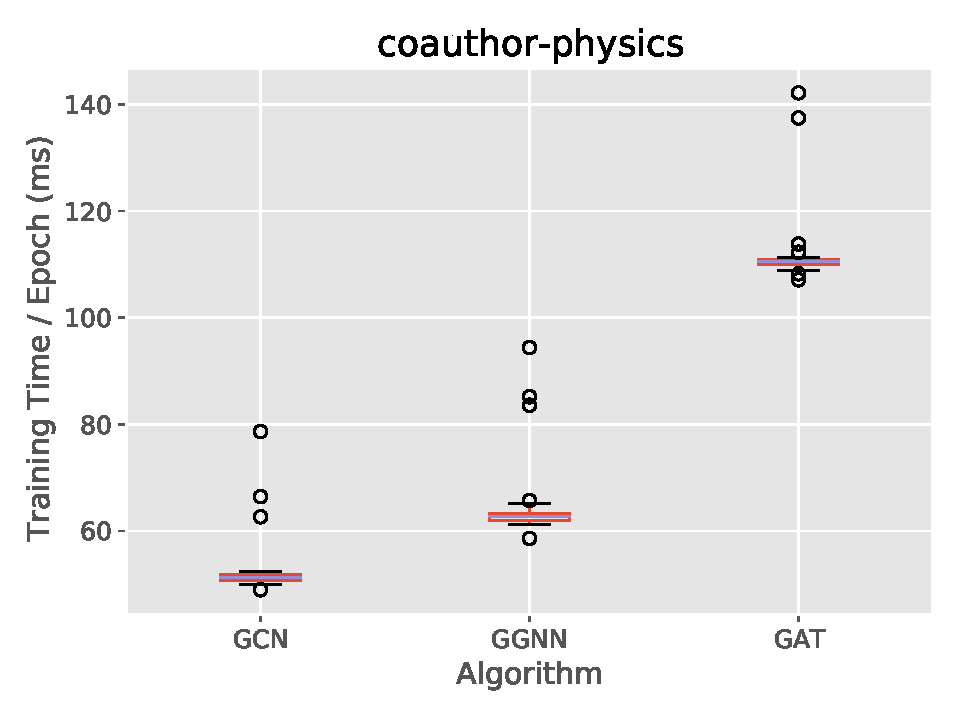
\includegraphics[width=0.3\textwidth]{figs/experiments/exp_absolute_training_time_comparison_coauthor-physics.pdf}

    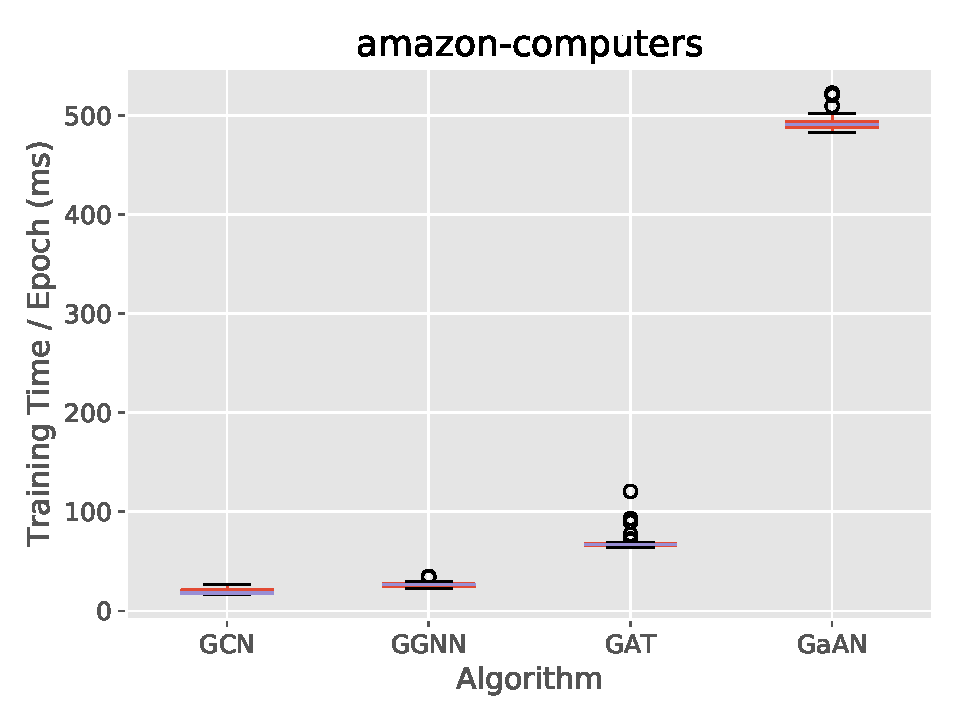
\includegraphics[width=0.3\textwidth]{figs/experiments/exp_absolute_training_time_comparison_amazon-computers.pdf}
    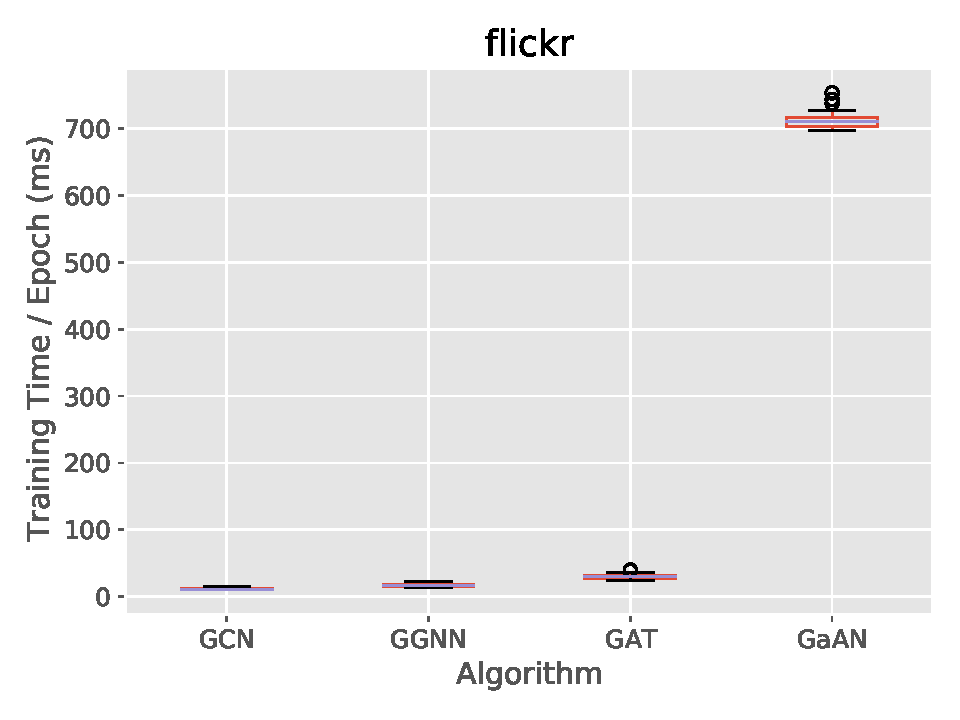
\includegraphics[width=0.3\textwidth]{figs/experiments/exp_absolute_training_time_comparison_flickr.pdf}
    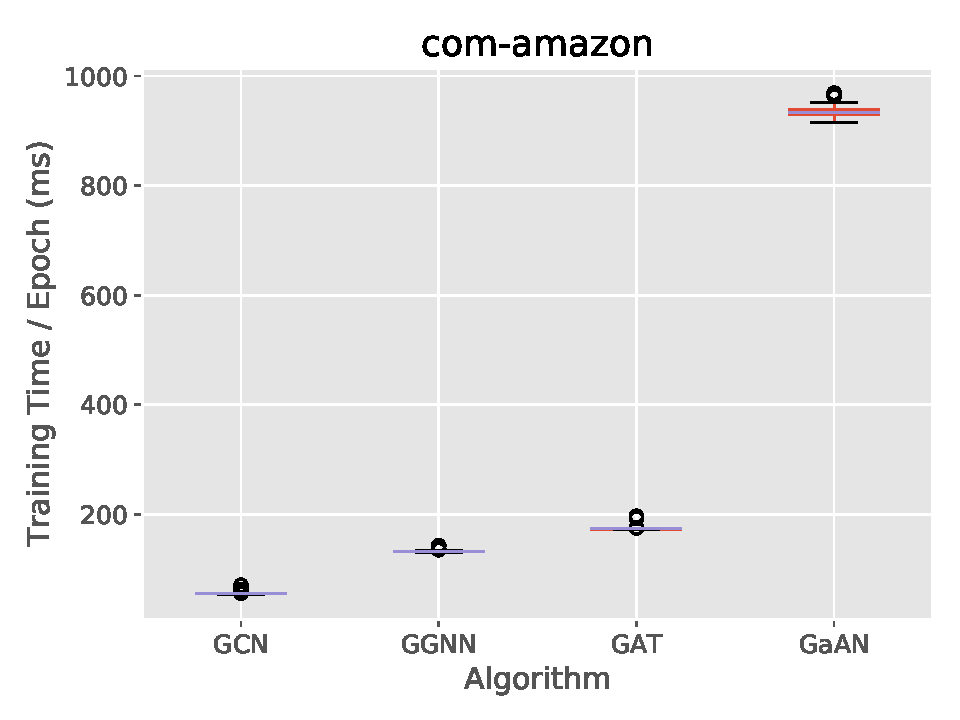
\includegraphics[width=0.3\textwidth]{figs/experiments/exp_absolute_training_time_comparison_com-amazon.pdf}
    \caption{Distribution of the wall-clock training time of 50 epoches on different datasets. GaAN crashed due to out of memory exception on the \texttt{cph} dataset.}
    \label{fig:exp_absolute_training_time}
\end{figure}

To further evaluate effects of hyper-parameters on training time, we measured the training time of each GNN with varying hyper-parameters in \figurename~\ref{fig:exp_hyperparameter_on_vertex_edge_phase_time_gcn} to \figurename~\ref{fig:exp_hyperparameter_on_vertex_edge_phase_time_gaan}.

\begin{figure}[H]
    \centering
    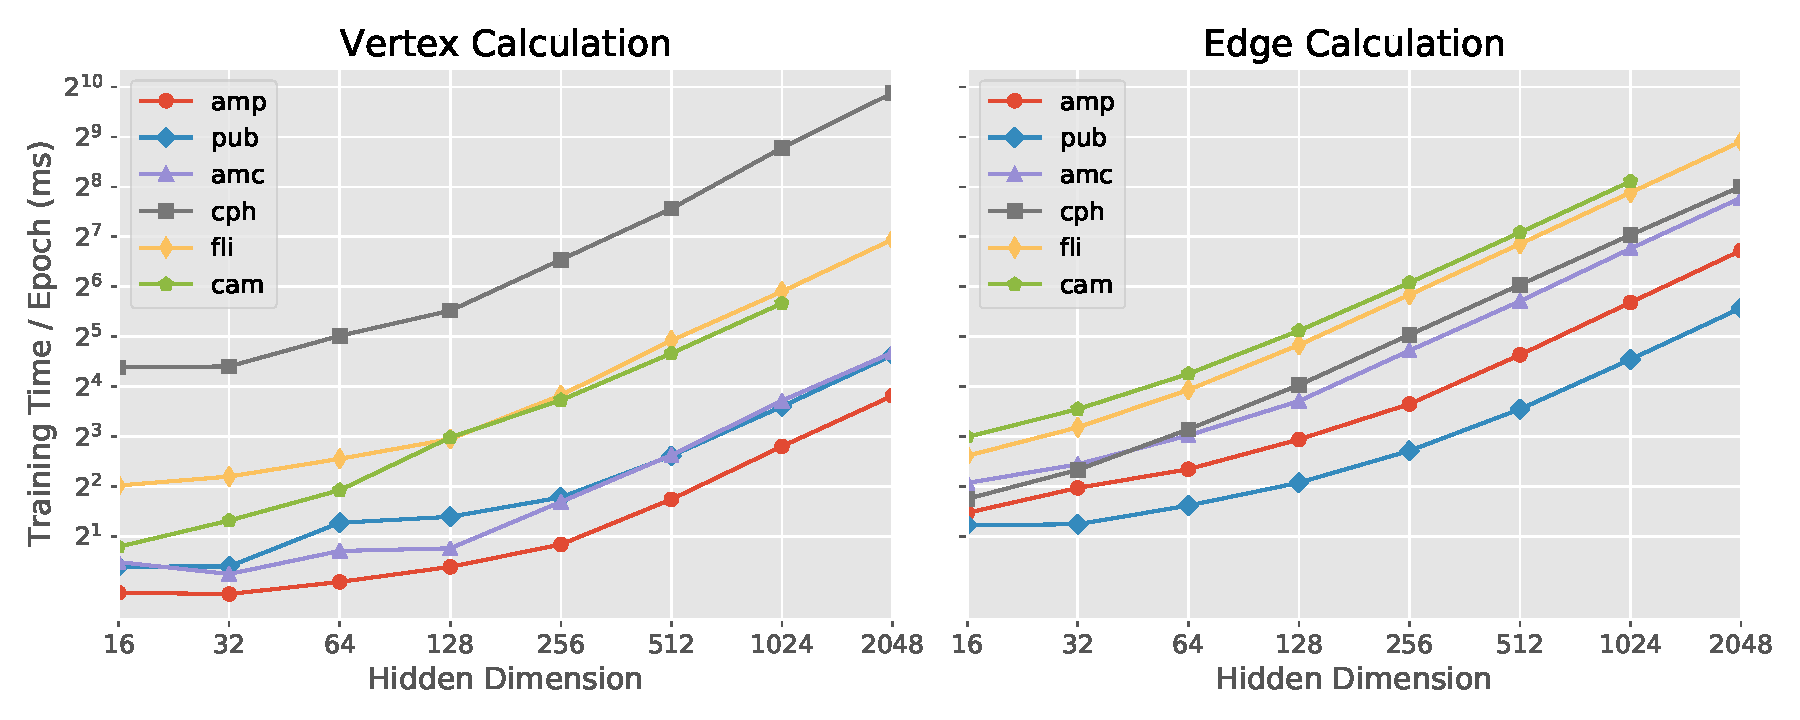
\includegraphics[width=0.6\textwidth]{figs/experiments/exp_hyperparameter_on_vertex_edge_phase_time_gcn.pdf}
    \caption{Effects of hyper-parameters on the vertex/edge calculation time of GCN.}
    \label{fig:exp_hyperparameter_on_vertex_edge_phase_time_gcn}
\end{figure}

\begin{figure}[H]
    \centering
    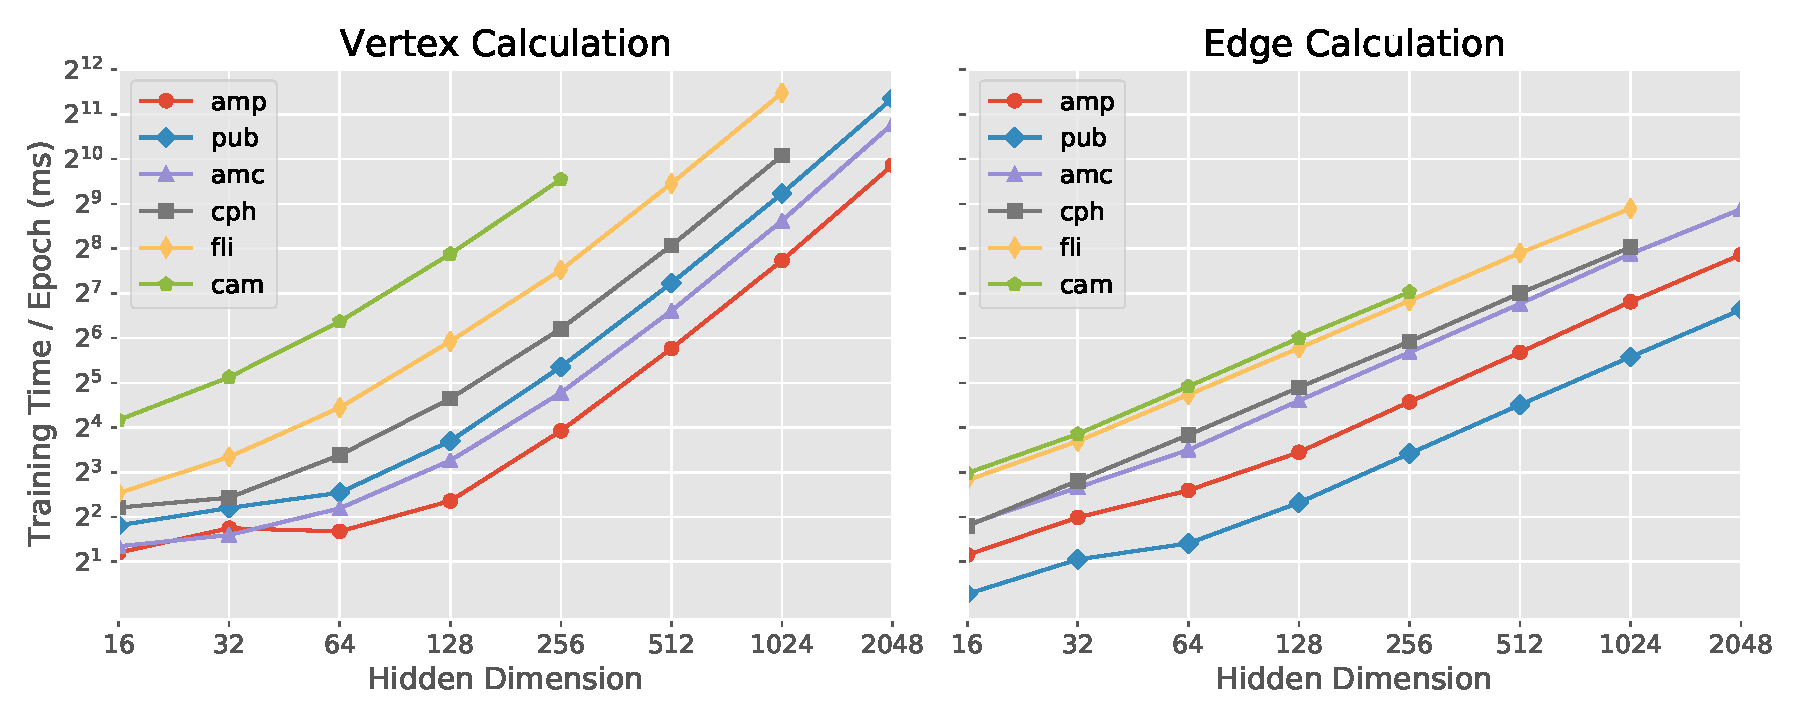
\includegraphics[width=0.6\textwidth]{figs/experiments/exp_hyperparameter_on_vertex_edge_phase_time_ggnn.pdf}
    \caption{Effects of hyper-parameters on the vertex/edge calculation time of GGNN.}
    \label{fig:exp_hyperparameter_on_vertex_edge_phase_time_ggnn}
\end{figure}

\begin{figure}[H]
    \centering
    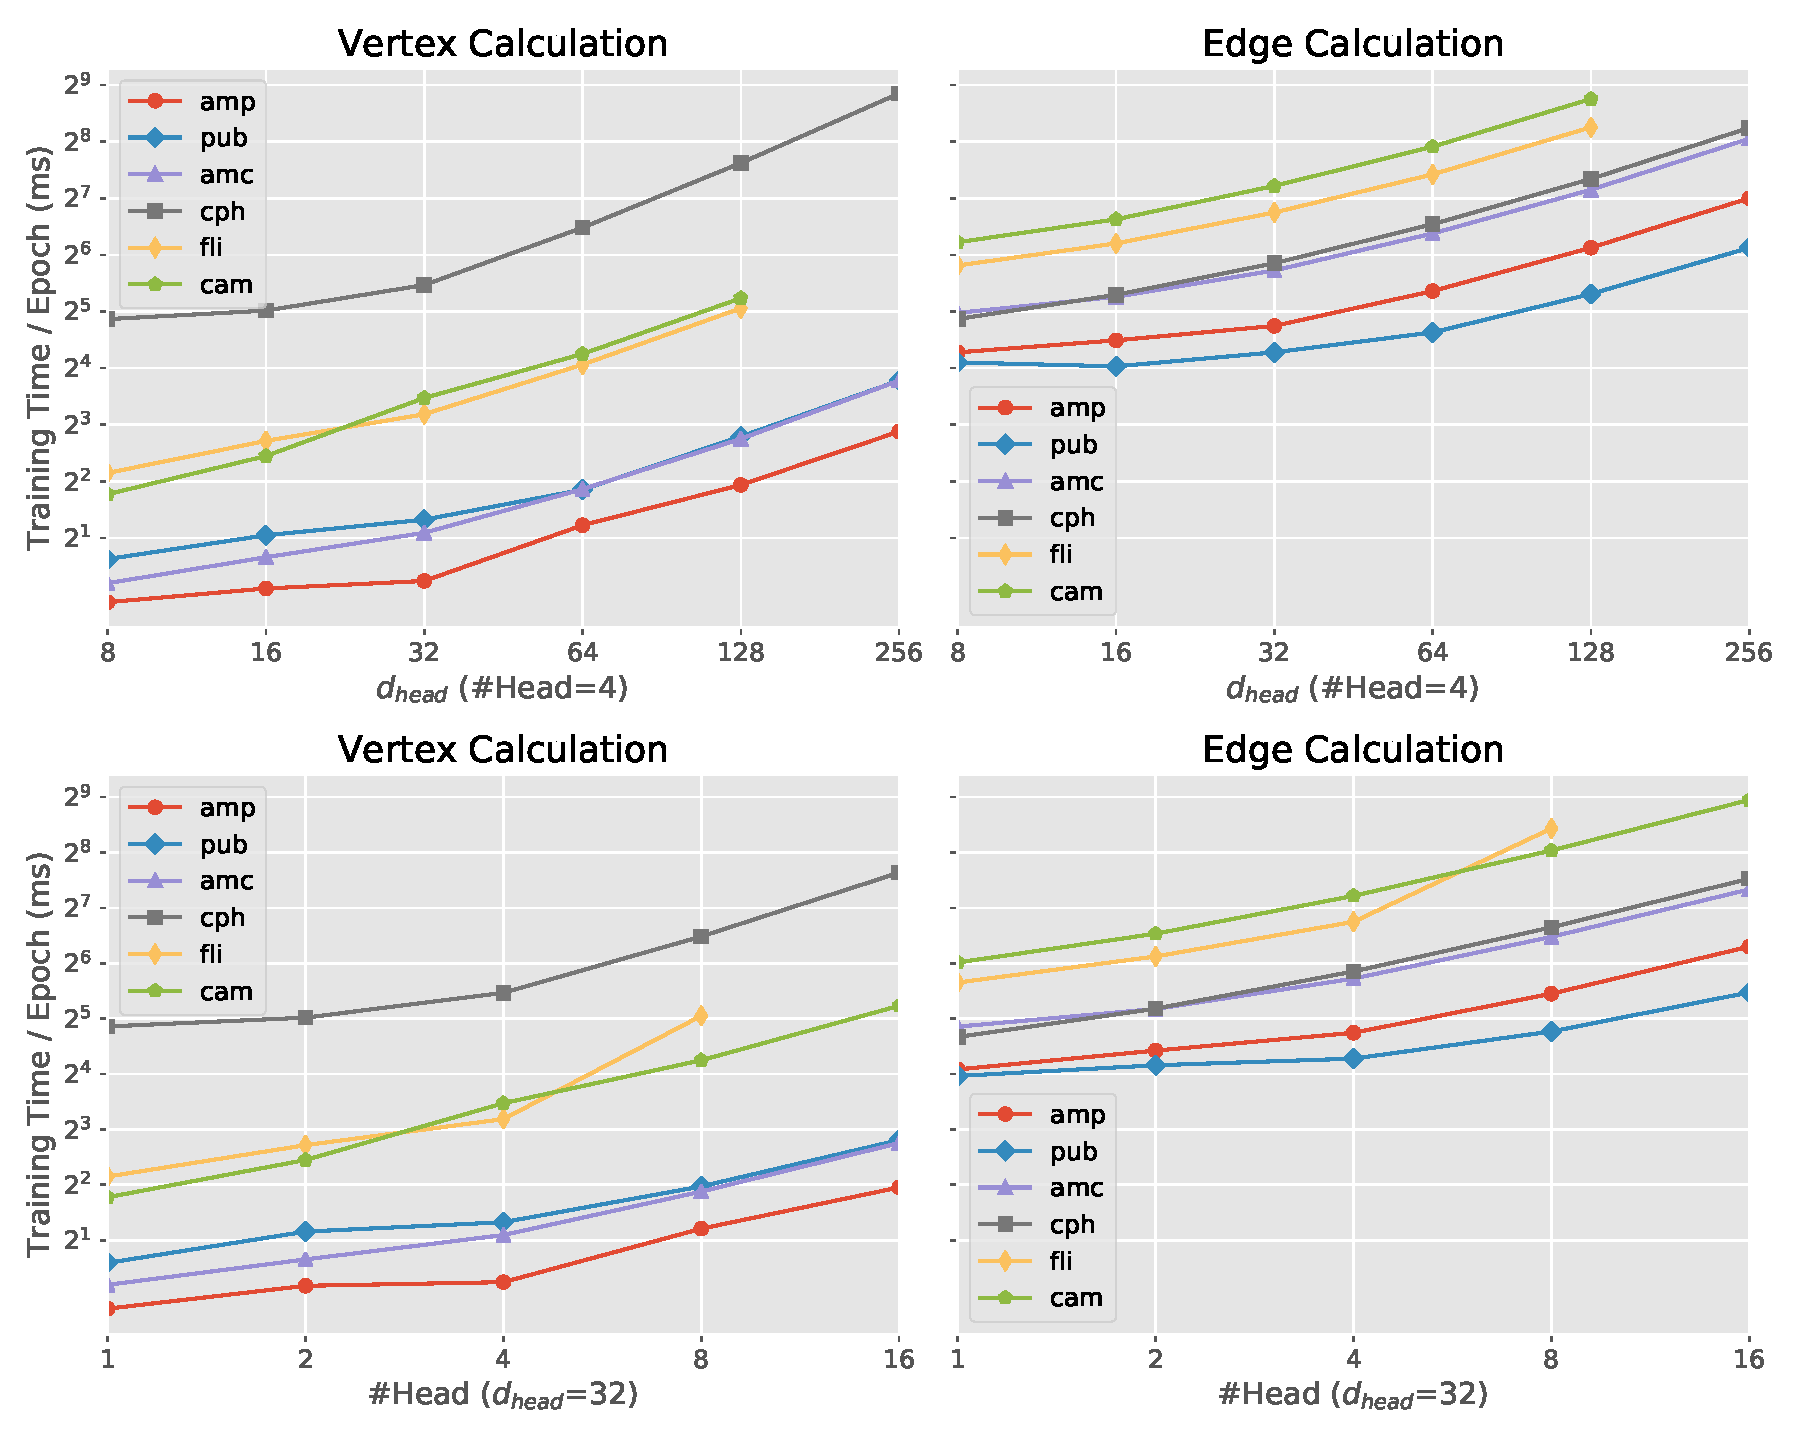
\includegraphics[width=0.6\textwidth]{figs/experiments/exp_hyperparameter_on_vertex_edge_phase_time_gat.pdf}
    \caption{Effects of hyper-parameters on the vertex/edge calculation time of GAT.}
    \label{fig:exp_hyperparameter_on_vertex_edge_phase_time_gat}
\end{figure}

\begin{figure}[H]
    \centering
    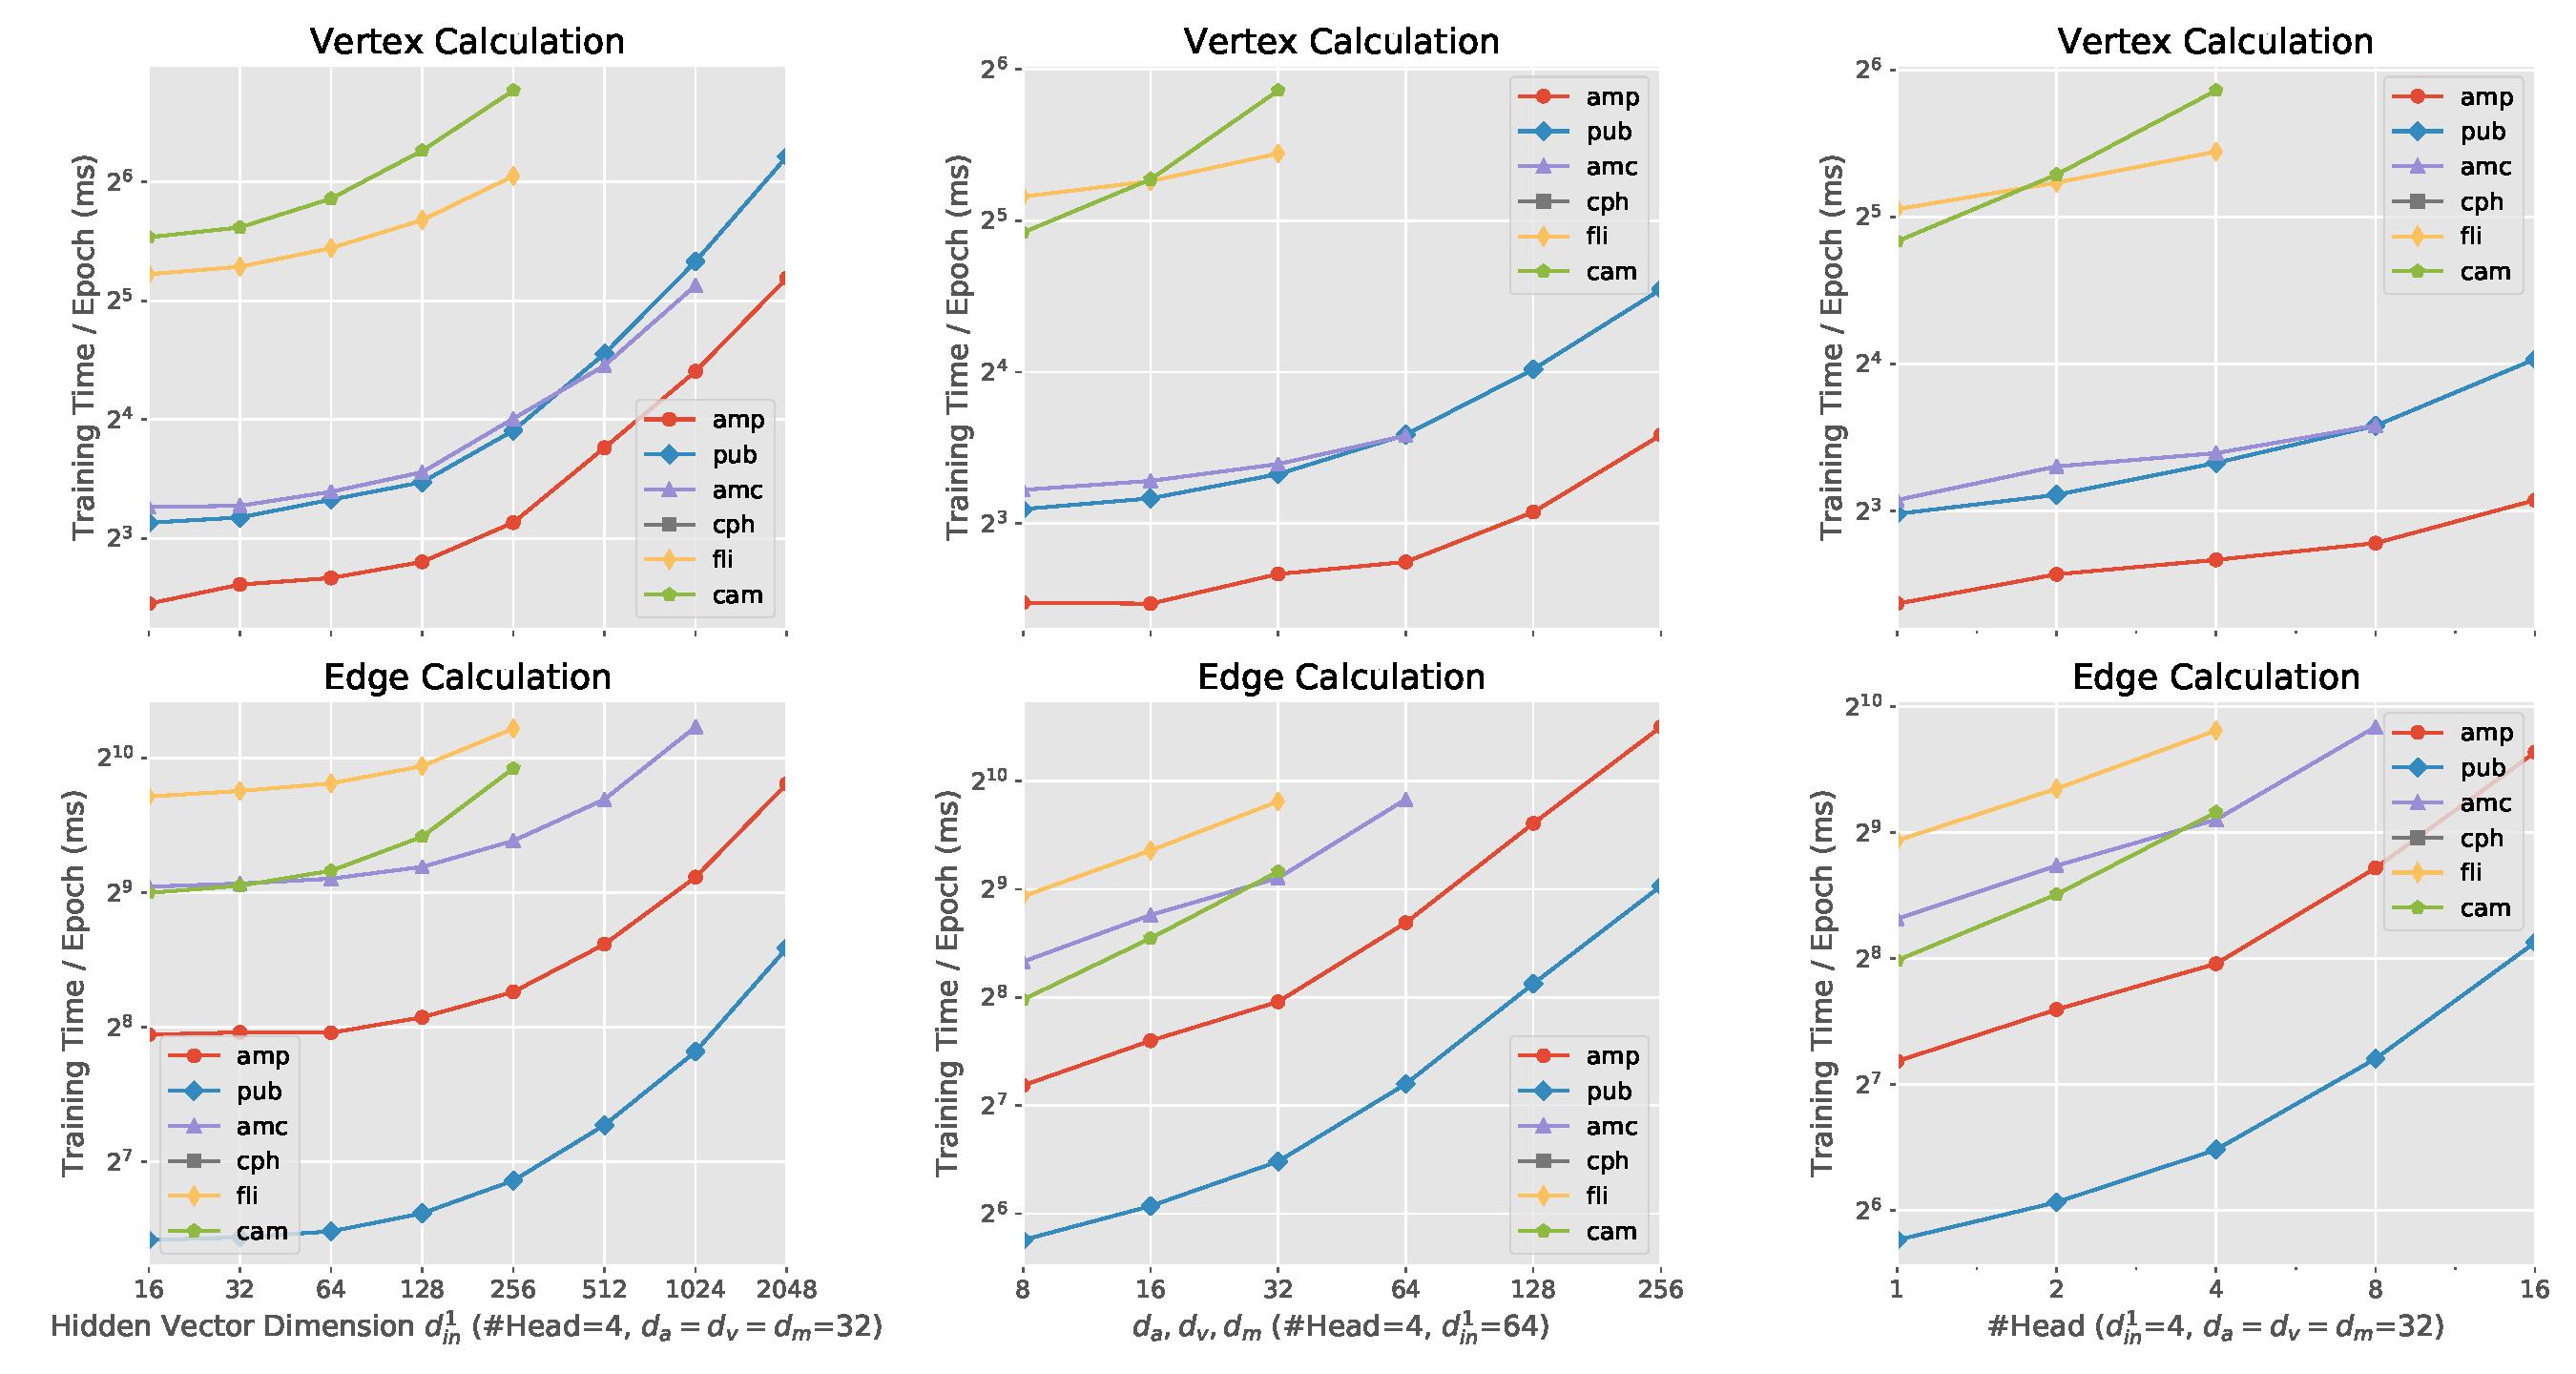
\includegraphics[width=0.8\textwidth]{figs/experiments/exp_hyperparameter_on_vertex_edge_phase_time_gaan.pdf}
    \caption{Effects of hyper-parameters on the vertex/edge calculation time of GaAN.}
    \label{fig:exp_hyperparameter_on_vertex_edge_phase_time_gaan}
\end{figure}

%\begin{figure}[H]
    %\centering
    %\subfloat[GCN\label{fig:exp_hyperparameter_on_vertex_edge_phase_time_gcn}]{\includegraphics[width=0.6\textwidth]%{figs/experiments/exp_hyperparameter_on_vertex_edge_phase_time_gcn.pdf}}
%    \\
    %\subfloat[GGNN\label{fig:exp_hyperparameter_on_vertex_edge_phase_time_ggnn}]{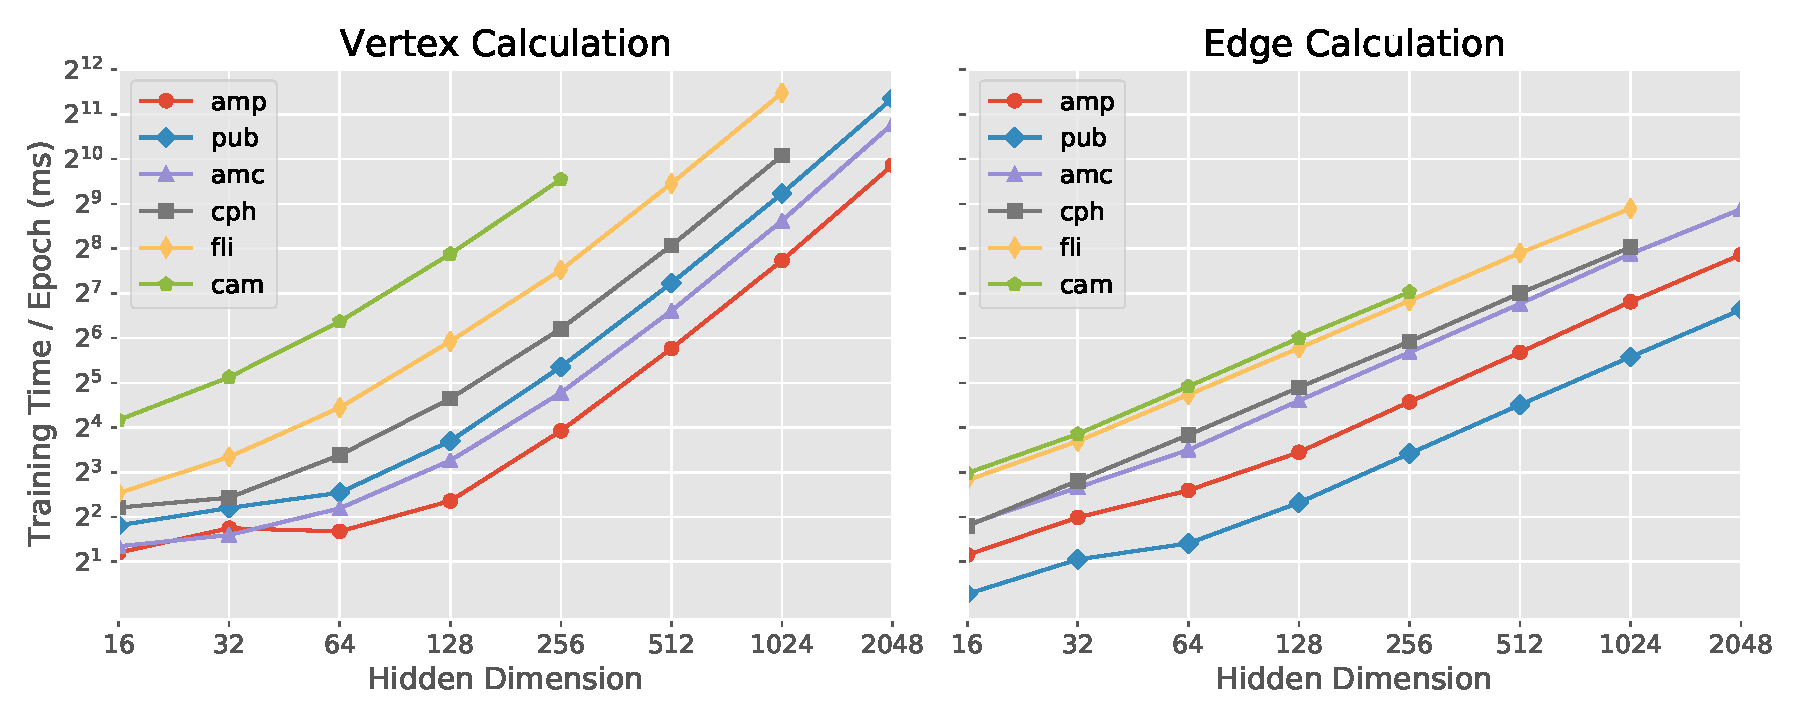
\includegraphics[width=0.6\textwidth]{figs/experiments/exp_hyperparameter_on_vertex_edge_phase_time_ggnn.pdf}}
%    \\
    %\subfloat[GAT\label{fig:exp_hyperparameter_on_vertex_edge_phase_time_gat}]{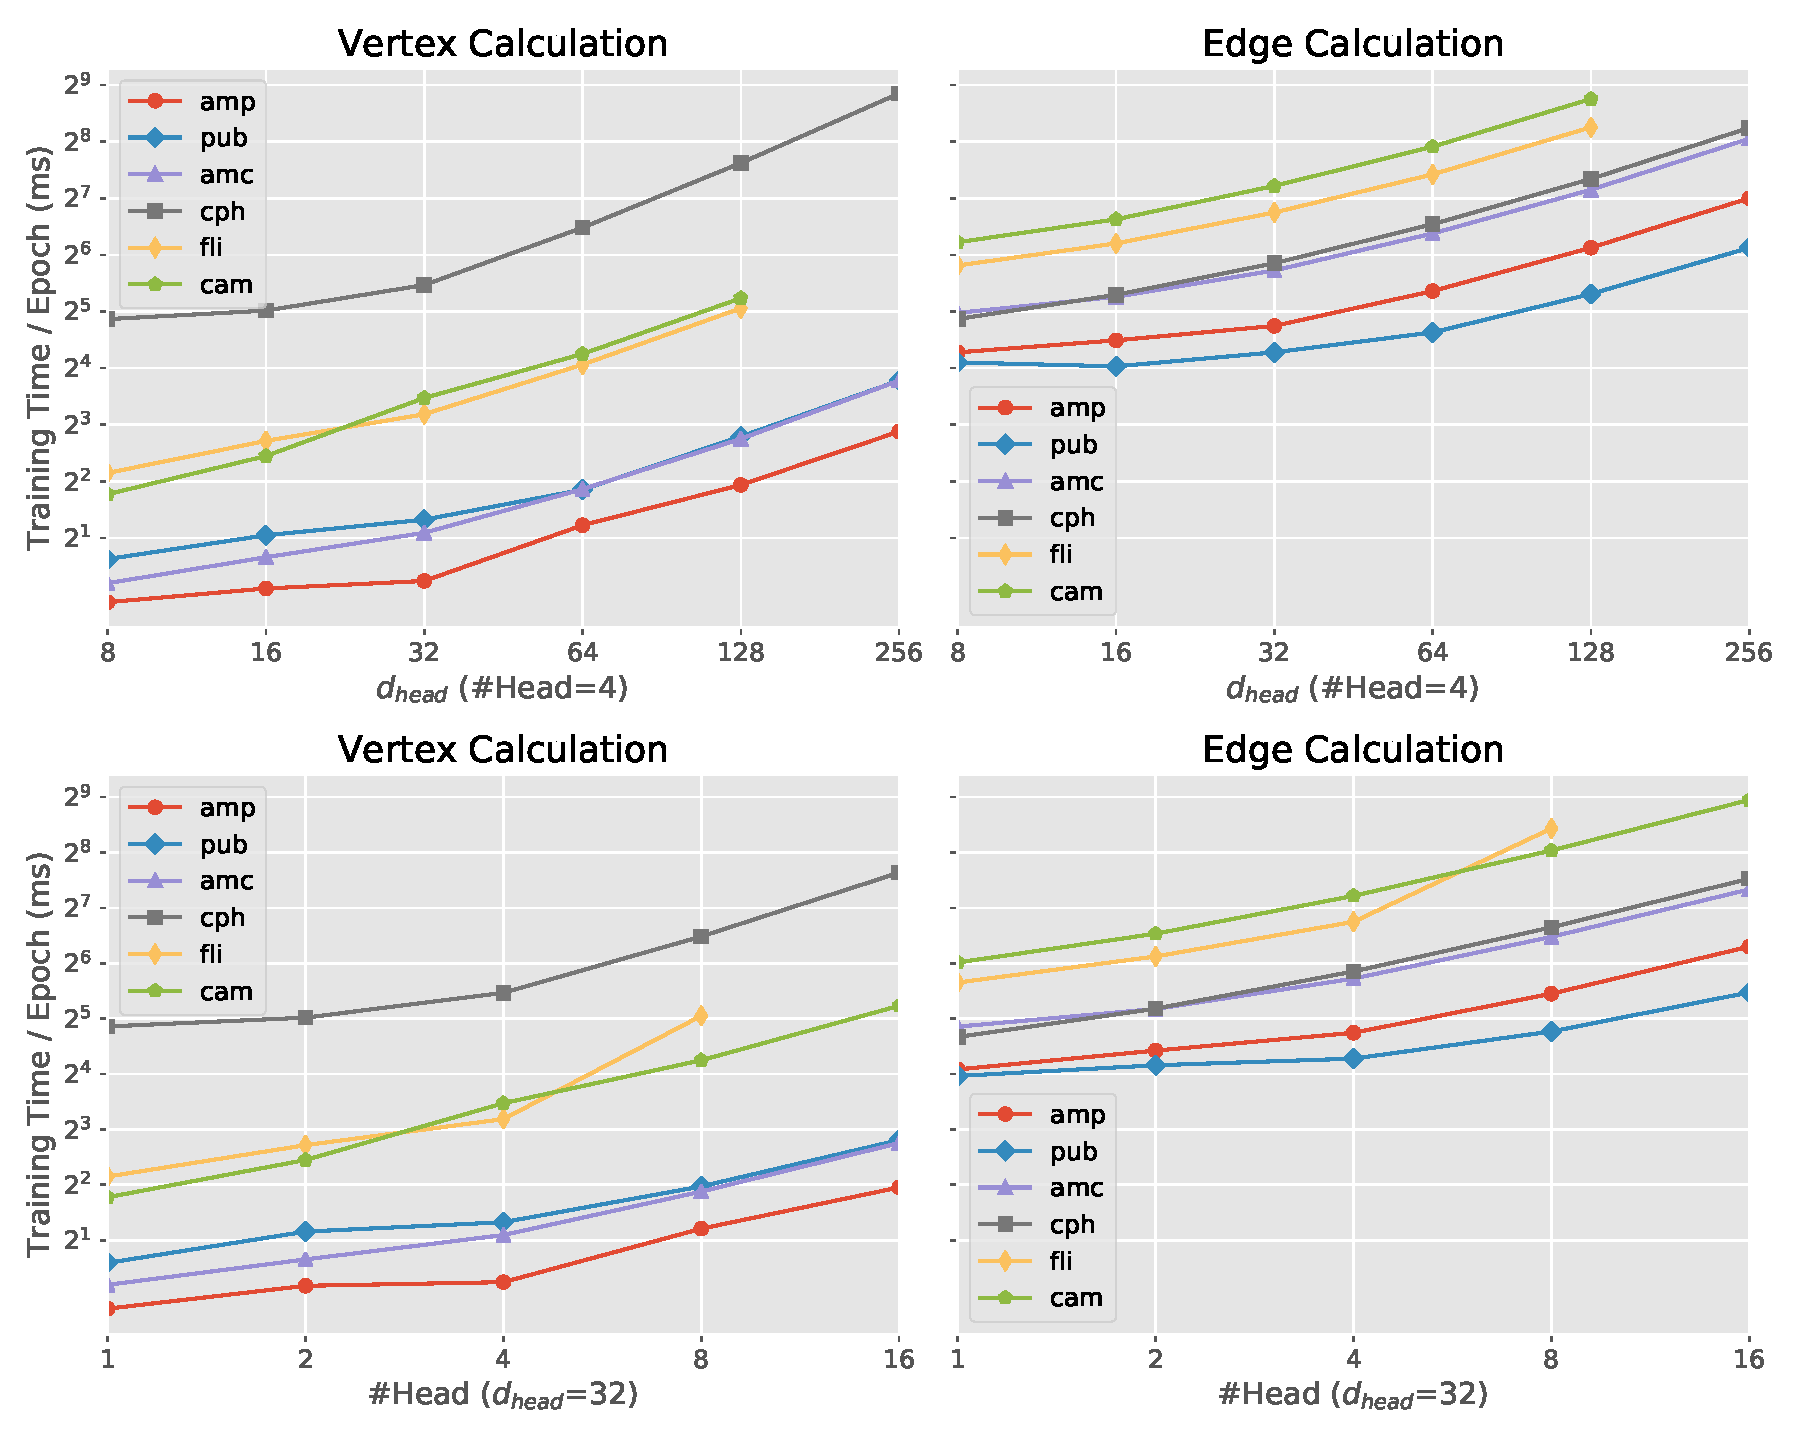
\includegraphics[width=0.6\textwidth]{figs/experiments/exp_hyperparameter_on_vertex_edge_phase_time_gat.pdf}}
    %\\
    %\subfloat[GaAN\label{fig:exp_hyperparameter_on_vertex_edge_phase_time_gaan}]{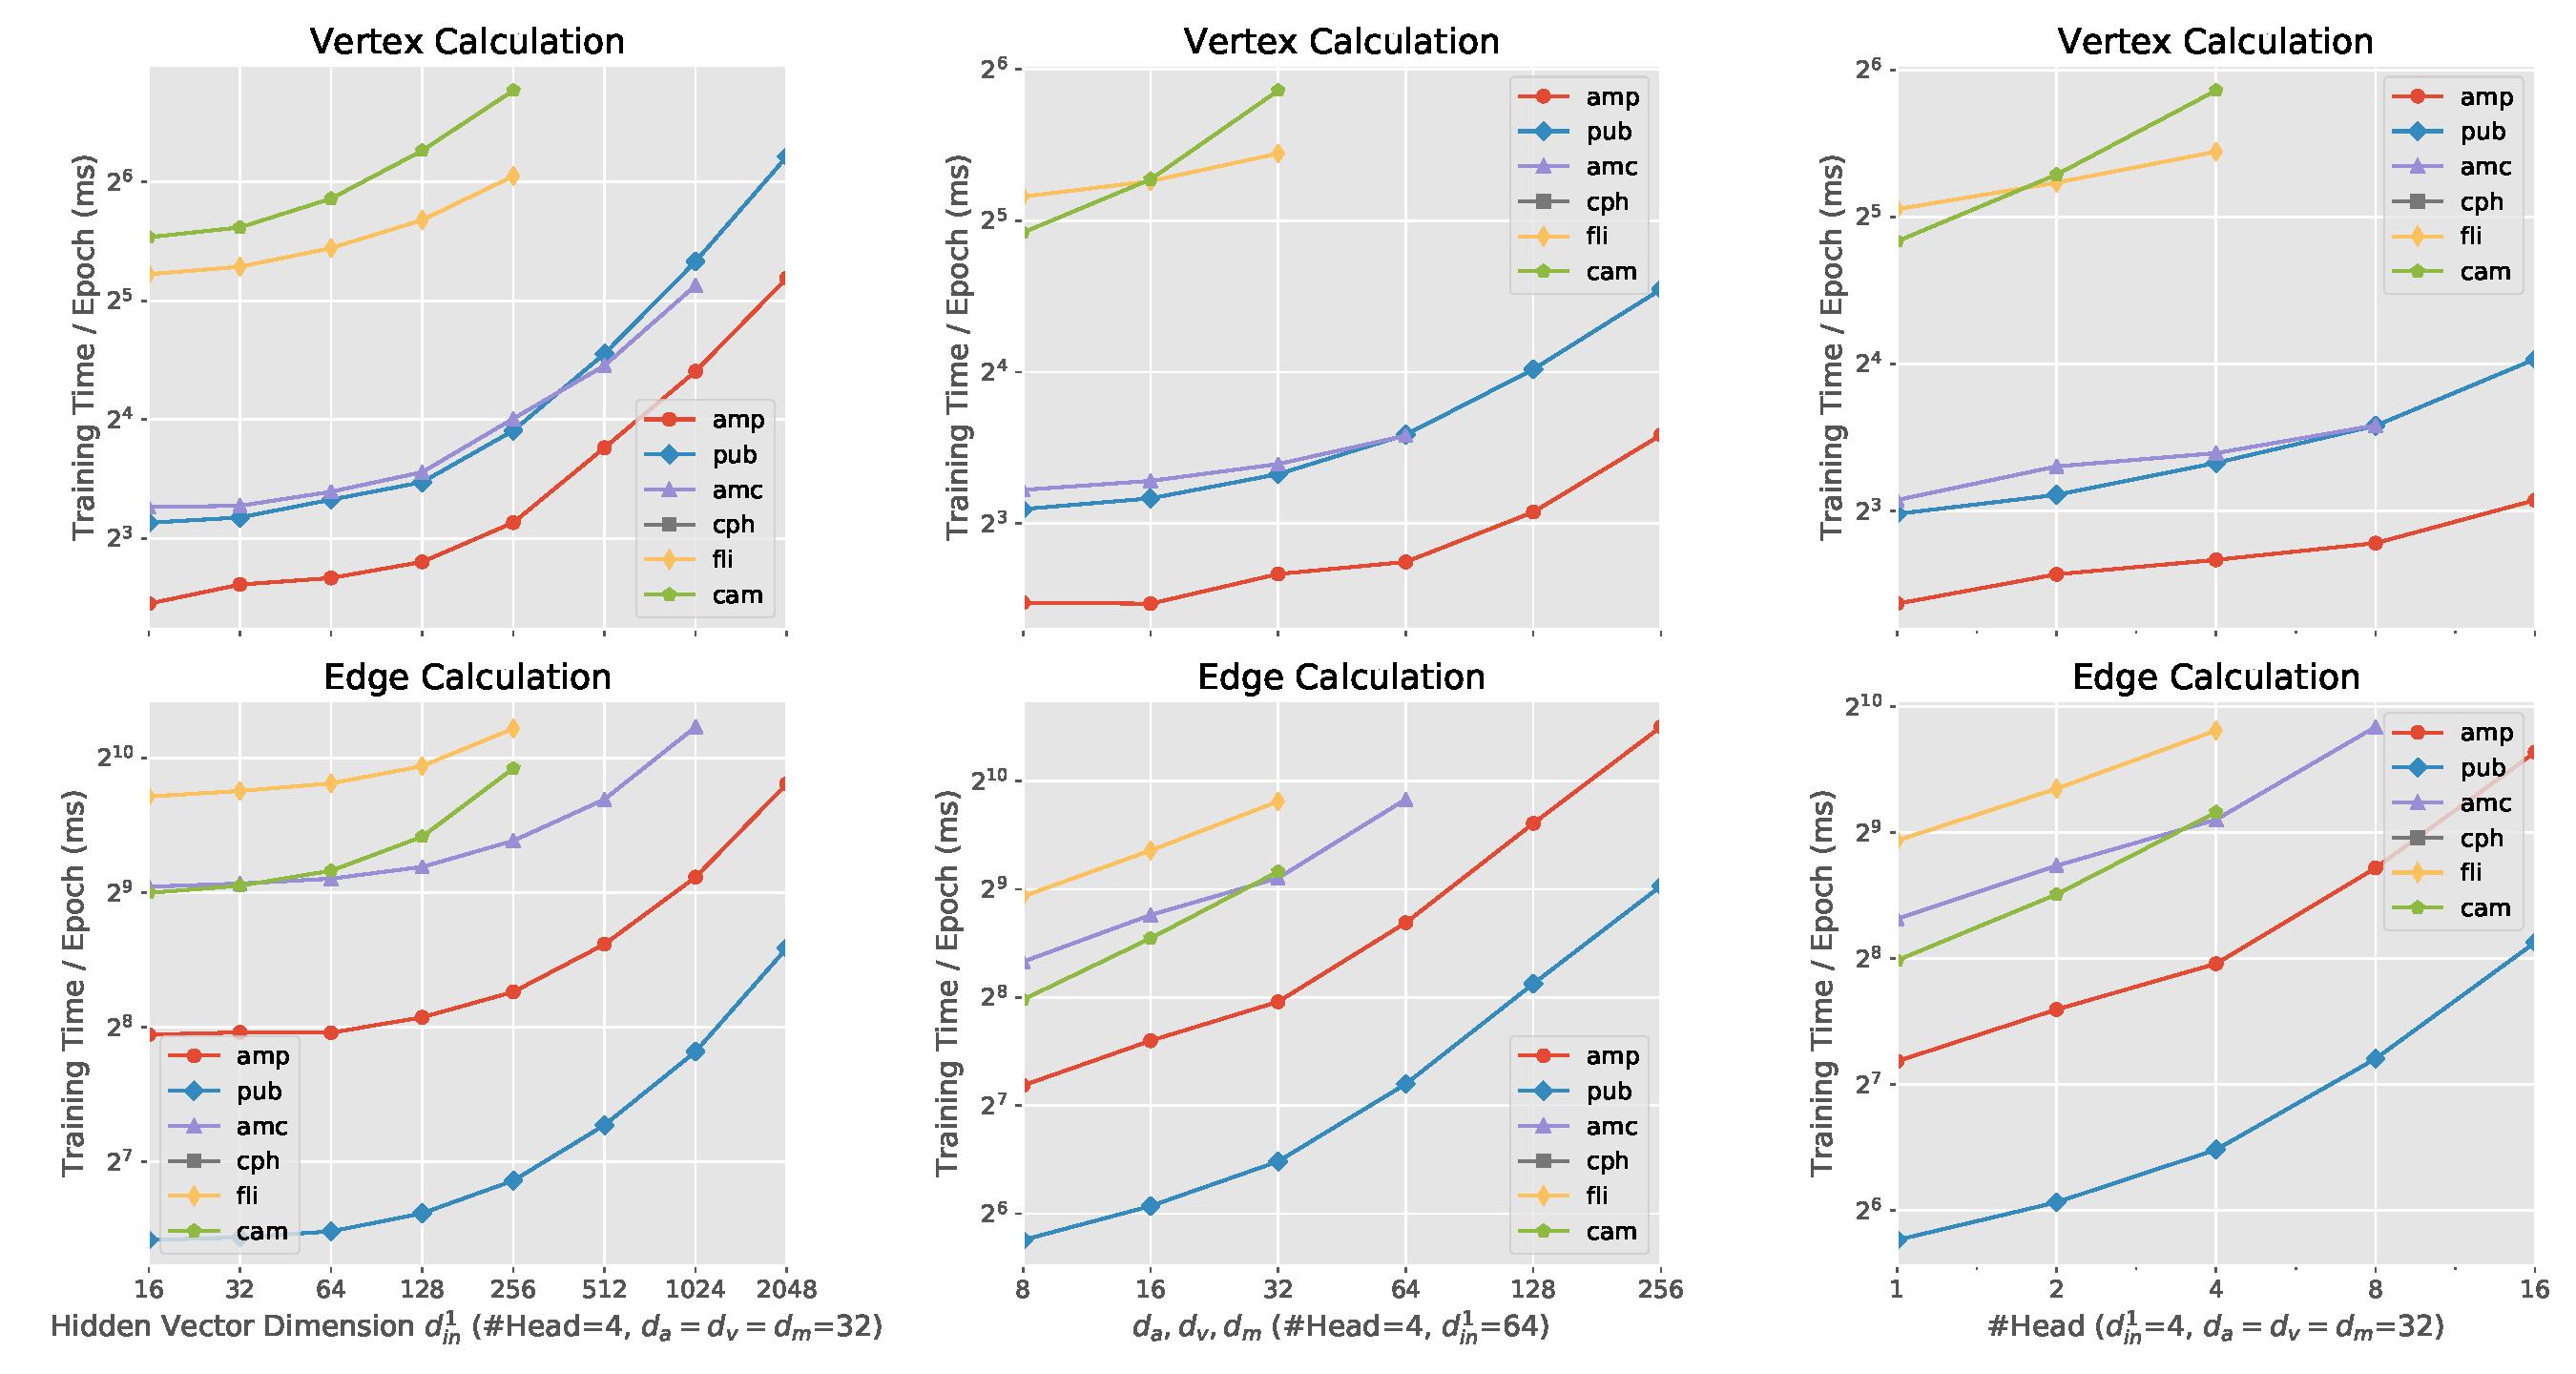
\includegraphics[width=0.9\textwidth]{figs/experiments/exp_hyperparameter_on_vertex_edge_phase_time_gaan.pdf}}

    %\caption{Effects of hyper-parameters on the edge/vertex calculation time.}
    %\label{fig:exp_hyperparameter_on_vertex_edge_phase_time}
%\end{figure}

For GCN and GGNN, $dim(\MyVec{h}^0_x)$ and $dim(\MyVec{h}^1_x)$ were solely determined by the dataset with $d^0_{in} = dim(\MyVec{h}^0_x) = dim(\MyVec{v_x})$ and $d^1_{out} = dim(\boldsymbol{h}^2_x)=\#Class$.
%
Therefore, the only modifiable hyper-parameter was the dimension of $\MyVec{h}^1_x$ that affected the dimension of output hidden vectors of the layer 0 $d^0_{out}$ and the dimension of input hidden vectors of the layer 1 $d^1_{in}$ simultaneously, i.e. $dim(\MyVec{h}^1_x)  = d^0_{out} = d^1_{in}$.
%
According to the time complexity analysis, if we fixed other hyper-parameters but only increased $dim(\boldsymbol{h}^1_x)$, the computational costs of the GNN layer 0 and the GNN layer 1 should both increase linearly with $dim(\boldsymbol{h}^1_x)$, causing the training time of the whole GNN also increasing linearly. 
%
\figurename~\ref{fig:exp_hyperparameter_on_vertex_edge_phase_time_gcn} and \figurename~\ref{fig:exp_hyperparameter_on_vertex_edge_phase_time_ggnn} show that the training time of GCN and GGNN increased linearly with $dim(\boldsymbol{h}^1_x)$ when $dim(\boldsymbol{h}^1_x)$ was big, consistent with the theoretical analysis.

For GAT, we modified the number of heads $K$ and the dimension of each head $d_{head}$ in the GAT layer 0.
%
The dimension of $\MyVec{h}^1_x$ is determined as $dim(\boldsymbol{h}^1_x) = K d_{head}$.
%
Thus, the computational costs of the GAT layer 0 and the GAT layer 1 should increase linearly with $K$ and $d_{head}$ separately. 
%
\figurename~\ref{fig:exp_hyperparameter_on_vertex_edge_phase_time_gat} confirms the theoretical analysis.

For GaAN, it is also based on the multi-head mechanism.
%
Its time complexity should be affected by $dim(\boldsymbol{h}^1_x)$ ($d^0_{out} = d^1_{in} = dim(\boldsymbol{h}^1_x)$), $d_a$, $d_v$, $d_m$, and the number of heads $K$.
%
\figurename~\ref{fig:exp_hyperparameter_on_vertex_edge_phase_time_gaan} demonstrates that the training time increased linearly with the hyper-parameters, except for $dim(\boldsymbol{h}^1_x)$.
As $dim(\boldsymbol{h}^1_x)$ increased, the training time increased first slightly and then linearly.
We observed similar phenomena in GCN, GGNN, and GAT:
When the values of hyper-parameters were too low, GNN training could not make full use of the computing power of the GPU.
%
When the values of hyper-parameters became high enough, training time increased linearly, supporting the time complexity analysis.

\paragraph{Effects on Peak Memory Usage}

We further measured the effects of the hyper-parameters on the peak GPU memory usage during training in \figurename~\ref{fig:exp_hyperparameter_memory_usage}.
%
The memory usage also increased linearly as the hyper-parameters increased for all GNNs, except for GaAN on $dim(\MyVec{h}^1_x)$.
%
As the hidden vectors $\MyVec{h}^1_x$ consumed a small proportion of memory in GaAN, the growth in the memory usage was not noticeable until $dim(\boldsymbol{h}^1_x)$ was large enough.

\begin{figure}[H]
    \centering
    \subfloat[GCN]{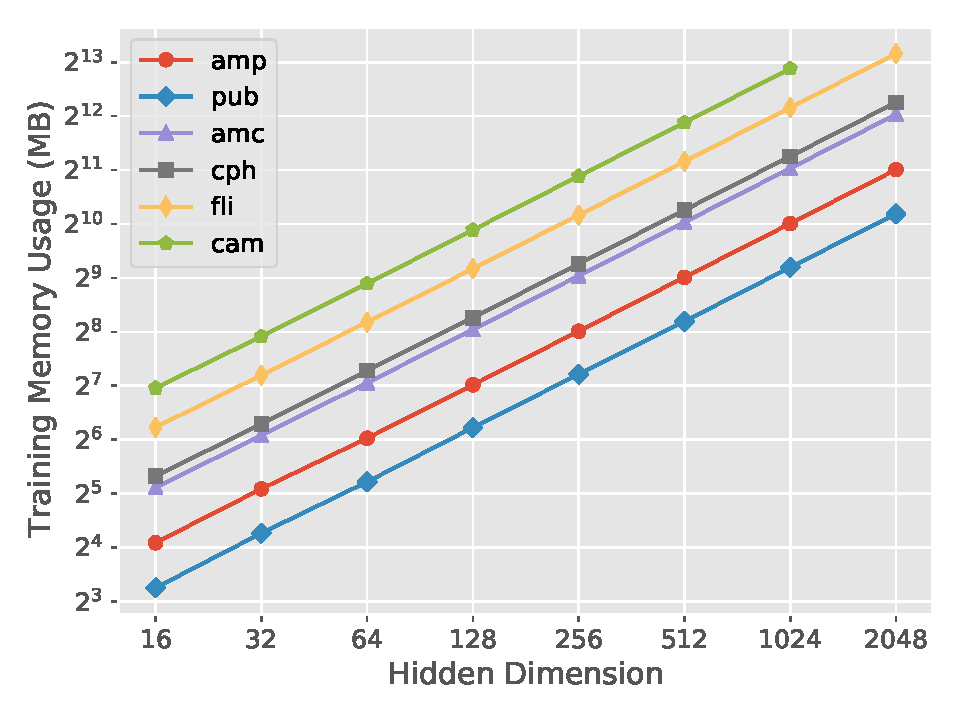
\includegraphics[width=0.25\columnwidth]{figs/experiments/exp_hyperparameter_on_memory_usage_gcn.pdf}}
    \subfloat[GGNN]{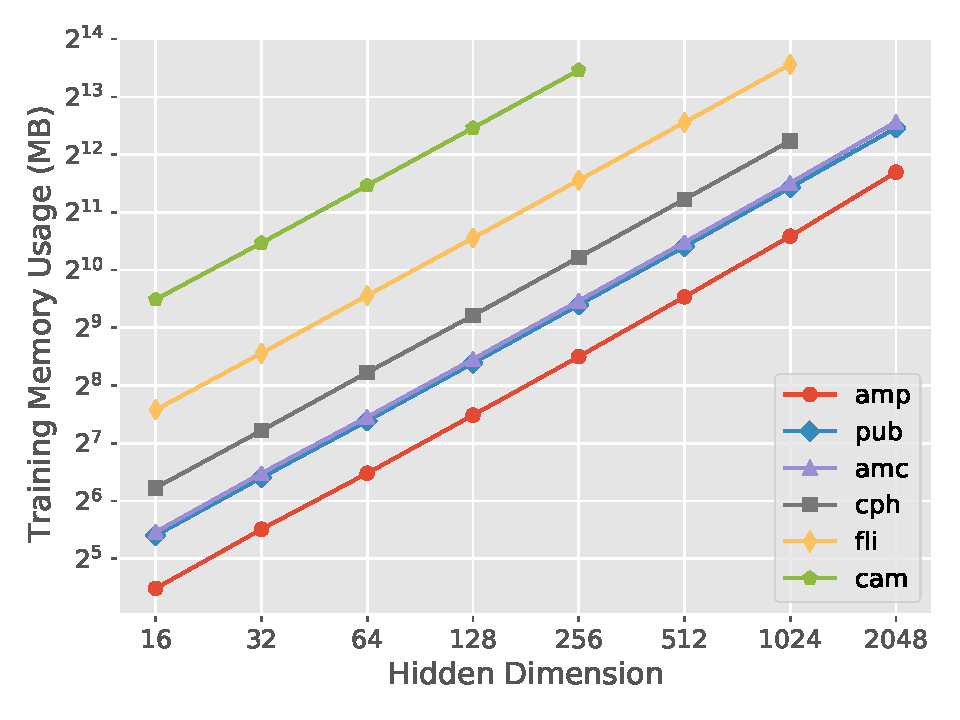
\includegraphics[width=0.25\columnwidth]{figs/experiments/exp_hyperparameter_on_memory_usage_ggnn.pdf}}\\
    \subfloat[GAT]{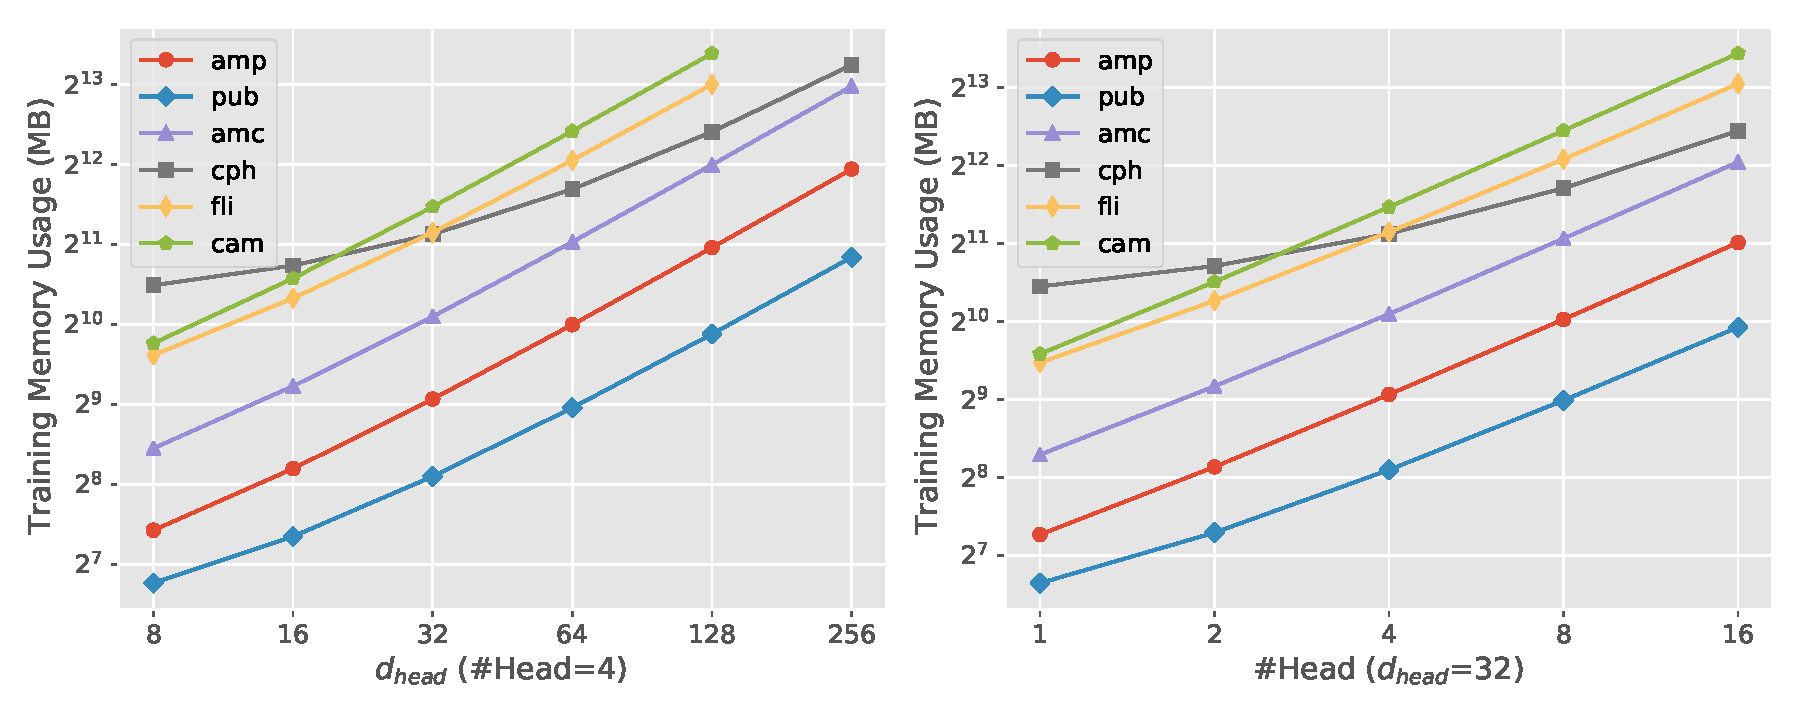
\includegraphics[width=0.5\columnwidth]{figs/experiments/exp_hyperparameter_on_memory_usage_gat.pdf}}\\
    \subfloat[GaAN]{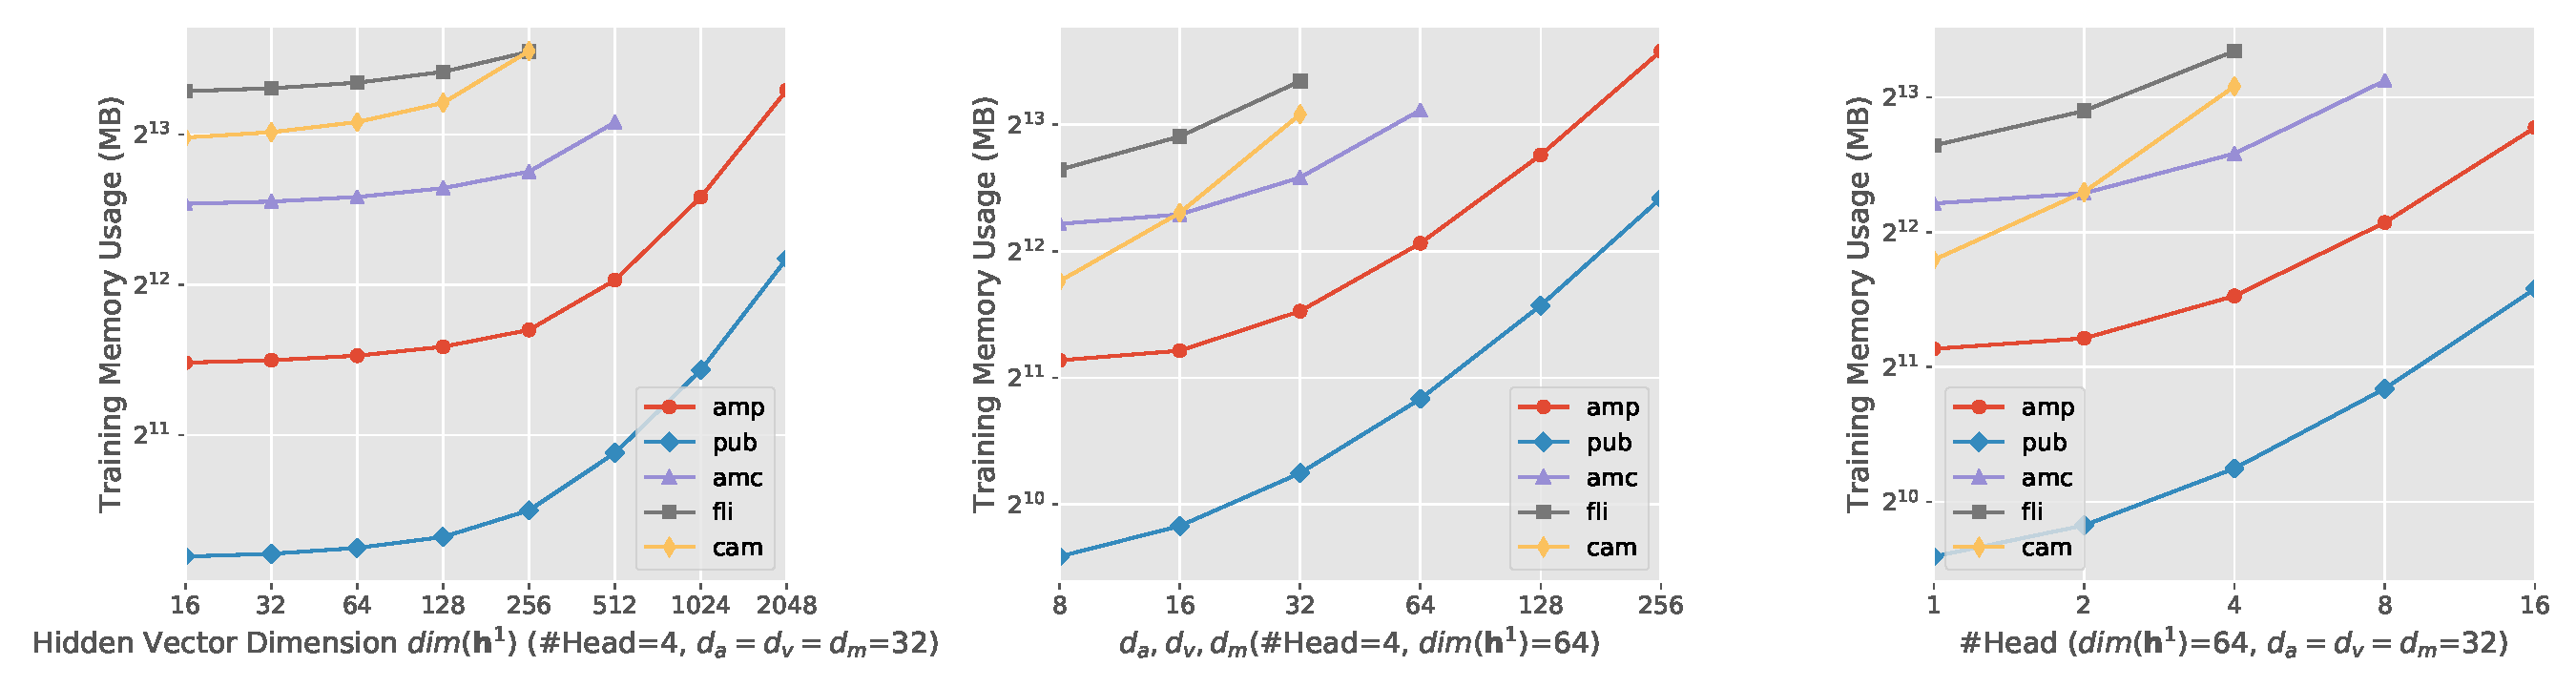
\includegraphics[width=0.75\columnwidth]{figs/experiments/exp_hyperparameter_on_memory_usage_gaan.pdf}}
    \caption{Effects of hyper-parameters on the peak GPU memory usage during training, excluding the memory used by the dataset and the model parameters.}
    \label{fig:exp_hyperparameter_memory_usage}
\end{figure}

\paragraph{Effects on Accuracy}

The relationship between hyper-parameters of GNNs (i.e., model complexity) and accuracy is very complicated, and there is no clear theoretical analysis yet.
%
Generally speaking, higher model complexity can bring stronger expressive ability and may bring higher accuracy, but it also increases the risk of overfitting.
%
To evaluate the effects of hyper-parameters on accuracy, we measured the accuracy of the four typical GNNs under different hyper-parameters.
%
\figurename~\ref{fig:exp_hyperparameter_accuracy} shows the experimental results.

For GCN, the accuracy was sensitive to the dimension of hidden vectors $dim(\MyVec{h}^1_x)$.
%
As $dim(\MyVec{h}^1_x)$ increased, the accuracy first increased quickly and then stabilized when $dim(\MyVec{h}_x^1) \geq 8$.
%
For GGNN, its accuracy curves showed similar trends as GCN.
%
However, GGNN was more sensitive to $dim(\MyVec{h}_x^1)$ than GCN and the accuracy even decreased when $dim(\MyVec{h}_x^1) \geq 1024$.
%
Since GGNN had high model complexity (with 13 weight matrices/vectors to train), GGNN might occur overfitting in those cases.
%%%% TODO %%%%


%In deep learning, accuracy is also an important indicator that algorithm engineers care about.
%
%We adopted a unified standard (section \ref{sec:hyper-parameters}) to evaluate the effect of hyper-parameters on accuracy.
%
%\figurename~\ref{fig:exp_hyperparameter_accuracy} shows how the accuracy varies with hyper-parameters.
%
%For all models, we found that different datasets had different curve changes, that was, different datasets had different sensitivity to hyper-parameter changes.
%
%This was because different datasets had different characteristics, which lead to different learning difficulties.
%

Except for the effect of the number of heads on GAT and the effect of $d_a$, $d_v$, $d_m$, the number of heads $K$ on GaAN, we found the same phenomena:
the accuracy of the model was often low when hyper-parameters were low. When a certain threshold was reached, the accuracy began to fall within the range of fluctuations.
%
We conducted additional experiments for these exceptions. Taking the effect of the number of heads on GAT as an example, 
\figurename~\ref{fig:exp_hyperparameter_accuracy_gat_small_info} shows the trend is similar to the phenomena discussed above when $d_{head}$ is adjusted to a smaller value such as 2 and 4.
%
This phenomenon showed some relationship between accuracy and model complexity.
%
When the hyper-parameter value was very small, the model complexity was often low, which limited the expressive ability of the model.
%
In this case, accuracy and model complexity were positively related.
%
However, when the hyper-parameter increased to a certain threshold, the model had sufficient learning ability, and the relationship between accuracy and model complexity was no longer certain.
% added by wangyupan, 2020-12-22 ----end----

\begin{figure}[H]
    \centering
    \subfloat[GCN]{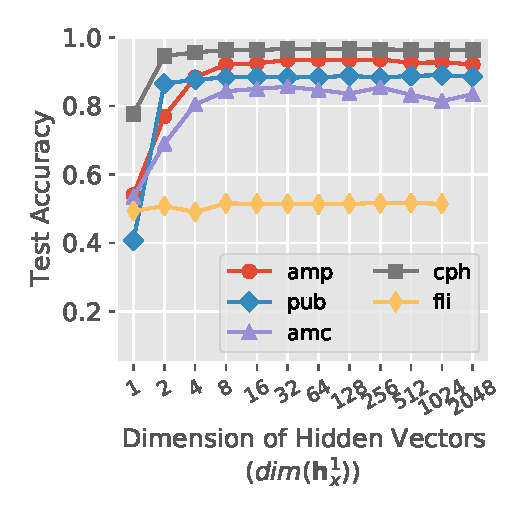
\includegraphics[width=0.3\columnwidth]{figs/experiments/exp_hyperparameter_on_accuracy_gcn.pdf}}
    \subfloat[GGNN]{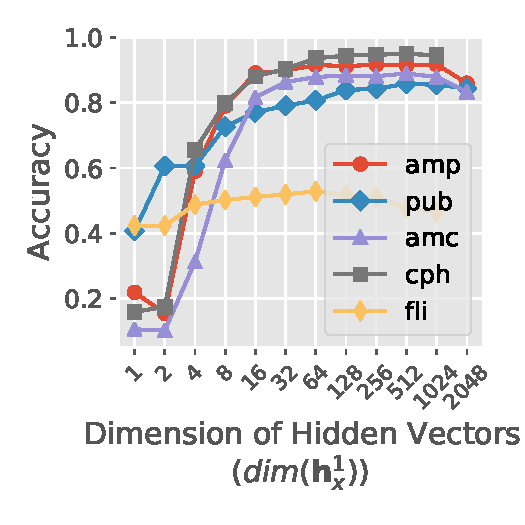
\includegraphics[width=0.3\columnwidth]{figs/experiments/exp_hyperparameter_on_accuracy_ggnn.pdf}}\\
    \subfloat[GAT]{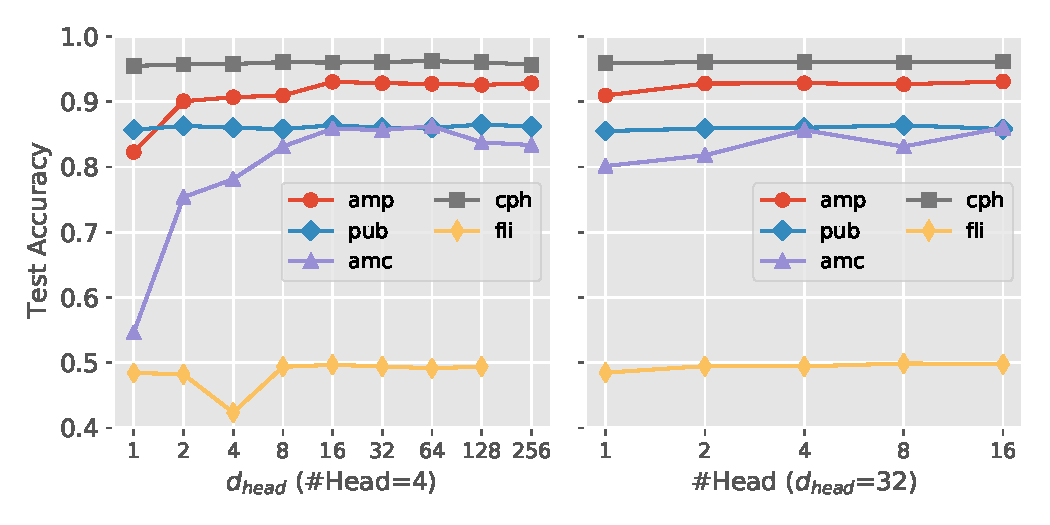
\includegraphics[width=0.6\columnwidth]{figs/experiments/exp_hyperparameter_on_accuracy_gat.pdf}}\\
    \subfloat[GaAN]{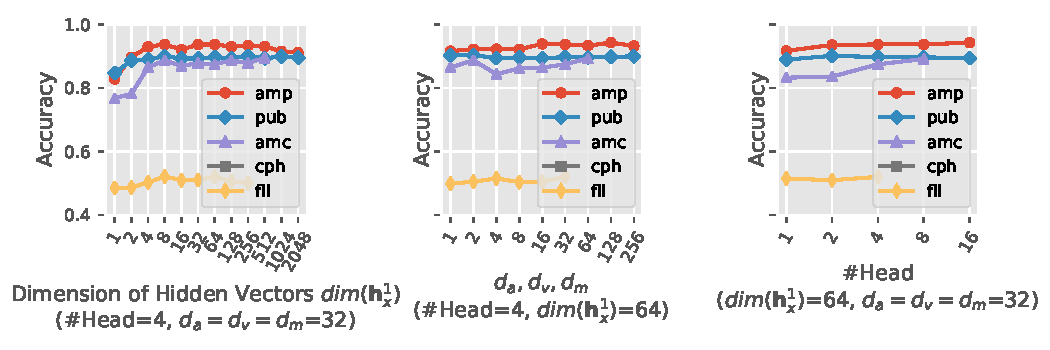
\includegraphics[width=0.85\columnwidth]{figs/experiments/exp_hyperparameter_on_accuracy_gaan.pdf}}
    \caption{Effects of hyper-parameters on accuracy of the typical GNNs.}
    \label{fig:exp_hyperparameter_accuracy}
\end{figure}

\begin{figure}[H]
    \centering
    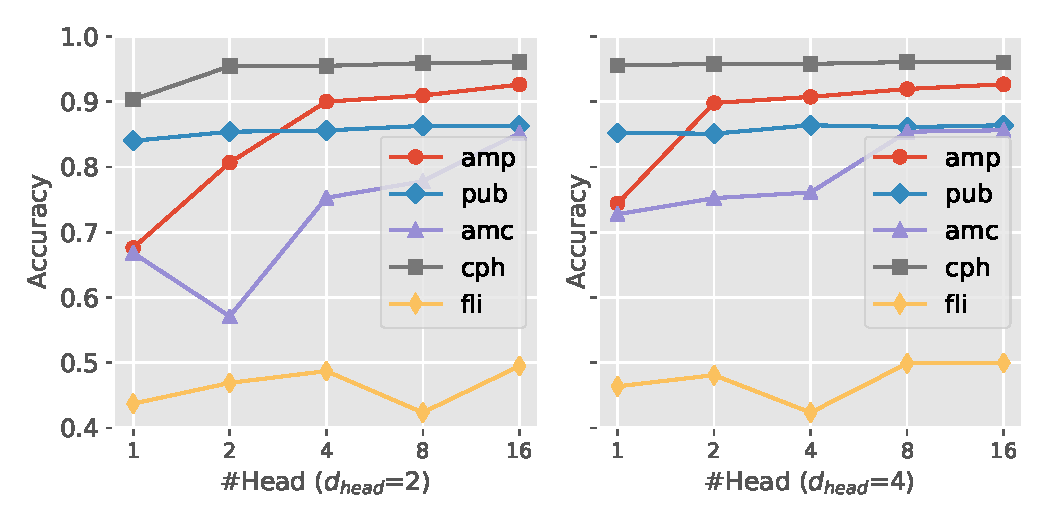
\includegraphics[width=0.5\columnwidth]{figs/experiments/exp_hyperparameter_on_accuracy_gat_small_info.pdf}
    \caption{Effects of the number of heads on GAT ($d_{head}$=2,4)}
    \label{fig:exp_hyperparameter_accuracy_gat_small_info}
\end{figure}

\paragraph{Summary}

The complexity analysis in \tablename~\ref{tab:gnn_overview_edge} and \tablename~\ref{tab:gnn_overview_vertex} was valid.
%
Fixing other hyper-parameters, each hyper-parameter itself affected the training time and the memory usage of a GNN Layer \emph{in a linear way}.
%
Algorithm engineers could adjust hyper-parameters according to the time complexity to avoid explosive growth in the training time and memory usage.
%
% added by wangyupan, 2020-12-22 ----start----
There was no definite relationship between accuracy and hyper-parameters. 
%
To obtain the optimal model, hyper-parameters needed to be manually adjusted by algorithm engineers.
% added by wangyupan, 2020-12-22 ----end----

\subsection{Training Time Breakdown}
\label{sec:training_time_breakdown}

To find out which stage/step dominated the training time, we decomposed the training time and analyzed performance bottlenecks level by level.

\subsubsection{Layer Level}

\figurename~\ref{fig:exp_vertex_edge_cal_proportion} decomposes the training time of a GNN on the layer level.
%
The training time of each layer was the summation of the time in the forward, backward, and evaluation phases.
%
In GCN, GAT, and GaAN, the time spent on the layer 0 was much larger than the layer 1.
%
In those GNNs, the dimensions of the input/output hidden vectors in the layer 0 were much larger than the dimensions in the layer 1: $d^0_{in}=dim(\boldsymbol{v}_x)$, $d^0_{out}=d^1_{in}=64$, $d^1_{out}=\#Class$, and $dim(\boldsymbol{v}_x) \gg \#Class$.
%
For GaAN, since it required the dimensions of the input/output hidden vectors must be the same, the hyper-parameters were set to $d^0_{in}=d^0_{out}=d^1_{in}=d^1_{out}=64$ and the training time of both layers was close.

\begin{figure}[H]
    \centering
    \subfloat[GCN]{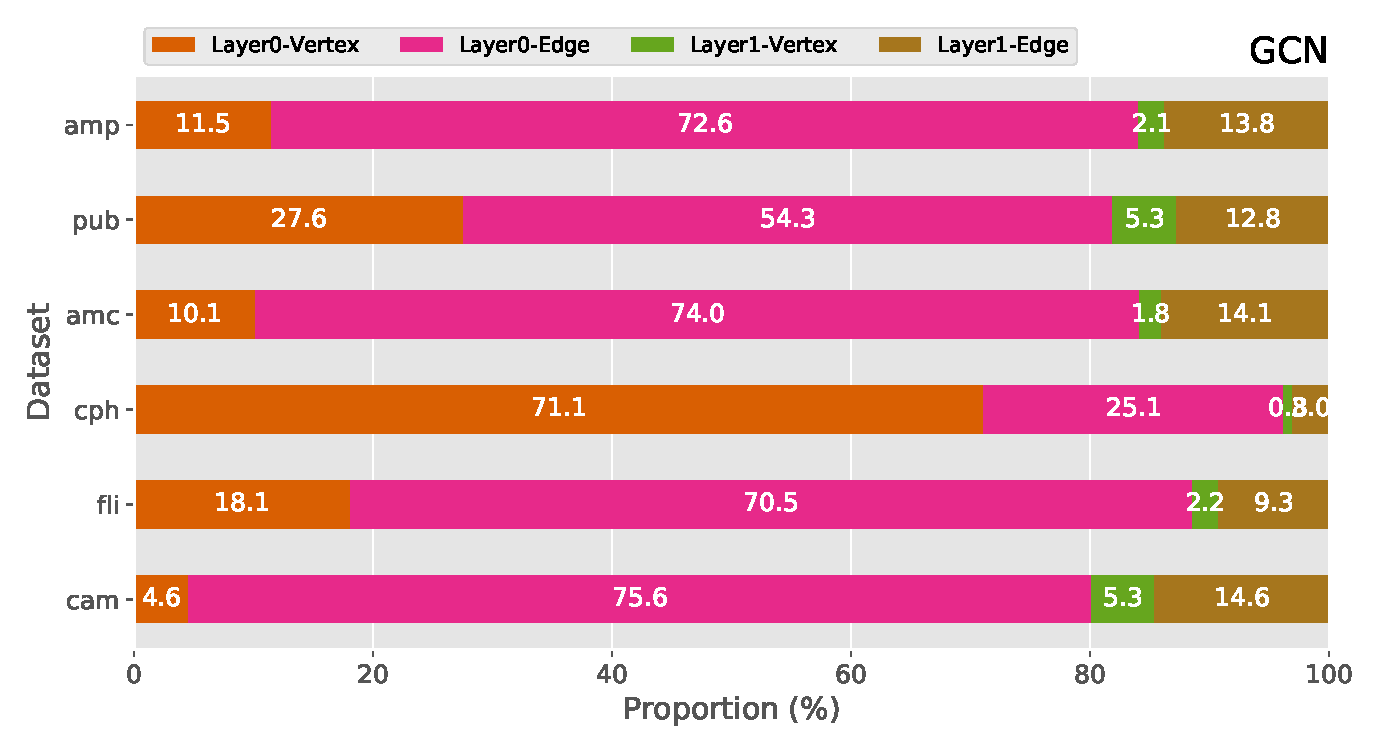
\includegraphics[height=4.6cm]{figs/experiments/exp_layer_time_proportion_gcn.pdf}}
    \subfloat[GGNN]{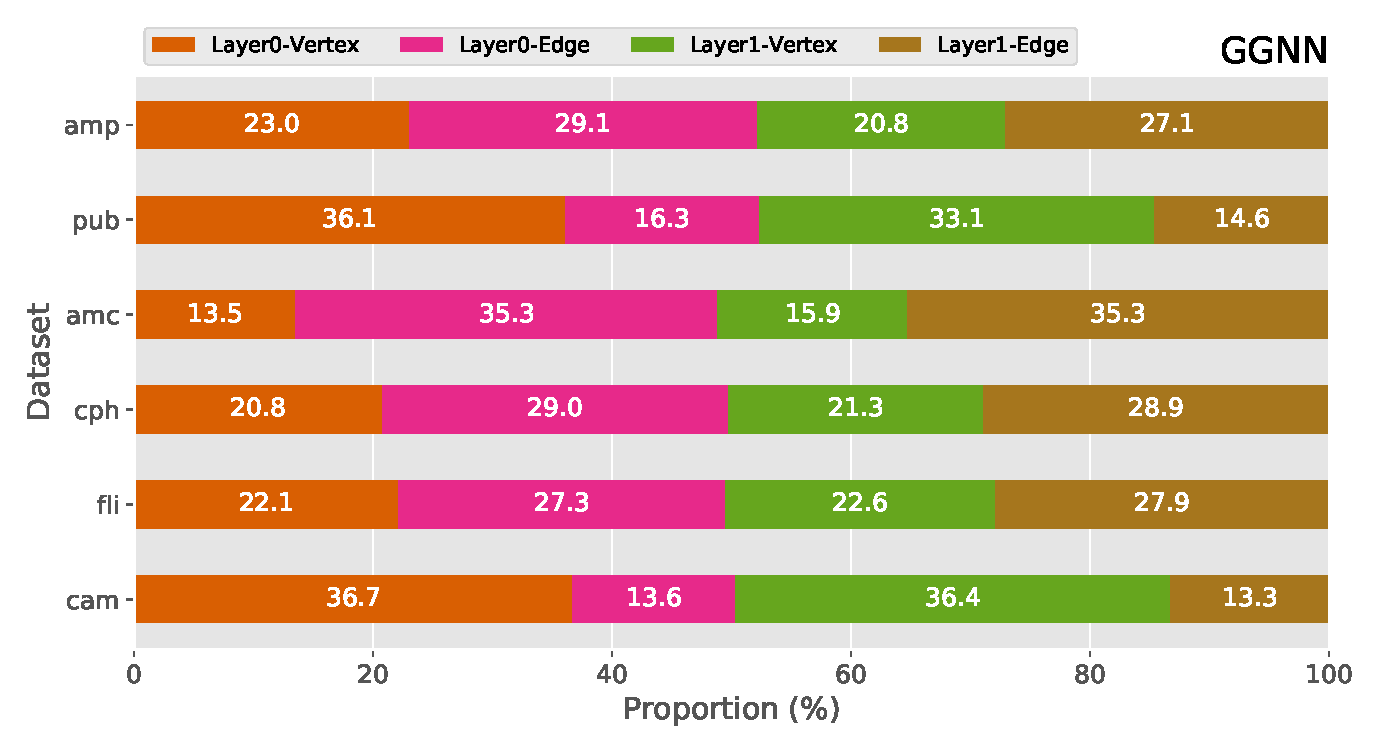
\includegraphics[height=4.6cm]{figs/experiments/exp_layer_time_proportion_ggnn.pdf}}\\
    \subfloat[GAT]{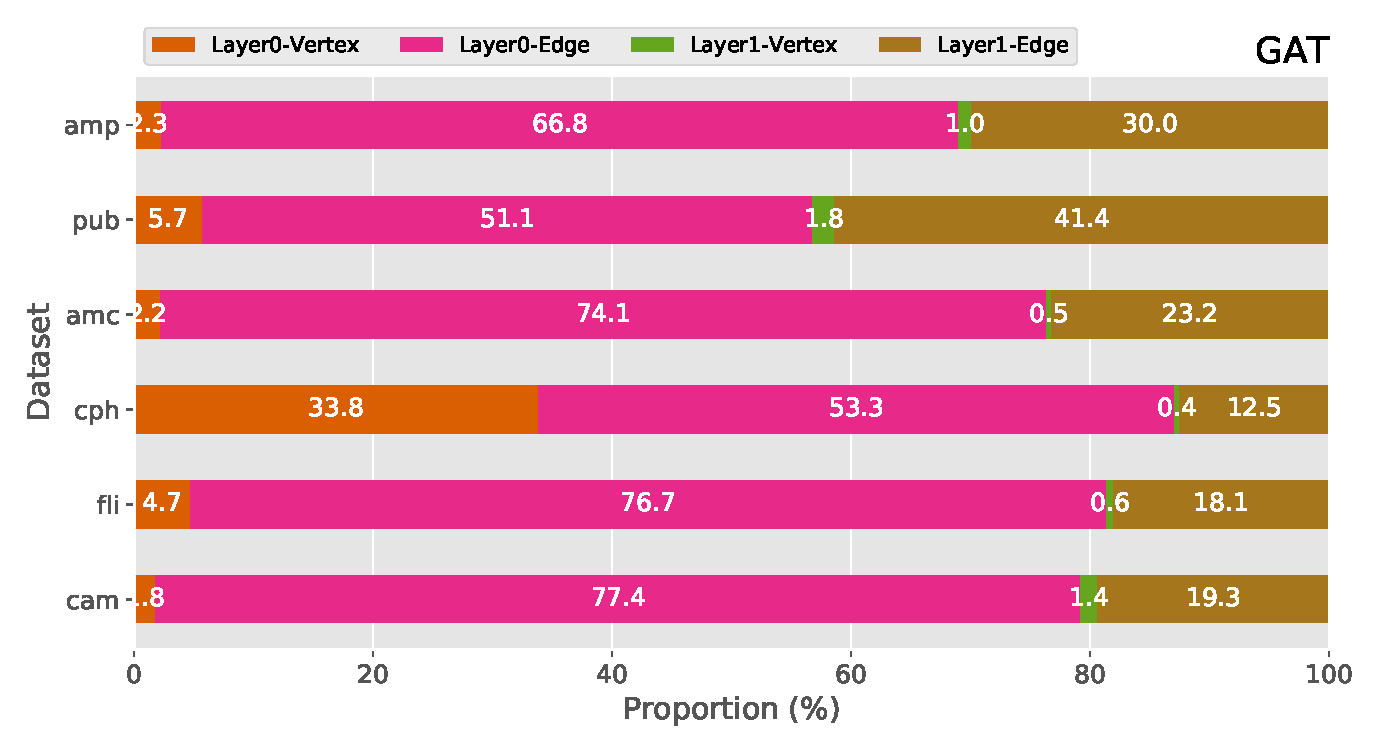
\includegraphics[height=4.6cm]{figs/experiments/exp_layer_time_proportion_gat.pdf}}
    \subfloat[GaAN]{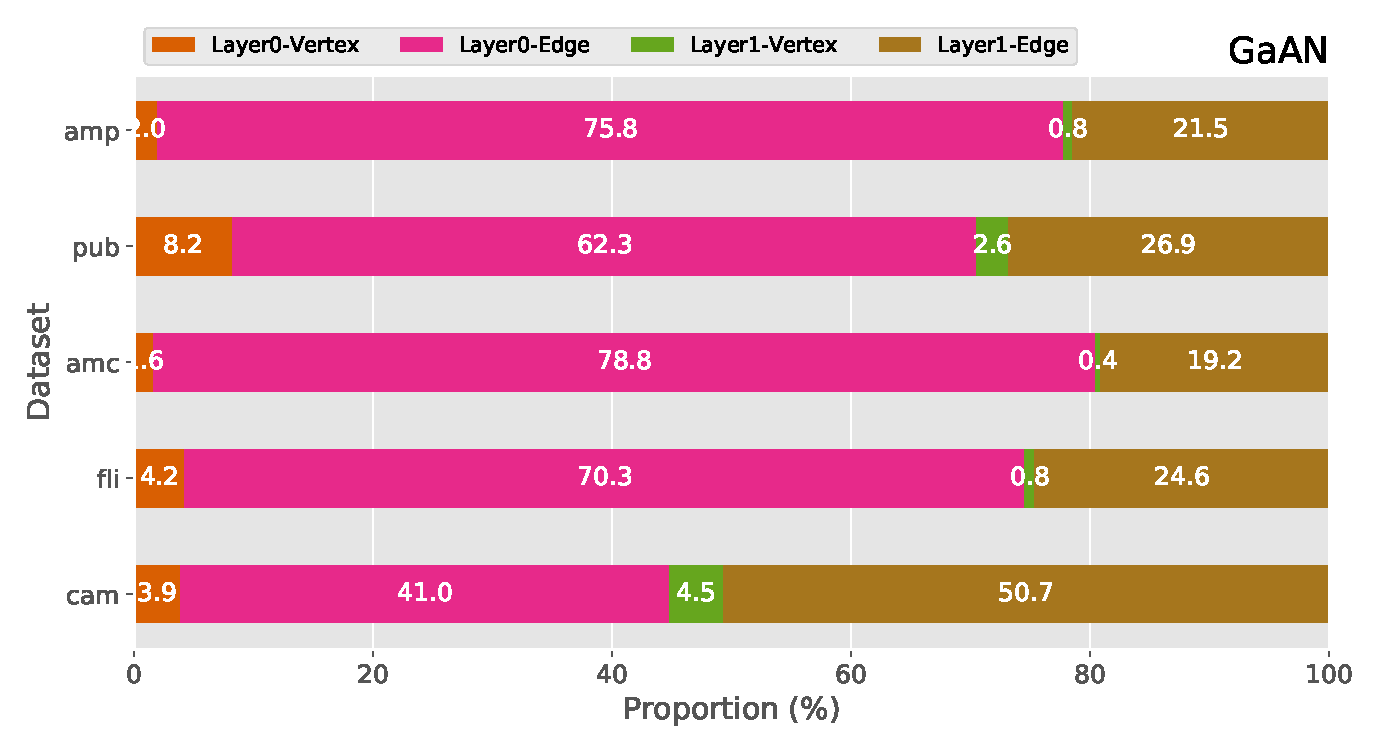
\includegraphics[height=4.6cm]{figs/experiments/exp_layer_time_proportion_gaan.pdf}}
    \caption{Training time breakdown on the layer level. The training time of each layer included the time spent on the forward, backward and evaluation phases. Each layer was further decomposed into the vertex and the edge calculation stages.}
    \label{fig:exp_vertex_edge_cal_proportion}
\end{figure}

Each GNN layer was further divided into the vertex and the edge calculation stages.
%
In \figurename~\ref{fig:exp_vertex_edge_cal_proportion}, GCN spent most of the training time on the edge calculation stage on most datasets.
%
A special case was the \texttt{cph} dataset.
%
The dimension of the input feature vectors was very high in \texttt{cph}, making the vertex calculation stage of the GCN Layer 0 spend considerable time.
%
GGNN also spent the majority of its training time on the edge calculation stage, but the high time complexity of its vertex updating function $\gamma^l$ made the proportion of the vertex calculation in the total training time much higher than the other GNNs.
%
For GAT and GaAN, due to their high edge calculation complexity, the edge calculation stage was the dominant stage.

The experimental results also indicated that the average degree of the dataset affected the proportion of the edge/vertex calculation time in the total training time.
%
For GaAN, the time spent on the vertex calculation stage exceeded the edge calculation stage on the \texttt{pub} and \texttt{cam} datasets, because the average degrees of the two datasets were low, making $|\mathcal{E}|$ and $|\mathcal{V}|$ much closer.
%
To evaluate the effects of the average degree, we generated random graphs with 50,000 vertices and average degrees ranging from 2 to 100.
%
\figurename~\ref{fig:exp_avg_degree_on_vertex_edge_cal_time} shows the training time of the four GNNs under different average degrees.
%
As the average degree increased, the training time of the edge calculation stage grew \emph{linearly}.
%
For GCN, GAT, and GaAN, the edge calculation stage dominated the entire training time even when the average degrees were small.
%
Only for GGNN that had high vertex and low edge calculation complexity, the training time of the vertex calculation stage exceeded the edge calculation stage under low average degrees ($<5$).

In summary, \emph{the edge calculation stage was the most time-consuming stage in GNN training}.
%
Improving its efficiency is the key to reduce the GNN training time.

\begin{figure}[H]
    \centering
    \subfloat[GCN]{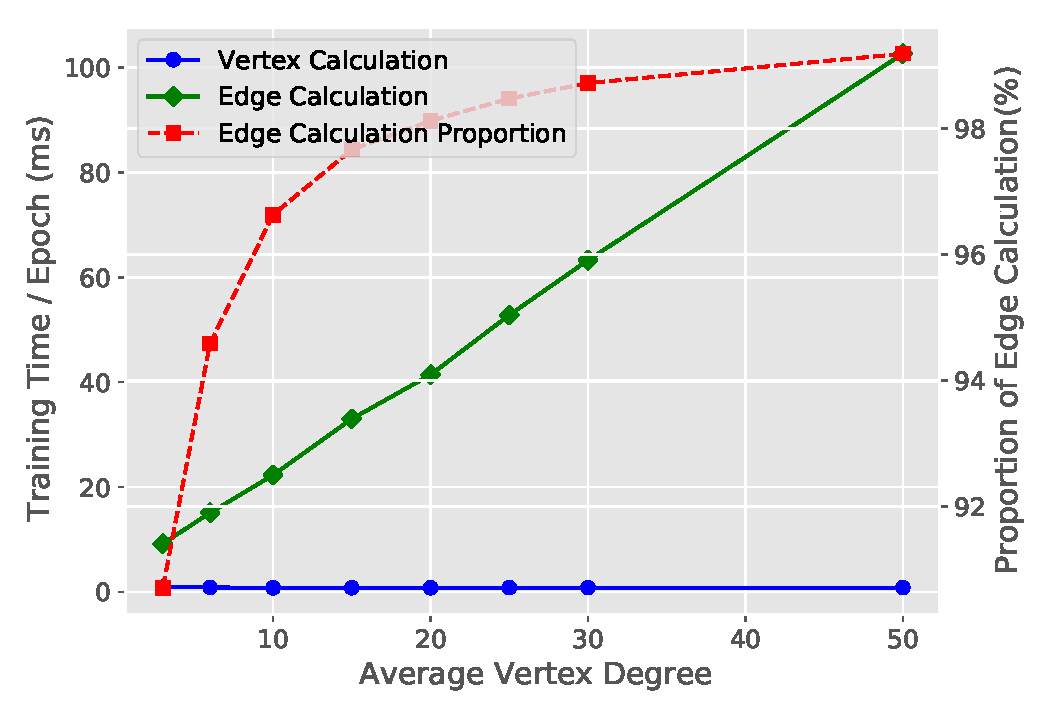
\includegraphics[height=4cm]{figs/experiments/exp_avg_degree_on_vertex_edge_cal_time_gcn.pdf}}
    \subfloat[GGNN]{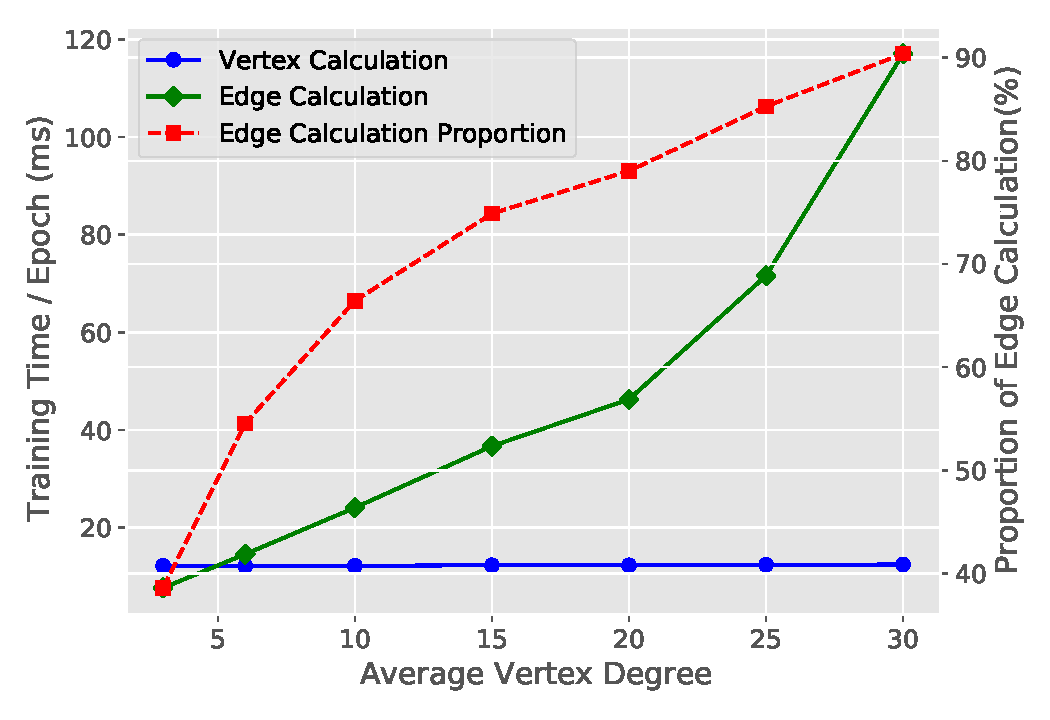
\includegraphics[height=4cm]{figs/experiments/exp_avg_degree_on_vertex_edge_cal_time_ggnn.pdf}}\\
    \subfloat[GAT]{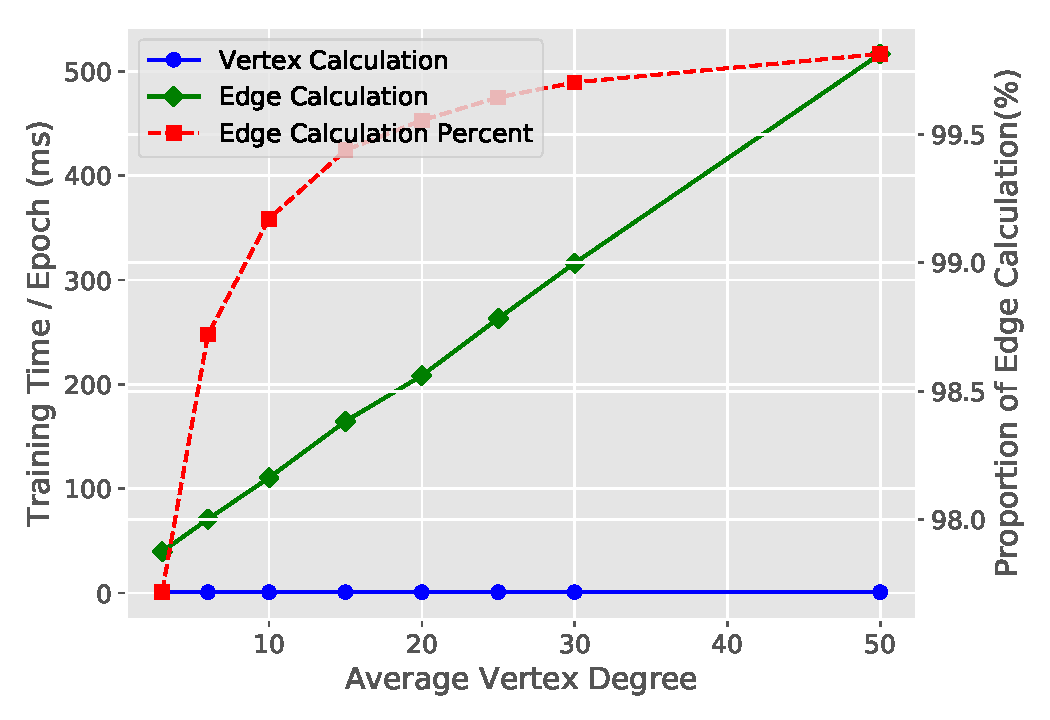
\includegraphics[height=4cm]{figs/experiments/exp_avg_degree_on_vertex_edge_cal_time_gat.pdf}}
    \subfloat[GaAN]{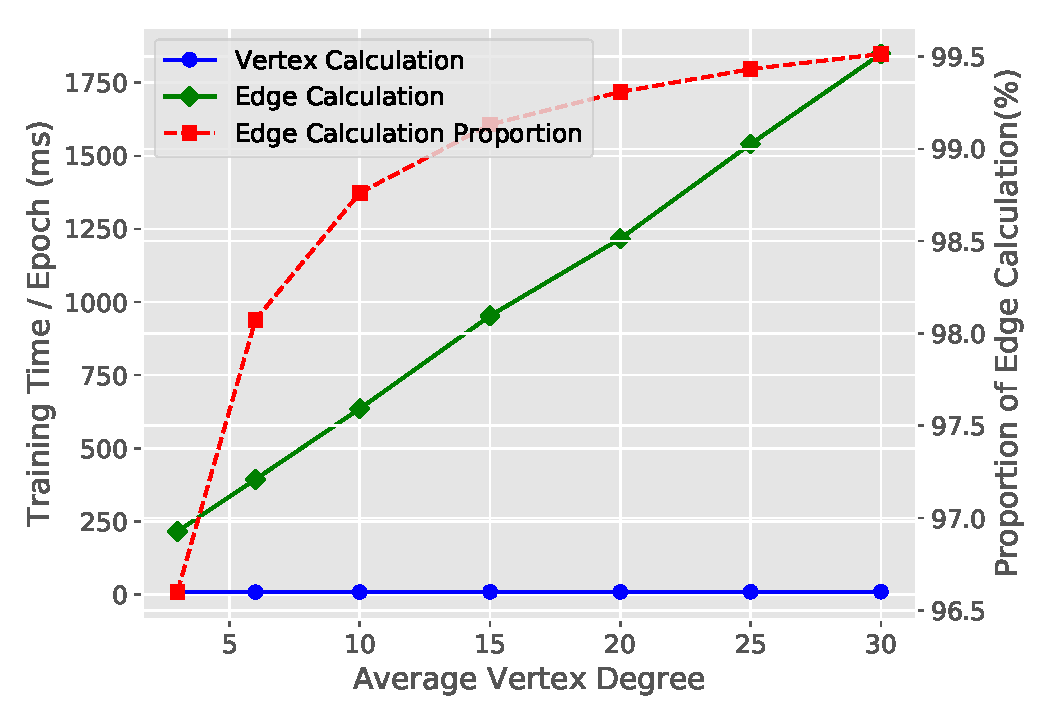
\includegraphics[height=4cm]{figs/experiments/exp_avg_degree_on_vertex_edge_cal_time_gaan.pdf}}
    \caption{Effects of the average degree on the time proportion of the edge/vertex calculation. Graphs were generated with the R-MAT generator by fixing the number of vertices as 50,000. }
    \label{fig:exp_avg_degree_on_vertex_edge_cal_time}
\end{figure}

\subsubsection{Step Level in Edge Calculation}

We further investigated the most time-consuming step of the edge calculation stage.
%
In the implementation of PyG, the edge calculation stage consists of four steps: collection, messaging, aggregation, and vector updating, as shown in \figurename~\ref{fig:steps_in_edge_calculation}.
%
The edge index is a matrix with $|\mathcal{E}|$ rows and two columns.
%
It holds the edge set of the graph.
%
The two columns of the edge index store the source and the target vertex IDs of each edge.
%
The collection step copies the hidden vectors from the previous GNN layer $\MyVec{h}^l_x$ and $\MyVec{h}^l_y$ to the both endpoints of each edge $e_{x,y}$ in the edge index, forming the parameter tensor $[\MyVec{h}^l_x, \MyVec{h}^l_{y}, \MyVec{e}_{x,y}]$ of the messaging function $\phi^l$.
%
This step only involves data movement.
%
The messaging step calls the messaging function $\phi^l$ on all edges to get message vectors $\MyVec{m}^l_{x,y}$.
%
The aggregation step aggregates the message vectors with the same target vertex into an aggregated vector $\MyVec{s}^l_x$.
%
The vector updating step is optional.
%
It performs an additional transformation on the aggregated vectors (for example, adding the bias in GCN).

\begin{figure}[H]
    \centering
    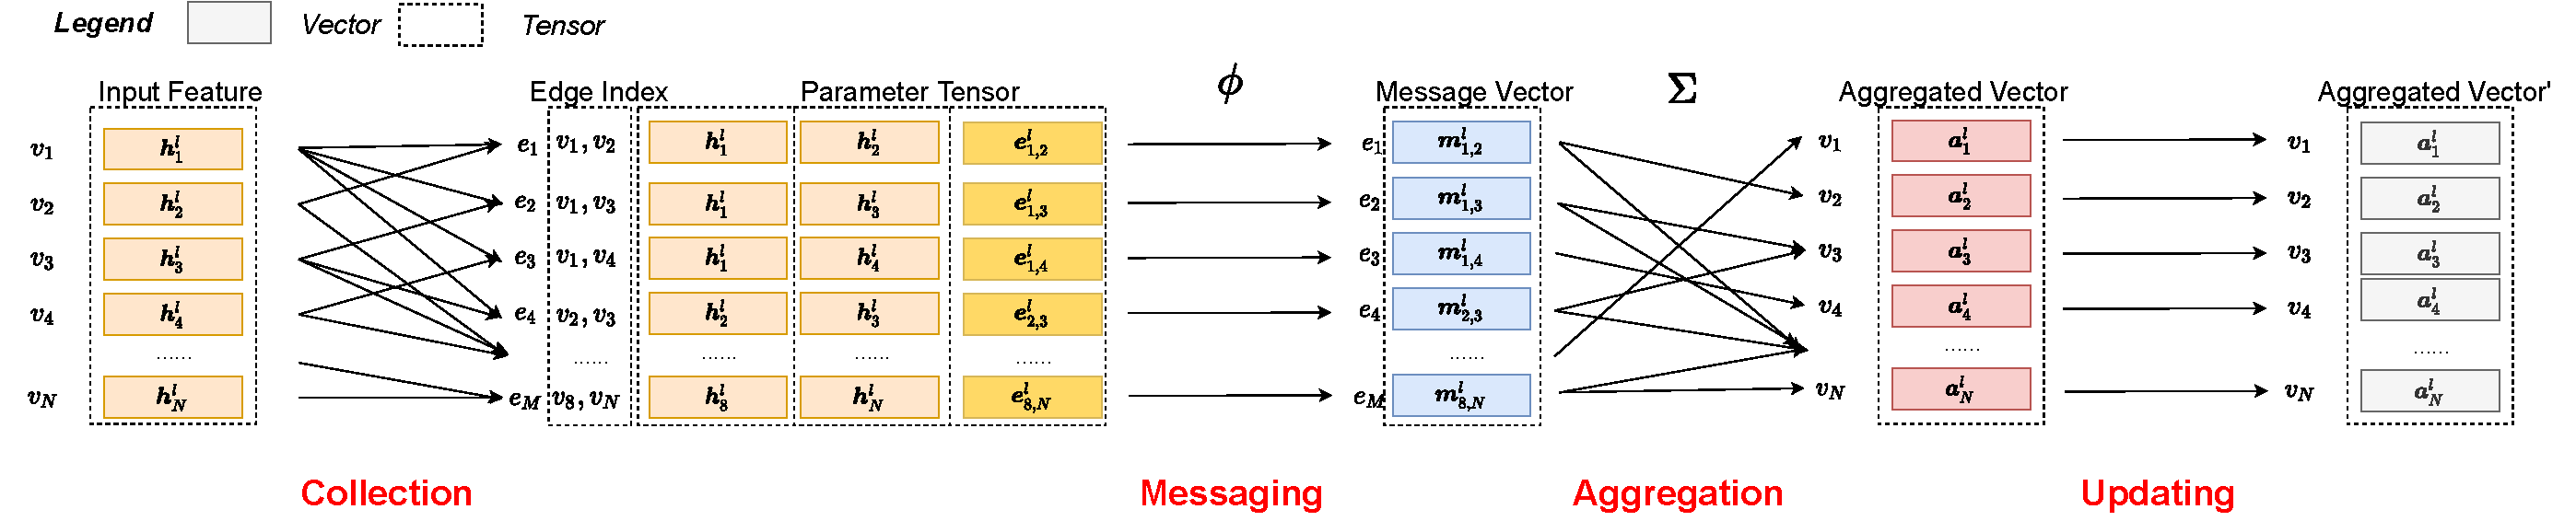
\includegraphics[width=1\columnwidth]{figs/illustration/steps_in_edge_calculation.pdf}
    \caption{Step decomposition of the edge calculation stage of the GNN layer $l$.}
    \label{fig:steps_in_edge_calculation}
\end{figure}

We decomposed the execution time of the edge calculation stage in \figurename~\ref{fig:exp_edge_calc_decomposition}.
%
In each GNN, the proportions of the four steps were rather stable, rarely affected by datasets. 
%
For GAT and GaAN with the high edge calculation complexity, the messaging step consumed most of the training time. 
%
For GCN and GGNN with the low edge complexity, the proportions of the steps were close. 
%
Since the messaging function $\phi^l$ of GGNN used the pre-computed $\MyVec{\hat{h}}^l_y$ as the message vector directly, the time spent on the messaging step of GGNN was negligible.
%
Although the collecting step did not conduct any computation and only involved data movement, it occupied noticeable execution time in the four GNNs.

The results indicate that \emph{the performance bottlenecks of the edge calculation stage depend on the complexity of the messaging function $\phi^l$}.
%
When the time complexity of $\phi^l$ is high, the messaging step is the performance bottleneck.
%
Optimizing the implementation of $\phi$ can significantly reduce training time.
%
Otherwise, the collection and the aggregation steps are performance bottlenecks.
%
Improving the efficiency of the two steps can benefit all GNNs.

\begin{figure}[H]
    \centering
    \subfloat[GCN]{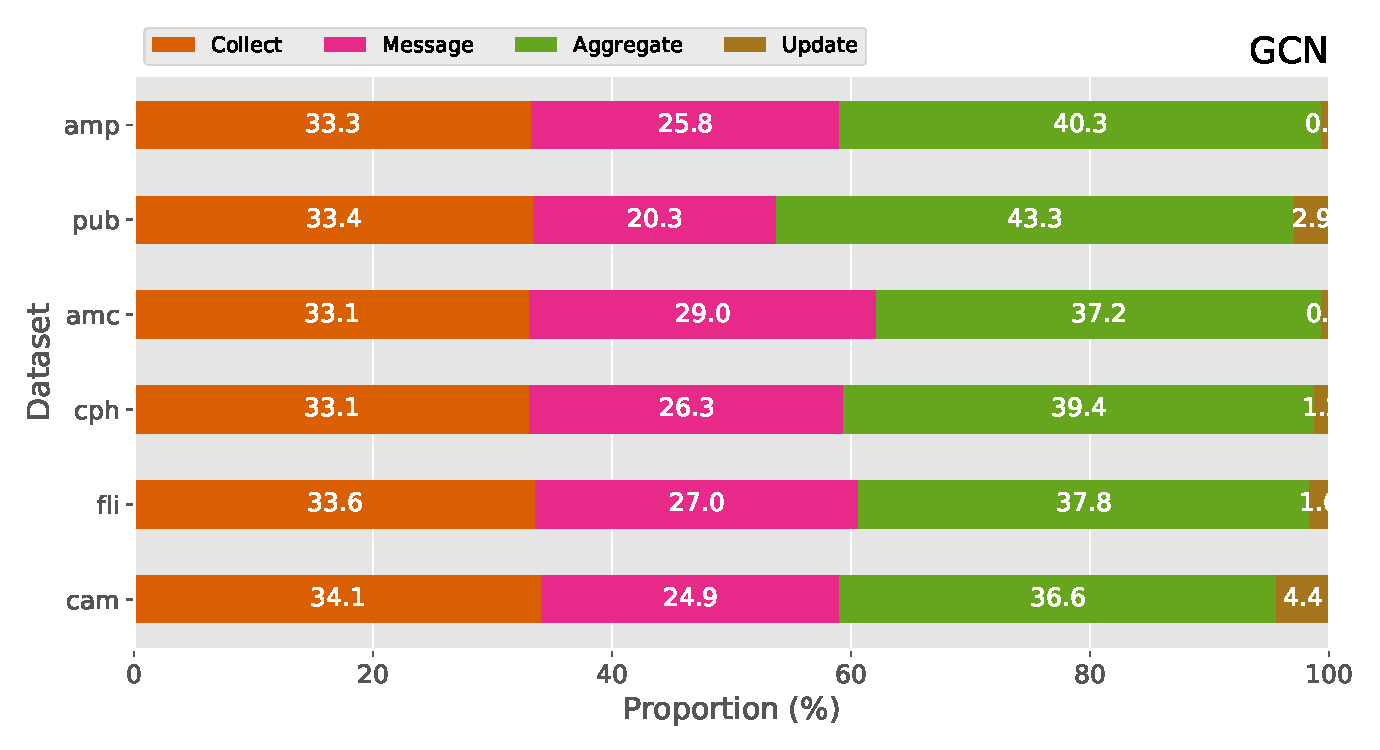
\includegraphics[height=4cm]{figs/experiments/exp_edge_calc_decomposition_gcn.pdf}}
    \subfloat[GGNN]{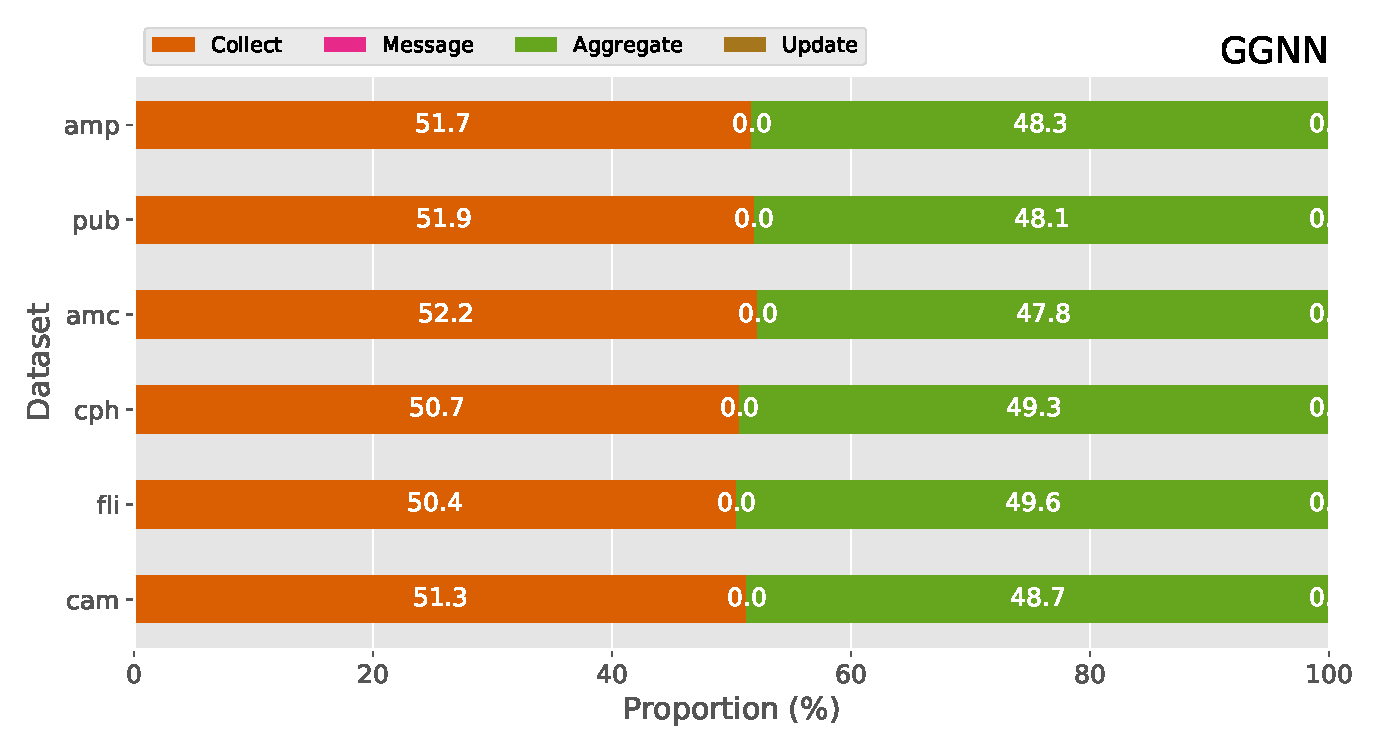
\includegraphics[height=4cm]{figs/experiments/exp_edge_calc_decomposition_ggnn.pdf}}\\
    \subfloat[GAT]{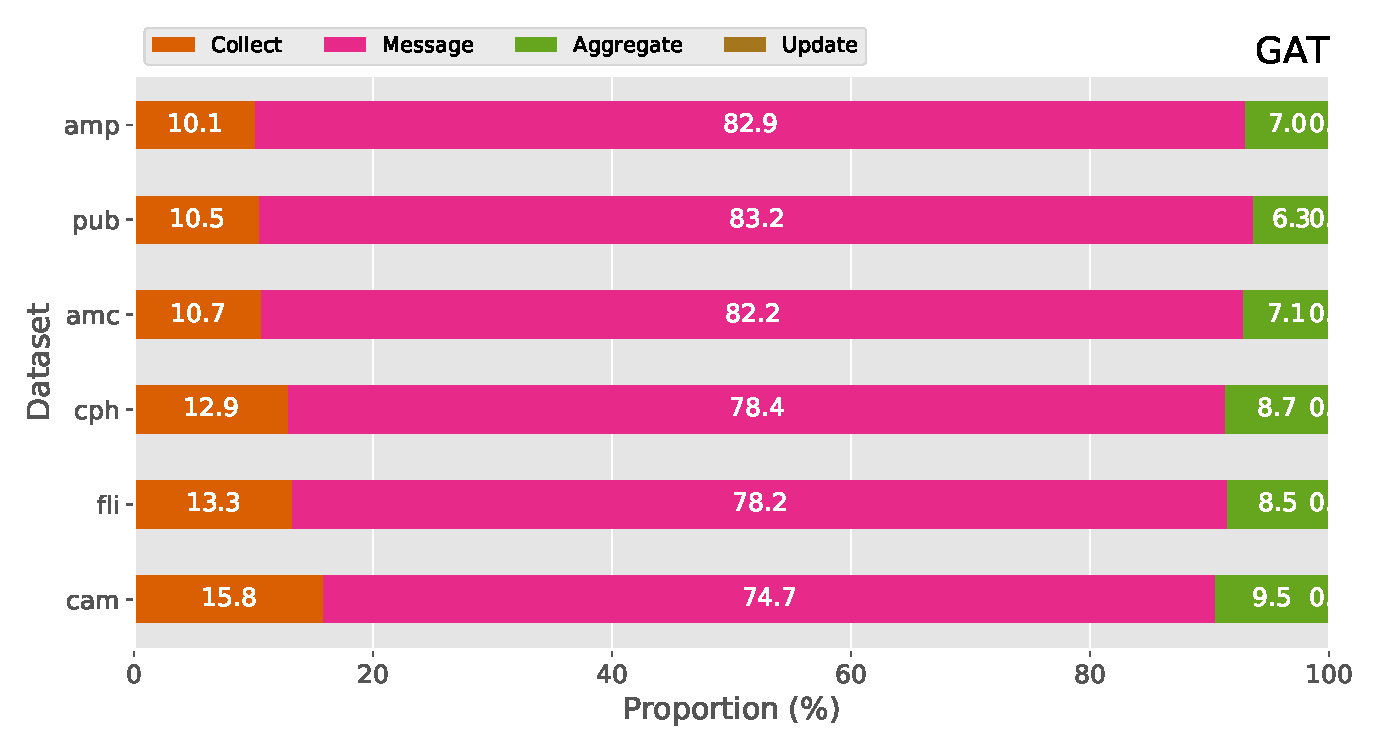
\includegraphics[height=4cm]{figs/experiments/exp_edge_calc_decomposition_gat.pdf}}
    \subfloat[GaAN]{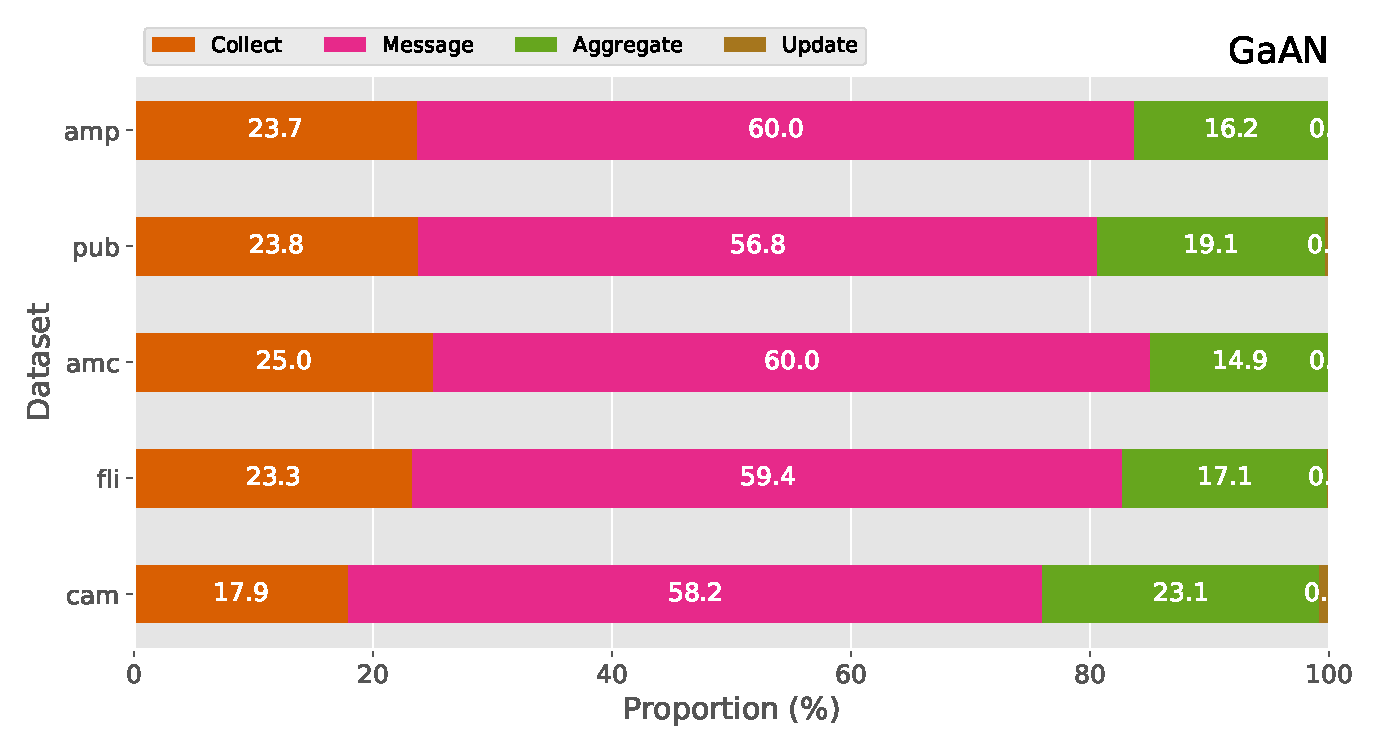
\includegraphics[height=4cm]{figs/experiments/exp_edge_calc_decomposition_gaan.pdf}}
    \caption{Training time breakdown of the edge calculation stage.}
    \label{fig:exp_edge_calc_decomposition}
\end{figure}

\subsubsection{Operator Level}

The functions $\phi$, $\Sigma$ and $\gamma$ in the edge and vertex calculation stages are made up of a series of basic operators implemented on the GPU side, such as the matrix multiplication \texttt{mm}, the elementwise multiplication \texttt{mul} and the index-based selection \texttt{index\_select}.
%
\figurename~\ref{fig:exp_top_basic_ops} shows the top-5 time-consuming basic operators in each GNN, averaged over all datasets.

\begin{figure}[H]
    \centering
    \subfloat[GCN]{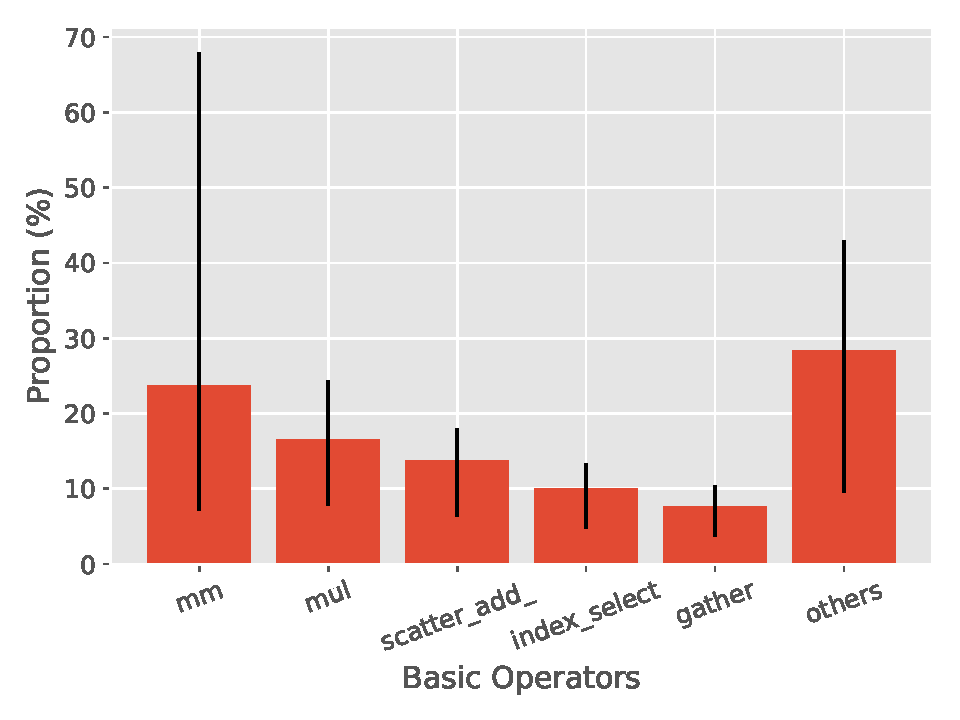
\includegraphics[height=4cm]{figs/experiments/exp_top_basic_ops_gcn.pdf}}
    \subfloat[GGNN]{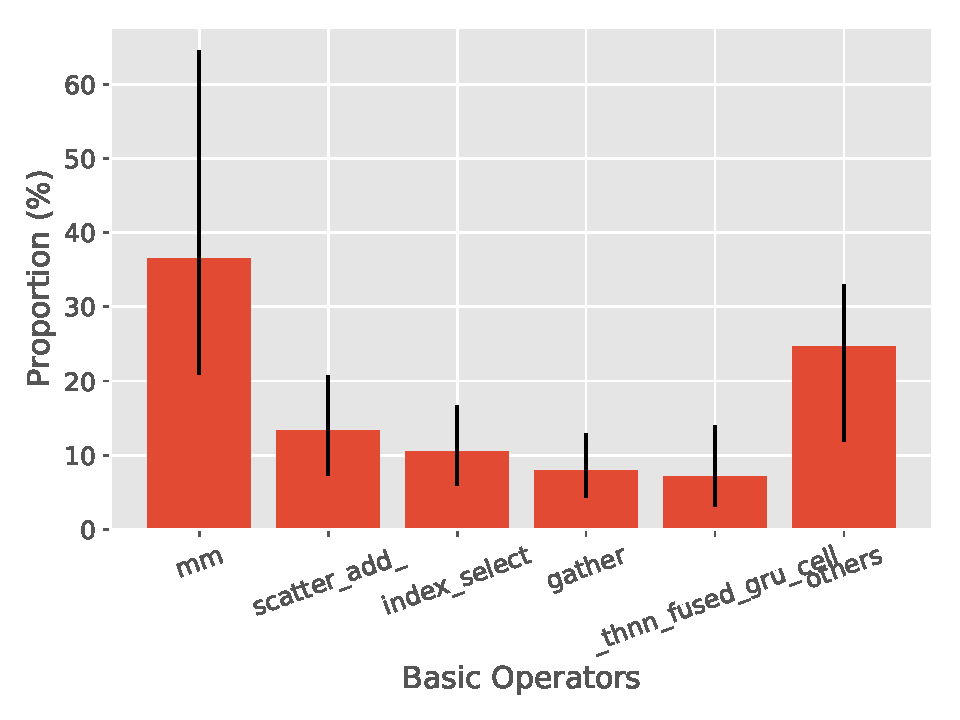
\includegraphics[height=4cm]{figs/experiments/exp_top_basic_ops_ggnn.pdf}}\\
    \subfloat[GAT]{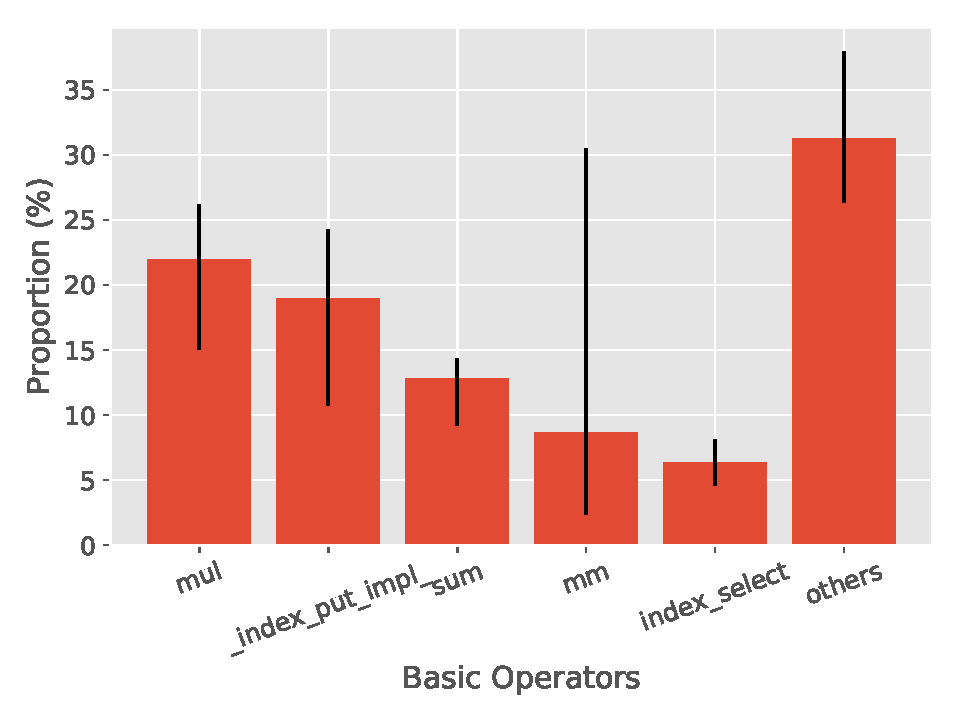
\includegraphics[height=4cm]{figs/experiments/exp_top_basic_ops_gat.pdf}}
    \subfloat[GaAN]{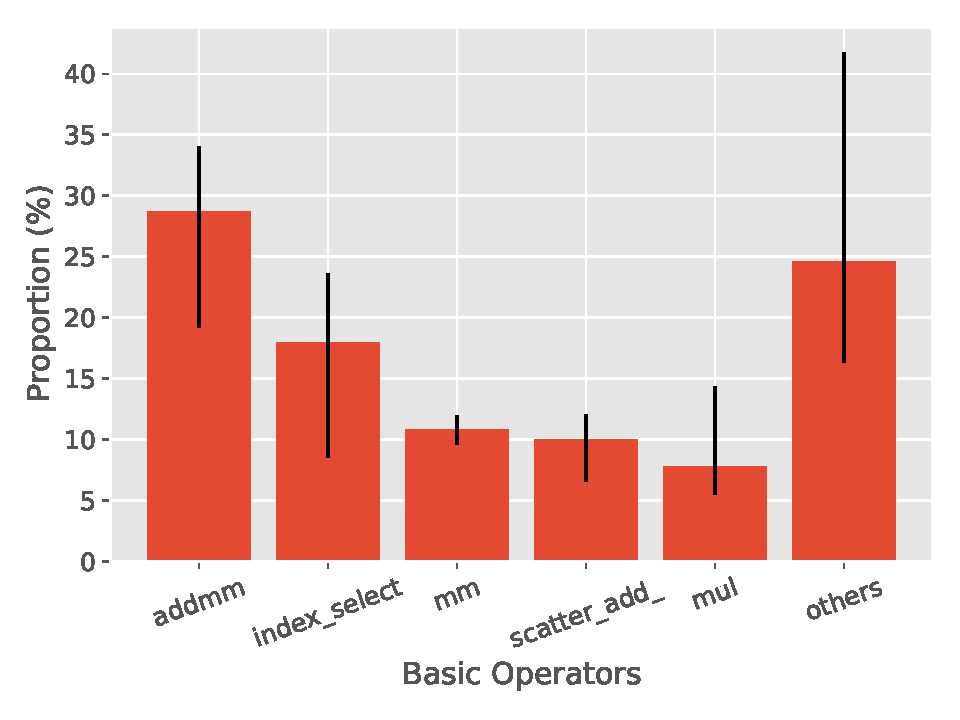
\includegraphics[height=4cm]{figs/experiments/exp_top_basic_ops_gaan.pdf}}
    \caption{Top 5 time-consuming basic operators of typical GNNs. The time proportion of each basic operator was averaged over all datasets with the error bar indicating the maximum and the minimum.}
    \label{fig:exp_top_basic_ops}
\end{figure}

\paragraph{GCN}
%
The most time-consuming basic operator was the matrix multiplication \texttt{mm} used in the vertex updating function $\gamma$.
%
The elementwise multiplication \texttt{mul} used in the messaging function $\phi$ was also time-consuming.
%
The other three operators were used in the edge calculation stage: \texttt{scatter\_add\_} for the aggregation step in the forward phase, \texttt{gather} for the aggregation step in the backward phase, and \texttt{index\_select} for the collection step.
%
For GCN, the basic operators related to the edge calculation stage consumed the majority of the training time.

\paragraph{GGNN}
%
The top basic operator was \texttt{mm} used in the vertex updating function $\gamma$.
%
Due to its high time complexity, the proportion of \texttt{mm} was much higher than the other operators.
%
The \texttt{thnn\_fused\_gru\_cell} operator was used in the backward phase of $\gamma$.
%
The other three operators were used in the edge calculation stage.

\paragraph{GAT}
%
All the top basic operators except for \texttt{mm} were related to the edge calculation stage.
%
The \texttt{mm} operator was used in the vertex updating function $\gamma$.

\paragraph{GaAN}
%
The top basic operator was \texttt{bmm} used in the messaging function $\phi$.
%
The \texttt{addmm} operator and the \texttt{mm} operator were used in both the vertex and the edge calculation stages, where the edge calculation stage was dominant.

The most time-consuming operators in the four GNNs were the matrix multiplication \texttt{mm} and the elementwise multiplication \texttt{mul}, \emph{making GNN training suitable for GPUs}.
%
Although the aggregation step in the edge calculation stage was relatively simple (like sum and mean), the related operators--\texttt{scatter\_add} and \texttt{gather}--still consumed a certain amount of the time.
%
The two operators had to synchronize between hardware threads to avoid updating the same aggregated vector at the same time.
%
They also conducted non-regular memory access with the access pattern determined by the edge set dynamically.
%
For GPUs, they were less efficient than \texttt{mm}.
%
The index-based selection operator \texttt{index\_select} used in the collection step consumed about 10\% of the training time in all GNNs.
%
Improving the efficiency of \texttt{scatter\_add}/\texttt{gather}/\texttt{index\_select} can benefit all kinds of GNNs.

\paragraph{Summary of Training Time Breakdown}
%
The GNN training was suitable for GPUs.
%
\emph{The edge calculation stage was the main performance bottleneck in most cases}, except for training GNNs with high vertex calculation complexity on low-average-degree graphs.
%
The performance bottleneck in the edge calculation stage depended on the time complexity of the messaging function $\phi$.
%
If the time complexity of $\phi$ was {high}, {$\phi$} dominated the training time of the edge calculation stage.
%
Optimizations should focus on improving its efficiency.
%
Otherwise, the {collection step} and the {aggregation step} dominated the training time.
%
The collection step suffered from lots of data movement.
%
The aggregation step suffered from data synchronization and non-regular data access.

\subsection{Inference Time Breakdown Analysis}
% 该部分

%

\subsection{Memory Usage Analysis}
\label{sec:memory_usage_analysis}

During the GNN training, we stored all data (including datasets and intermediate results) in the on-chip memory of the GPU.
%
Compared with the main memory on the host side (90 GB), the capacity of the GPU memory (16 GB) was very limited.
%
\emph{The GPU memory capacity limited the scales of the graphs that it could handle}.
%
For example, GaAN was unable to train on the \texttt{cph} dataset due to the out of memory exception.

\figurename~\ref{fig:exp_memory_usage_stage_amp} shows the peak memory usage of each phase during the GNN training on the \texttt{amp} dataset.
%
The trends on the other datasets were similar.
%
\emph{The GNN training achieved its peak memory usage in the forward and the backward phases}.
%
The forward phase generated lots of intermediate results.
%
Some key intermediate results were cached for the gradient calculation in the backward phase, increasing memory usage.
%
For example, \figurename~\ref{fig:ggnn_vertex_func_computation_graph} shows the computation graph of the vertex updating function $\gamma^l$ of GGNN.
%
Each operator in the computation graph generated an intermediate tensor.
%
Some key intermediate tensors are cached.
%
The cached tensors were the main source of memory usage in the loss phase.
%
By the end of the backward phase, the cached tensors were released.
%
Since the evaluation phase did not have to calculate the gradients, it did not cache intermediate tensors.
%
Its memory usage declined sharply.

\begin{figure}[H]
    \centering
    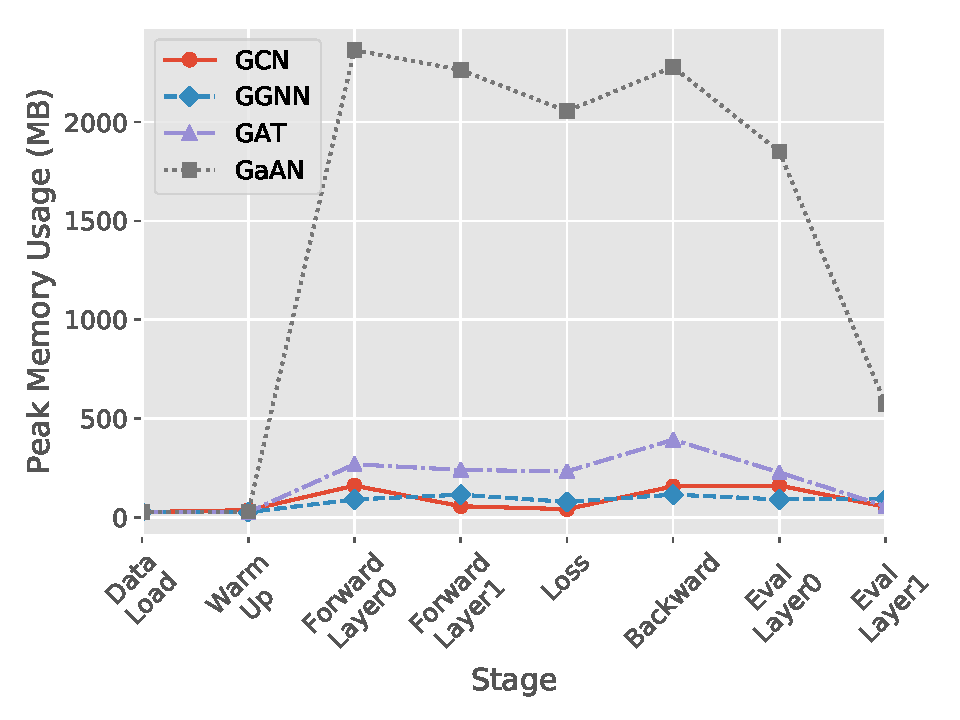
\includegraphics[height=5cm]{figs/experiments/exp_memory_usage_stage_amp.pdf}
    \caption{Memory usage of each phase during the GNN training. Dataset: \texttt{amp}.}
    \label{fig:exp_memory_usage_stage_amp}
\end{figure}

\begin{figure}[H]
    \centering
    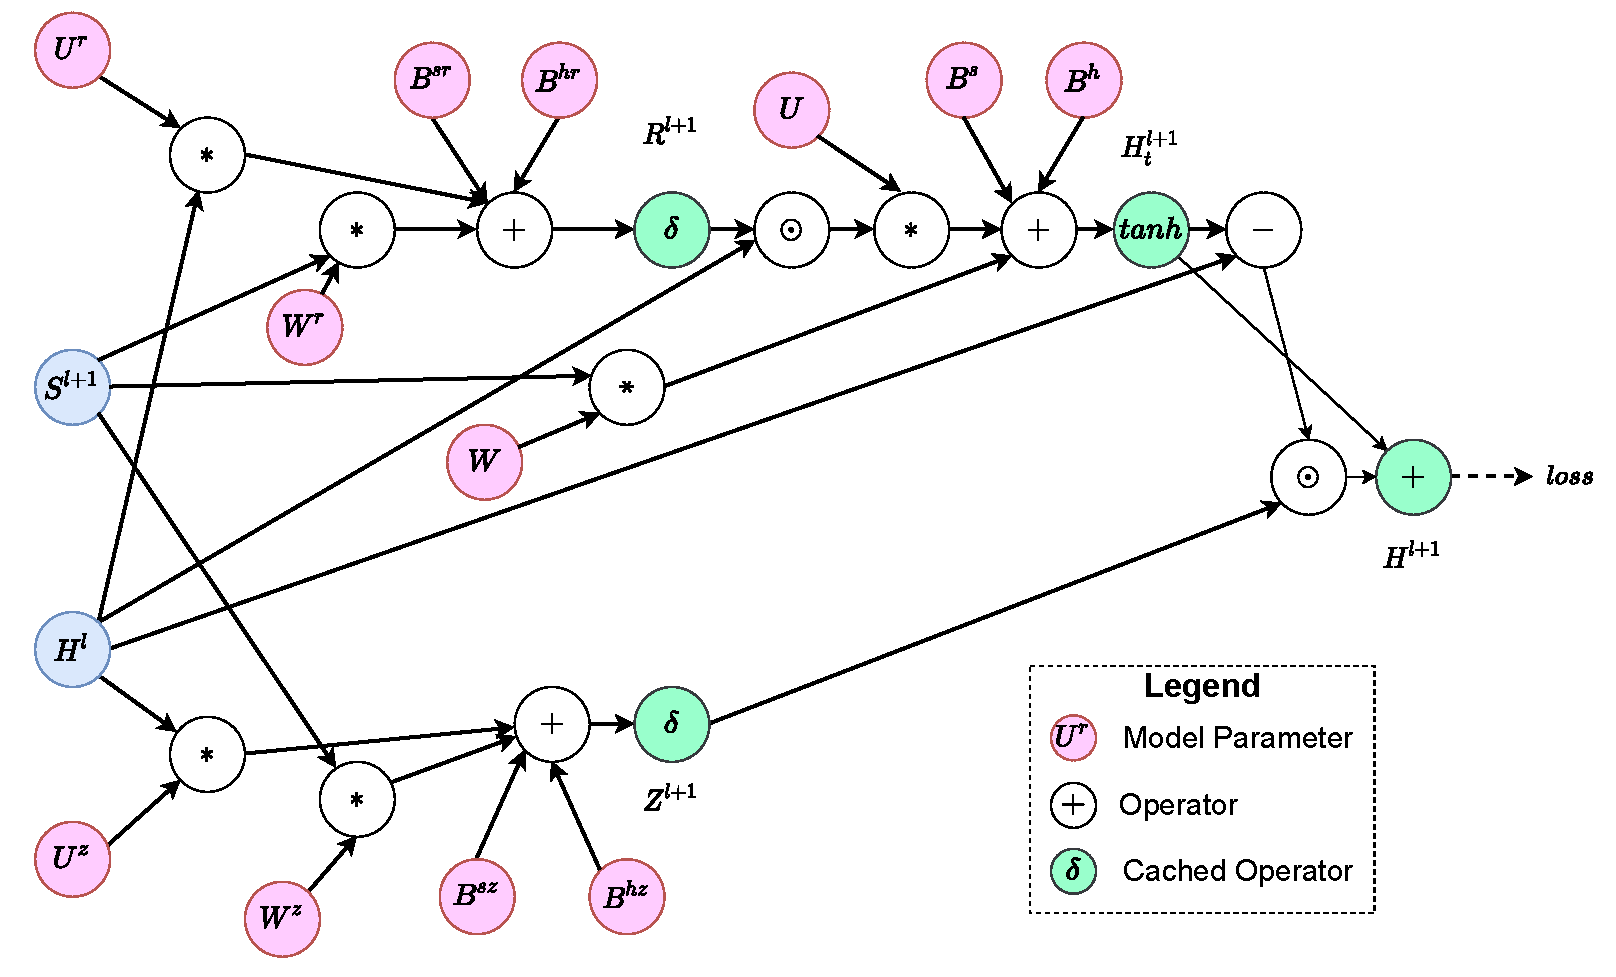
\includegraphics[width=0.7\columnwidth]{figs/illustration/ggnn_vertex_func_computation_graph.pdf}
    \caption{Computation graph of the vertex updating function $\gamma$ of GGNN.}
    \label{fig:ggnn_vertex_func_computation_graph}
\end{figure}

The peak memory usage during the GNN training far exceeded the size of the dataset itself.
%
We defined the \emph{memory expansion ratio} (MER) as the ratio of the peak memory usage during the training to the memory usage after loading the dataset.
%
\figurename~\ref{fig:exp_memory_expansion_ratio} compares MER of different GNNs.
%
GCN had the lowest MER (up to 15) while GaAN had the highest MER (up to 104).
%
\emph{The high MERs limited the data scalability of GNNs}, making GPUs unable to handle big graphs.
%
\figurename~\ref{fig:exp_memory_expansion_ratio} also indicates that the same GNN had different MERs for different datasets.
%
Two characteristics of a dataset affected the MER: the dimension of the input feature vectors and the average degree of the graph.

\begin{figure}[H]
    \centering
    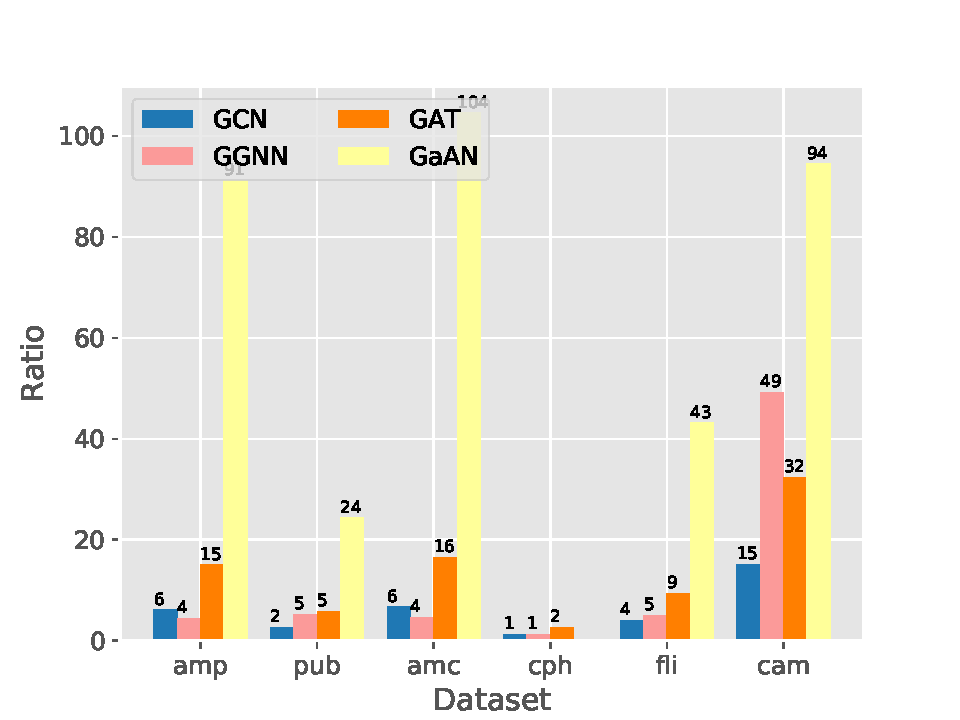
\includegraphics[width=0.5\columnwidth]{figs/experiments/exp_memory_expansion_ratio.pdf}
    \caption{Memory expansion ratios of typical GNNs.}
    \label{fig:exp_memory_expansion_ratio}
\end{figure}

To find out how the dimension of input feature vectors affected the MER, we generated random input feature vectors with different dimensions for the \texttt{cam} dataset and measured the MER in \figurename~\ref{fig:exp_memory_expension_ratio_input_feature_dimension}.
%
Under the same hyper-parameters, \emph{the MER decreased as the dimension of input feature vectors increased}.
%
When the dimension of the input feature vectors was high, the size of the dataset itself was large.
%
The size became comparable to the size of intermediate results,  making MERs low.


\begin{figure}[H]
    \centering
    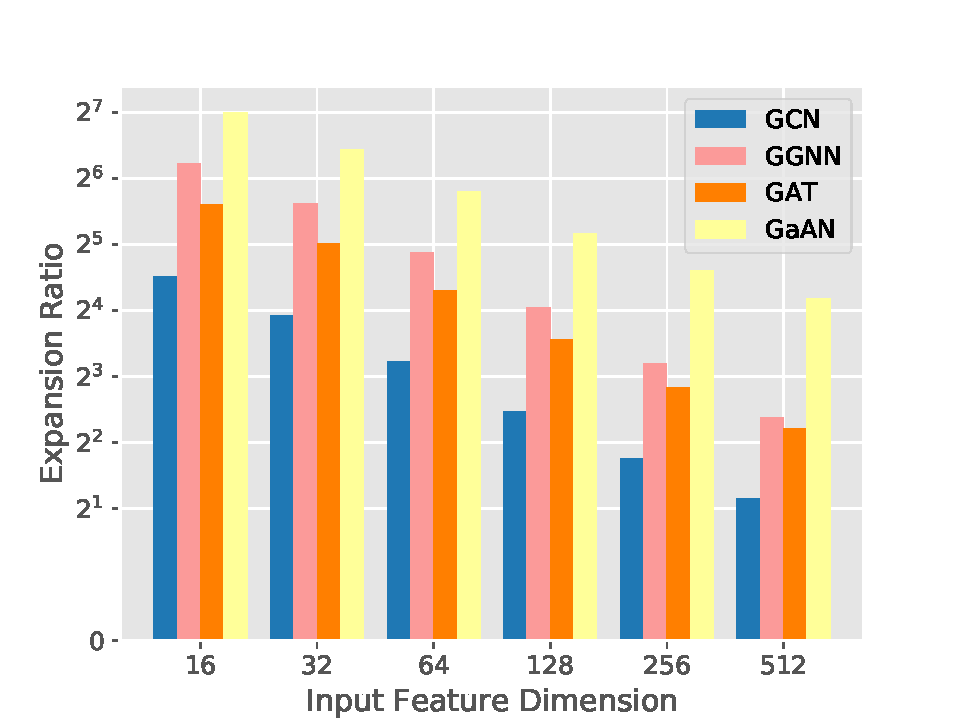
\includegraphics[height=5cm]{figs/experiments/exp_memory_expansion_ratio_input_feature_dimension_com-amazon.pdf}
    \caption{Memory expansion ratio under different dimensions of input feature vectors. Dataset: \texttt{cam}.}
    \label{fig:exp_memory_expension_ratio_input_feature_dimension}
\end{figure}

Average degrees also affected MERs by influencing the relative sizes of intermediate results from the edge and the vertex calculation stages.
%
Fixing the number of vertices $|\mathcal{V}|$, we generated random graphs with different average degrees.
%
\figurename~\ref{fig:exp_memory_expansion_ratio_input_graph_number_of_edges} shows how the memory usage changed according to the average degree.
%
As the average degree $\bar{d}$ increased, the peak memory usage increased \emph{linearly} with $\bar{d}$.
%
The edge calculation stage gradually dominated the memory usage and \emph{the MER converged to a stable value}.
%
The stable value was determined by the complexity of the edge calculation stage.
%
Except for GGNN, the MERs of the other GNNs increased as $\bar{d}$ increased.
%
As GGNN had high vertex calculation complexity, the MERs related to the vertex calculation stage were much higher than the edge calculation stage.
%
When the edge calculation stage dominated the memory usage, its MERs became smaller.

\begin{figure}[H]
    \centering
    \subfloat[Peak memory usage]{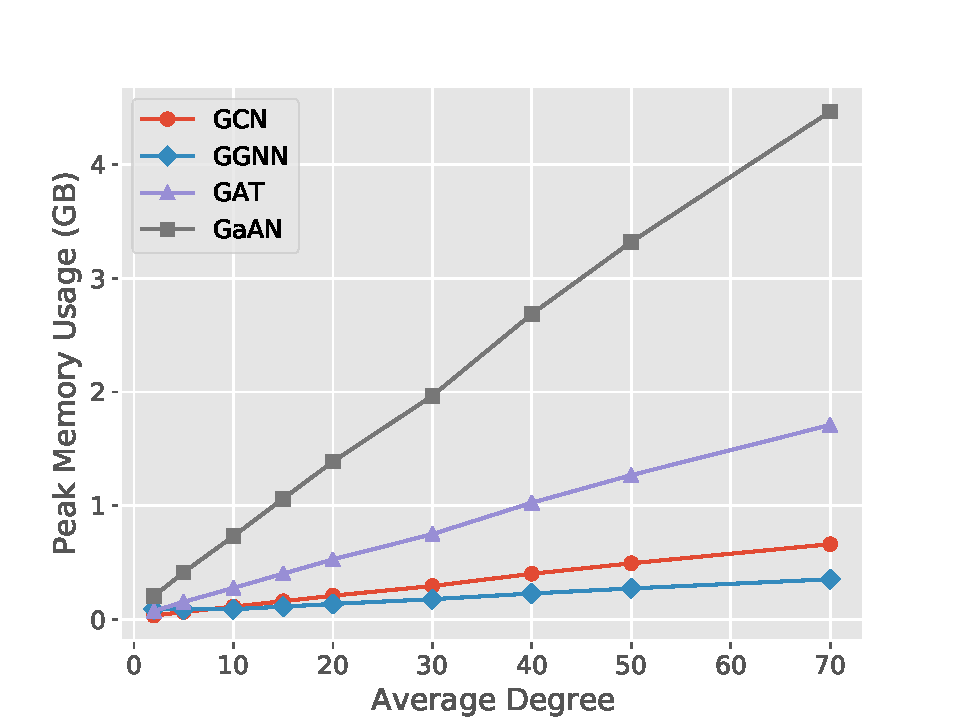
\includegraphics[height=4cm]{figs/experiments/exp_memory_expansion_ratio_input_graph_number_of_edges_peak_memory.pdf}}
    \subfloat[Memory expansion ratio]{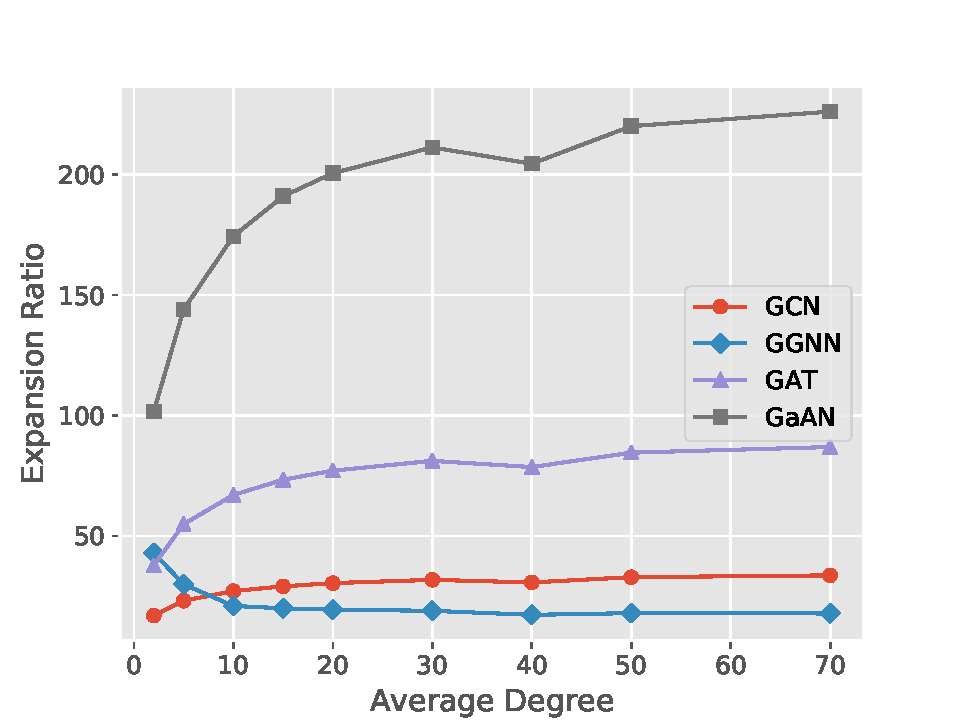
\includegraphics[height=4cm]{figs/experiments/exp_memory_expansion_ratio_input_graph_number_of_edges_expansion_ratio.pdf}}
    \caption{Memory usage under different average degrees. The random graphs were generated by fixing the number of vertices at 10K and the dimension of input feature vectors at 32.}
    \label{fig:exp_memory_expansion_ratio_input_graph_number_of_edges}
\end{figure}

We also fixed the number of edges $|\mathcal{E}|$ and generated random graphs with different $|\mathcal{V}|$.
%
\figurename~\ref{fig:exp_memory_expansion_ratio_input_graph_number_of_vertices_fixed_edge} shows how the memory usage changed according to $|\mathcal{V}|$.
%
MERs of all GNNs were insensitive to $|\mathcal{V}|$, compared to $|\mathcal{E}|$.
%
Except for GGNN, the MERs of the other GNNs declined as $|\mathcal{V}|$ increased because the sizes of the datasets increased more quickly than the sizes of the intermediate results.
%
As GGNN had high vertex calculation complexity, the sizes of the intermediate results were very sensitive to $|\mathcal{V}|$.
%
It indicated that \emph{the intermediate results of the edge calculation stage dominated the memory usage during the GNN training}.

\begin{figure}[H]
    \centering
    \subfloat[Peak memory usage]{\includegraphics[height=4cm]{figs/experiments/exp_memory_expansion_ratio_input_graph_number_of_vertices_fixed_edge_peak_memory.pdf}}
    \subfloat[Memory expansion ratio]{\includegraphics[height=4cm]{figs/experiments/exp_memory_expansion_ratio_input_graph_number_of_vertices_fixed_edge_expansion_ratio.pdf}}
    \caption{Memory usage under different numbers of vertices. The random graphs were generated by fixing the number of edges at 500K and the dimension of input feature vectors at 32.}
    \label{fig:exp_memory_expansion_ratio_input_graph_number_of_vertices_fixed_edge}
\end{figure}

\paragraph{Summary of Memory Usage}
%
The \emph{high} memory expansion ratio severely restricted the data scalability of GNN training.
%
The memory usage mainly came from the intermediate results of the \emph{edge calculation stage}.
%
Fixing the number of vertices, the memory usage increased \emph{linearly} along with the number of edges.
%
Fixing the GNN structure and the hyper-parameters, increasing the dimension of input feature vectors could reduce the memory expansion ratio.
%
To reduce the memory usage of GNN training, optimizations should focus on reducing memory footprints of the edge calculation stage.

\subsection{Effects of Sampling Techniques on Performance}
\label{sec:effects_of_sampling_techniques_on_performance}

With the sampling techniques, GNNs were trained in a mini-batch manner.
%
Each epoch was decomposed into many batches.
%
In each batch, PyG only sent the sampled subgraph to the GPU to train or inference.
%
Since the sampled subgraphs could be much smaller than the original graph, the experiments in this section focused on finding out how the sample size affected the training time, the memory usage and the accuracy of GNNs.

\figurename~\ref{fig:exp_sampling_minibatch_graph_info} shows how the size of the sampled subgraph changed with the batch size.
%
For the neighbor sampler, the relative batch size was defined as the proportion of the sampled vertices of the last GNN layer in $\mathcal{V}$.
%
For the cluster sampler, the relative batch size was defined as the proportion of the sampled partitions in all partitions of the graph.
%
The experimental results indicated that the neighbor sampler was very sensitive to the batch size.
%
As the batch size increased, the size of the sampled subgraph first increased quickly and then stabilized.
%
The cluster sampler was much less sensitive compared to the neighbor sampler.
%
The number of vertices and the average degree of the sampled subgraphs increased linearly with the batch size.

\begin{figure}[H]
    \centering
    \subfloat[Neighbor sampler]{\includegraphics[height=4cm]{figs/experiments/exp_sampling_minibatch_realtive_graph_info_graphsage_gcn.pdf}} \\
    \subfloat[Cluster sampler]{\includegraphics[height=4cm]{figs/experiments/exp_sampling_minibatch_realtive_graph_info_cluster_gcn.pdf}}
    \caption{Sizes of sampled subgraphs under different relative batch sizes. The batch size was relative to the full graph. Each batch size was sampled 50 times and the average values were reported. The error bar indicates the standard deviation.}
    \label{fig:exp_sampling_minibatch_graph_info}
\end{figure}

The average degree of the sampled subgraph was \emph{much lower} than the average degree of the original graph, especially when the relative batch size is low.
%
Taking the neighbor sampler with the relative batch size of 6\% as an example, the average degree of the \texttt{amp} dataset was 31.1, but the average degree of the sampled subgraph was only 5.8.
%
For the cluster sampler, the average degree was 3.0.
%
\figurename~\ref{fig:exp_sampling_minibatch_degrees_distribution} compares the degree distribution of the sampled subgraphs with the original graph.
%
The slopes of the curves were similar, indicating that the sampled subgraphs still followed the power-law degree distribution.
%
However, the numbers of high-degree vertices were much less than the original graph, lowering the average degrees.
%
According to the experimental results in Section~\ref{sec:training_time_breakdown}, if the average degree became lower, the proportion of the training time spent on the vertex calculation stage would become higher, especially for GGNN.

\begin{figure}[H]
    \centering
    \includegraphics[width=0.4\columnwidth]{figs/experiments/exp_sampling_minibatch_degrees_distribution_amazon-photo.pdf}
    \caption{Vertex degree distribution of the sampled subgraph (relative batch size: 6\%) and the original graph. Dataset:\texttt{amp}.}
    \label{fig:exp_sampling_minibatch_degrees_distribution}
\end{figure}

To find out performance bottlenecks of the sampling techniques, we decomposed the training time per batch into three phases: \emph{sampling} on the CPU side, \emph{transferring} sampled subgraphs from the CPU side to the GPU side, and \emph{training} with the sampled subgraphs on the GPU side.
%
\figurename~\ref{fig:exp_sampling_batch_train_time} shows the time breakdown of the four GNNs under different relative batch sizes.
%
For the neighbor sampler, the sampling technique reduced the training time per batch only when the batch size was very small.
%
When the batch became bigger, the sampling and the data transferring phases introduced noticeable overheads, making the training time exceed the full-batch training.
%
For the clustering sampler, the sampled subgraph was smaller than the neighbor sampler under the same relative batch size.
%
The reduction in the training time was more obvious than the neighbor sampler.
%
However, the overheads increased quickly as the relative batch size increased.
%
The training time under the 25\% relative batch size already exceeded the time of full-batch training.
%
The experimental results indicated that the current implementation of the sampling techniques in PyG was inefficient.
%
When the batch size was large, more than 50\% of the time had been spent on sampling and data transferring.
%
\emph{The sampling techniques were only efficient under small batch sizes.}


\begin{figure}[H]
    \centering
    \subfloat[Neighbor sampler on \texttt{amc}]{\includegraphics[height=5cm]{figs/experiments/exp_sampling_relative_batch_size_train_time_stack_graphsage_amazon-computers.pdf}}
    \subfloat[Neighbor sampler on \texttt{fli}]{\includegraphics[height=5cm]{figs/experiments/exp_sampling_relative_batch_size_train_time_stack_graphsage_flickr.pdf}} \\
    \subfloat[Cluster sampler on \texttt{amc}]{\includegraphics[height=5cm]{figs/experiments/exp_sampling_relative_batch_size_train_time_stack_cluster_amazon-computers.pdf}}
    \subfloat[Cluster sampler on \texttt{fli}]{\includegraphics[height=5cm]{figs/experiments/exp_sampling_relative_batch_size_train_time_stack_cluster_flickr.pdf}}
    \caption{Training time per batch breakdown. FULL means that the full graph participates in the training.}
    \label{fig:exp_sampling_batch_train_time}
\end{figure}

The main advantage of the sampling techniques was \emph{reducing the peak memory usage} during training.
%
\figurename~\ref{fig:exp_sampling_memory_usage} shows the memory usage under different batch sizes.
%
The peak memory usage declined significantly even under big batch sizes.
%
The sampling techniques made training GNNs on big graphs \emph{possible} for GPUs.

\begin{figure}[H]
    \centering
    \subfloat[Neighbor sampler on \texttt{amc}]{\includegraphics[height=4cm]{figs/experiments/exp_sampling_memory_usage_relative_batch_size_graphsage_amazon-computers_peak_memory.pdf}}
    \subfloat[Neighbor sampler on \texttt{fli}]{\includegraphics[height=4cm]{figs/experiments/exp_sampling_memory_usage_relative_batch_size_graphsage_flickr_peak_memory.pdf}} \\
    \subfloat[Cluster sampler on \texttt{amc}]{\includegraphics[height=4cm]{figs/experiments/exp_sampling_memory_usage_relative_batch_size_cluster_amazon-computers_peak_memory.pdf}}
    \subfloat[Cluster sampler on \texttt{fli}]{\includegraphics[height=4cm]{figs/experiments/exp_sampling_memory_usage_relative_batch_size_cluster_flickr_peak_memory.pdf}}
    \caption{Peak memory usage under different batch sizes. FULL means that the full graph participated in the training.}
    \label{fig:exp_sampling_memory_usage}
\end{figure}

The disadvantage of the sampling technique was wasting GPU resources.
%
As the sampling techniques were only effective under small batch sizes, the sampled subgraphs were very small in those cases.
%
They could not make full use of the computing power of a GPU.
%
To simulate the situation, we generated random graphs with few vertices and measured their training time per epoch in \figurename~\ref{fig:exp_small_graph_train_time}.
%
As the number of vertices increased, the training time was almost unchanged except for GaAN.
%
The training time of GaAN increased only when $|\mathcal{V}| \geq 4000$.

\begin{figure}[H]
    \centering
    \includegraphics[height=5cm]{figs/experiments/exp_small_graph_train_time.pdf}
    \caption{Training time per epoch on small random graphs. For each number of vertices, we generated 50 random graphs with the average degree of 4.0 and reported the average training time per batch (without the evaluation phase). The error bar indicates the standard deviation.}
    \label{fig:exp_small_graph_train_time}
\end{figure}

\paragraph{Summary of Sampling Techniques}

The sampled subgraphs had lower average degrees than the original graph.
%
With small batch sizes, the sampling techniques could significantly reduce the training time per batch and the peak memory usage.
%
However, small batch sizes could not make full use of the computing power of a GPU.
%
With big batch sizes, the current implementation of the sampling techniques in PyG was inefficient.
%
The time spent on the sampling phase and the data transferring phase even exceeded the training phase.

\section{Insights}
\label{sec:insights}

Through the extensive experiments, we propose the following key findings/suggestions for how to optimize the performance of GNN training.

\begin{enumerate}
    \item \emph{The time complexity in \tablename~\ref{tab:gnn_overview_edge} and \tablename~\ref{tab:gnn_overview_vertex} points out the performance bottleneck theoretically.}
          The experimental results validate the time complexity analysis.
          The time complexity points out where the bottleneck comes from.
          Optimization should focus on complex operations in $\phi$ and $\gamma$.

    \item \emph{The computational cost of a GNN layer is mainly affected by the dimensions of the input and the output hidden feature vectors.}
          Theoretically and empirically, the training time and the memory usage both increase \emph{linearly} with the dimensions of the hidden feature vectors.
          GNNs are friendly to high-dimensional scenarios.
          Algorithm engineers can use high-dimensional feature vectors to improve the expressive power of a GNN without worrying explosive growth in the training time and memory usage.

    \item \emph{Performance optimizations should focus on improving the efficiency of the edge calculation.}
          The edge calculation is the most time-consuming phase in most GNNs.
          \begin{itemize}
              \item If the complexity of the message function $\phi$ is high, the implementation of $\phi$ is critical to performance.
                    Improving its efficiency can significantly reduce training time.
                    For example, the attention mechanism in GNNs (like GAT and GaAN) requires an extra sub-layer to calculate the attention weight of each edge.
                    Implementing it with the specially optimized basic operators on GPU is a potential optimization.
              \item If the complexity of $\phi$ is low, the efficiency of the collect step and the aggregation step becomes critical.
                    The existing GNN libraries \cite{DGL, PyG, ma2019_neugraph} already introduce the \emph{fused} operator to improve their efficiency.
                    When the message function $\phi$ is an assignment or a scalar multiplication of the hidden feature vector of the source vertex, the libraries replace the collect, message, and aggregate steps with a single fused operator.
                    The fused operator calculates the aggregated vectors directly from the input hidden feature vectors, minimizing the memory footprints and overlapping the memory accessing with calculation.
                    In this way, it significantly reduces the training time of GNNs with low edge calculation complexity (like GCN) \cite{yan2020_characterizing_gcn, zhang2020_analysis_neugraph}.
                    However, the applicable condition of the fused operator is very restricted.
                    It does not work for $\phi$ with more complex operations like matrix multiplication.
                    A potential optimization is proposing an implementation of the edge calculation that generates the aggregated vectors directly from the input hidden feature vectors on the fly, without materializing the parameter vectors and the message vectors.
          \end{itemize}
    \item \emph{The high memory usage caused by the intermediate results of the edge calculation limits the data scalability of the GNN training.}
          The memory expansion ratios of the typical GNNs are very high, making GPU unable to handle big graphs.
          To train GNNs with big datasets, one solution is to distribute the dataset among several GPUs and frequently swap parts of the dataset between GPUs and the main memory \cite{ma2019_neugraph}.
          Another possible solution \cite{chen2016_training_deep} comes from deep neural network training.
          It only checkpoints key intermediate results during the forward propagation and recalculates the missing results on demand during the backpropagation.
          Implementing the checkpoint mechanism in GNN training is another potential optimization.

    \item \emph{Sampling techniques can significantly reduce the training time and memory usage, but its implementation is still inefficient}.
          The sampling techniques are effective under small batch sizes.
          Its current implementation brings considerable overheads when the batch size becomes large.
          Improving the efficiency of the sampling is a potential optimization.
          The subgraphs sampled with small batch sizes are small.
          They cannot make full use of the computing power of a GPU.
          How to improve the GPU utilization under small batch sizes is another problem to solve.
          One possible solution is to train multiple batches asynchronously on the same GPU and use the asynchronous stochastic gradient descent to speed up the converge.

\end{enumerate}

\section{Related Work}

\paragraph{Survey of GNNs}
\cite{zhou2018_gnn_review,zhang2018_gnn_survey,comprehensive-survey-wu-2020} survey the existing graph neural network models and classify them from an algorithmic view.
They summarize the parallels and differences between the architecture of different GNN models.
The typical applications of GNNs are also briefly introduced.
Those surveys focus on comparying the existing GNNs theoretically not empirically.

\paragraph{Evaluation of GNNs}
Shchur et al. \cite{shchur2018_pitfall_of_gnn} evaluate the accuracy of popular GNN models on the node classification task.
Dwived et al. \cite{dwivedi2020_benchmark_of_gnn} further compare the accuracy of popular GNNs fairly in a controlled environment.
Hu et al. \cite{hu2020_open_graph_benchmark} propose the open grpah benchmark that provides a group of datasets and a standard evaluation workflow.
The benchmark makes the comparison between GNNs easily and fairly.
Those model evaluation efforts focus on evaluating the accuracy of different GNNs.
They provide insightful suggestions to improve the accuracy.

From the efficiency aspect, Yan et al. \cite{yan2020_characterizing_gcn} compare the performance characteristics of graph convolutional networks, typical graph processing (like PageRank) and MLP-based neural network on GPU.
They provide optimization guidelines for the software and the hardware sides.
Zhang et al. \cite{zhang2020_analysis_neugraph} compare the architectural characteristics of the GNN inference on GPU under the unified SAGA-NN \cite{ma2019_neugraph} programming model,
They find that GNN inference has no fixed performance bottleneck and all components deserves to optimize.
These two efforts focus on the \emph{inference} phase of GNNs and they investigate the potential optimizations from an architectural view.
In this work, our target is to find out the performance bottleneck in the training phase from a system view.
We consider the performance bottleneck in both time and memory usage.
We also evaluate the effects of the sampling techniques.
Our work and \cite{yan2020_characterizing_gcn, zhang2020_analysis_neugraph} form a complementary study on the efficiency issue of GNNs.

\paragraph{Libraries/Systems of GNNs}

PyG \cite{PyG} and DGL \cite{DGL} both adopt the message-passing model as the underlying programming model for GNNs and support training big datasets with the sampling techniques.
PyG \cite{PyG} is built upon PyTorch and it uses optimized CUDA kernels for GNNs to achieve high performance.
DGL \cite{DGL} provides a group of high level user APIs and supports training GNNs with a variety of backends (Tensorflow, MXNet and PyTorch) transparently.
It also supports LSTM as the aggregation functions.
NeuGraph \cite{ma2019_neugraph} proposes a new programming model \emph{SAGA-NN} for GNNs.
It focuses on training big datasets efficiently without sampling.
It partitions the dataset sophisticatedly, schedules the training tasks among multiple GPUs and swaps the data among GPUs and the host asynchronously.
AliGraph \cite{zhu2019_aligraph} targets at training GNNs on big attributed heterogeneous graphs that are common in e-commerce platforms.
The graphs are partitioned among multiple nodes in a cluster and AliGraph trains GNNs on the graphs in a distributed way with system optimizations.
PGL \cite{pgl} is another graph learning framework from Baidu based on the PaddlePaddle platform.

\section{Conclusion and Future Work}
\label{sec:conclusion}

In this work, we systematically explore the performance bottlenecks in graph neural network training and inference.
%
We model the existing GNNs with the message-passing framework. 
%
We classify the GNNs according to their edge and vertex calculation complexity to select four typical GNNs for evaluation. 
%
The experimental results validate our complexity analysis.
%
Fixing other hyper-parameters, the training time, inference time, and memory usage increase linearly with each hyper-parameter of the four GNNs.
%
To find out the performance bottlenecks in the training/inference time, we decompose the training/inference time per epoch on different levels.
%
The time breakdown analysis indicates that the edge calculation stage and its related basic operators are the performance bottlenecks for most GNNs.
%
Moreover, the intermediate results produced by the edge calculation stage cause high memory usage, limiting the data scalability.
%
Adopting sampling techniques can reduce the memory usage of training and inference significantly, without sacrificing accuracy. 
%
However, the current implementation of the sampling techniques in PyG brings considerable sampling overheads.
%
The small sampled subgraphs cannot make full use of the computing power of a GPU card either.
% 
Our analysis indicates that the edge calculation stage should be the main target of optimizations.
%
Reducing its memory usage and improving its efficiency can significantly improve the performance of GNN training and inference.
%
Based on the analysis, we propose several potential optimizations for the GNN libraries/systems.
%
We believe that our analysis can help developers to have a better understanding of the characteristics of GNN training and inference.

\paragraph{Future Work}

Specifically, in this work, we mainly analyze performance bottlenecks of GNN training/inference in the \emph{single-GPU} environment on \emph{static} graphs with the \emph{message-passing} framework.
%
In fact, performance bottlenecks of GNN training/inference over the multi-GPU or distributed environment, dynamic graphs, and other GNN frameworks are also worth studying.
%
In the future, we plan to explore the GNN training/inference performance analysis under the following scenarios:
%
\begin{enumerate}
    \item \emph{Multi-GPU or distributed GNN training/inference.}
    %
    To handle large-scale graph datasets, training/inferring GNNs with the multi-GPU environment or the distributed environment is essential.
    %
    Multi-GPU and distributed GNN training will inevitably introduce overheads such as inter-GPU and inter-machine communication. 
    %
    How these overheads affect performance bottlenecks is worthy to study.
    %
    \item \emph{Spatial-temporal graph datasets.}
    %
    Spatial-temporal graphs usually have dynamic topology structures.
    %
    They appear in a variety of applications like traffic speed forecasting \cite{li2018_DCRNN} and human action recognition \cite{yan2018_STGCN}.
    %
    %Learning hidden patterns from spatial-temporal graphs become increasingly important.
    %
    Many new GNNs are proposed to handle this kind of dynamic graph.
    %
    The differences of performance impacting issues between these GNNs and the classic GNNs are also worthy of in-depth investigation.
    %
    %Whether spatial-temporal graphs will affect performance is worthy of our attention.
    %
    \item \emph{Other GNN frameworks.}
    %
    In this work, we analyzed the widely-used message-passing framework in GNN learning systems.
    %
    However, some emerging GNN learning systems adopt different frameworks like SAGA framework \cite{ma2019_neugraph} and edge-centric framework \cite{he2019_EnGN}.
    %
    It is interesting to research whether different frameworks would lead to different performance bottlenecks.
\end{enumerate}

\section*{Acknowledgements}

This work is funded in part by the National Key R\&D Program of China (2019YFC1711000), the China NSF Grants (No. U1811461, 62072230), the Collaborative Innovation Center of Novel Software Technology and Industrialization, Alibaba Innovative Resarch Project, and the program B for outstanding PhD candidate of Nanjing University.




\bibliography{gnnref.bib}

\end{document}
